
%might try to show that fake estimate can be approximated just
%by TTL inputs, maybe using a histogram
%they are produced under ~/analysis/www/scripts/plot/plotDataMxM_Comparisons.py


As discussed in \sec\ref{sec:object_selection},
the leptons reconstructed by the ATLAS detector are selected
to optimize the measurement resolution and identification efficiency.
But this identification is not perfect. A jet,
for instance, perhaps from a charged pion, could leave a single
track in the inner detector along with a narrow energy deposit in the
EM calorimeter; a very similar signature to an electron. Or, 
a \bee-hadron could decay into a final state with a high energy muon,
making it difficult to distinguish from a muon produced in the hard interaction.
We call these mis-reconstructed leptons, ``fake'' leptons. 
By contrast, those leptons that have been correctly identifed are 
referred to as ``real''.

In particle physics it is 
never the case that the features describing 
a given particle are completely separable
from another, even hypothetically. Instead,
the characteristic features for a type of particle will 
overlap with that of other particles. For example, both electrons
and jets are characterized in part by the presence of calorimeter
deposits in the EM calorimeter. 
The calorimeter deposits form a cone 
pointing back to the collision point, and the radius
of this cone will follow some distribution. On average,
the deposit from an electron will have a smaller radius 
than that of a jet. So, on average the radius of calorimeter
deposits can be used to distinguish between the two physics
processes. But the overlap of these two distributions is 
significant enough that using this radius alone
will give an unsatisfactorily high error rate for identification.
The error rate can be improved by adding information 
from the inner detector, and so on, further reducing
the error rate but never reaching zero.
So, while rare, the large number of collisions produced by the LHC
means that the measurement of fake leptons will inevitably occur. 
Thus, we must take them into account.

The modeling of these fake leptons are in general 
heavily dependent upon the conditions of the detector. 
The detector is described in MC simulation using \geant, thus
it is possible and relatively straightforward 
to model these processes using MC directly.
However, in practice, this usually proves to be inadequate
because some of the effects which produce fake leptons 
are so rare that it may be difficult to generate enough MC
collisions to obtain adequate statistics.
The dataset from the LHC, however, has an extremely large sample size.
The trick is then how to extract from the data the information we need
for the signal regions of interest in an accurate and unbiased way.


We choose to use the Generalized Matrix Method~\cite{Gillam:2014xua}, 
which may estimate from data the contribution of any combination
fake and real leptons. It has been implemented previously in 
\cite{Arguin:1558979}. Versions of the matrix
method have been implemented in previous experiments priort to the LHC.
The first version to be implemented within ATLAS
\cite{ATLAS-CONF-2010-087}
was restricted to the estimation of events with 
exactly one fake lepton.
Variations of the method have been implemented in numerous publications
by ATLAS and CMS ever since. % (though less often by CMS).
In essence, the method relies on the definition of two different selections,
referred to as ``tight'' and ``loose'', defined such that
``real'' leptons are more likely to pass the ``tight'' selection
than ``fake'' leptons. If the probability of the ``real'' and 
``fake'' leptons to pass these selections can be determined (typically
in control regions), 
then in principle the easily defined
``tight'' and ``loose'' selections may be used
as a proxy
to extract an estimate of the 
``real'' and ``fake'' lepton
contributions in a region of one's choosing.
The method is described in more detail below.



\subsubsection{Generalized Matrix Method}
\label{sec:mxm}

The Generalized Matrix Method allows one to extract from data the expected
number of events with any combination of fake and real leptons.
For any given selection, some fraction of the events will have 
real leptons, fake leptons, or some combination of the two.
For a selection with exactly one lepton, the lepton 
can simply be either real or fake.  Suppose one then defines
two orthogonal single lepton
selections with in general different combinations of real and fake leptons.
Furthermore, design one of the selections to be much more likely to have
real leptons than fake leptons, usually taken 
to be the signal region selection. We will call this the ``tight'' selection.
We can measure directly the number of events in the data that
pass this ``tight'' selection and call it $n_T$. Choose the other selection
to have a different composition of real and fake leptons. Since the 
``tight'' selection is enriched in real leptons, this can be achieved
if this other selection has a larger proportion of fake leptons.
We will call this the
``loose'' selection and designate the number of events measured
in this selection as $n_L$. 

The total number of real leptons that fall in 
both regions can be called $n_R$. The probability that one of these
real leptons passes the tight selection is called the 
real efficiency, or sometimes the real rate, and is denoted by 
$\real$. Similarly, the total number of fake leptons 
that fall in both regions is denoted $n_F$ and the probability 
that one of these fake leptons passes the tight selection is 
called the fake efficiency, or fake rate, and is 
denoted by $\fake$. The condition that
more real leptons pass the tight selection can thus be summarized by saying
that $\real>>\fake$ be true.

The expected values
%\footnote{The issue of deriving an expected value instead from a 
%measured value is an important one which shows how 
%this method can be break down as will be discussed shortly.} 
of  $n_T$ and $n_L$,
denoted $\langle n_T\rangle$ and $\langle n_L\rangle$,
can be related to $n_R$ and $n_F$ using these rates via a system of
equations:
\begin{align}
  \label{eq:mxm_single}
  \begin{pmatrix} \langle n_T\rangle \\ \langle n_L\rangle \end{pmatrix} 
  &= 
  \begin{pmatrix}
  \real & \fake \\ \realbar & \fakebar
  \end{pmatrix} 
  \begin{pmatrix} n_R \\ n_F \end{pmatrix}
\end{align}
where I have introduced the notation $\realbar = 1-\real$
and $\fakebar =1-\fake$.
Note that this equation is a function of the measured values of
$n_R$ and $n_F$ which we are actually seeking to find in terms of the 
expectations of $n_T$ and $n_L$. Thus, it is in fact more
useful to solve for $n_R$ and $n_F$ by taking the inverse:
\begin{equation}
  \label{eq:mxm_single_inverted}
  \begin{pmatrix} n_R \\ n_F \end{pmatrix} 
  =
  %&= 
  \frac{1}{\real-\fake}
  \begin{pmatrix}
  \fakebar & -\fake \\ -\realbar & \real
  \end{pmatrix} 
  \begin{pmatrix} \langle n_T\rangle \\ \langle n_L\rangle \end{pmatrix}
\end{equation}

So far everything is exact and as long as the condition
that $\real>>\fake$ is true,
as it should be by construction, 
then there is no risk of encountering the singular condition
when $\real=\fake$.
But in the matrix method, 
we wish to use the \emph{measured} values of $n_T$
and $n_T$ to derive an \emph{estimate} of the expectation
for $n_R$ and $n_F$, denoted $\hat{n}_R$ and $\hat{n}_F$. 
Thus, in a rather \emph{ad hoc} way 
we interpret \eqn\eqref{eq:mxm_single_inverted} as follows:
\begin{equation}
  \label{eq:mxm_single_inverted_approx}
  \begin{pmatrix} \langle n_R\rangle \\ \langle n_F\rangle \end{pmatrix} 
  %&
  \approx
  \begin{pmatrix} \hat{n}_R \\ \hat{n}_F \end{pmatrix} 
  %&= 
  =
  \frac{1}{\real-\fake}
  \begin{pmatrix}
  \fakebar & -\fake \\ -\realbar & \real
  \end{pmatrix} 
  \begin{pmatrix} n_T \\ n_L \end{pmatrix}
\end{equation}
This equation solves for the estimators, $\hat{n}_R$ and $\hat{n}_F$,
as a function of the measured values $n_T$ and $n_L$, as well 
as the rates. The estimators are in general only approximately equal
to the expected values, as discussed in \cite{Gillam:2014xua}.
This approximation can break down, sometimes even giving negative values
for the estimate.  Though it should be adequate if the number
of events falling in the ``tight'' and ``loose'' selections are 
not too small.
We will assume that the method holds, but these concerns are important
to keep in mind whenever using this method.


We now have a way to approximately solve for the estimate
of the real and fake lepton contributions to a single lepton 
selection in our data sample. But, ultimately we are interested
in an estimate of 
the number of fake leptons that fall into our tight selection, call it
estimate $\hat{f}_{T}$.
And in principle we can also solve for the number of fake leptons
that are loose, $\hat{f}_{L}$, though this is not our focus. 
These estimates can be solved for then in a straightforward way, by 
selecting only the estimated component of fakes.
\begin{equation}
  \begin{pmatrix} \hat{f}_T \\ \hat{f}_L \end{pmatrix} 
  %&= 
  =
  \begin{pmatrix}
  \real & \fake \\ \realbar & \fakebar
  \end{pmatrix} 
  \begin{pmatrix} 0\\ \hat{n}_F \end{pmatrix}
  %&=
  =
  \begin{pmatrix}
  \real & \fake \\ \realbar & \fakebar
  \end{pmatrix} 
  \begin{pmatrix}
  0 & 0\\ 0 & 1
  \end{pmatrix} 
  \begin{pmatrix} \hat{n}_R\\ \hat{n}_F \end{pmatrix}
\end{equation}
Solving for $\hat{n}_R$ and $\hat{n}_F$ and then 
Substituting in for equation \eqn\eqref{eq:mxm_single_inverted_approx}
gives an expression for the expected number of tight and loose
selected fake leptons as determined from the rates and the measured
value of tight and loose leptons:
\begin{align}
  \label{eq:mxm_final_single}
  \begin{pmatrix} \hat{f}_T \\ \hat{f}_L \end{pmatrix} 
  &=
  \begin{pmatrix}
  \real & \fake \\ \realbar & \fakebar
  \end{pmatrix} 
  \begin{pmatrix}
  0 & 0\\ 0 & 1
  \end{pmatrix} 
  \frac{1}{\real-\fake}
  \begin{pmatrix}
  \fakebar & -\fake \\ -\realbar& \real
  \end{pmatrix} 
  \begin{pmatrix} n_T\\ n_L \end{pmatrix}
\end{align}
Then,  since we are only interested in $\hat{f}_T$, 
we may simply pluck out the estimated number of tight leptons
from fakes:
\begin{align}
  \label{eq:mxm_final_single2}
  \begin{pmatrix} \hat{f}_T \\ 0 \end{pmatrix} 
  &=
  \begin{pmatrix}
  1 & 0\\ 0 & 0
  \end{pmatrix} 
  \begin{pmatrix}
  \real & \fake \\ \realbar & \fakebar
  \end{pmatrix} 
  \begin{pmatrix}
  0 & 0\\ 0 & 1
  \end{pmatrix} 
  \frac{1}{\real-\fake}
  \begin{pmatrix}
  \fakebar & -\fake \\ -\realbar& \real
  \end{pmatrix} 
  \begin{pmatrix} n_T\\ n_L \end{pmatrix}
\end{align}
Evaluating the expression for $\hat{f}_T$ gives:
\begin{align}
\hat{f}_T &= \frac{\fake}{\real-\fake} \Big( \real(n_T+n_L) - n_T \Big)  \\
           &= \Big( \frac{\fake}{\real-\fake} 
	      -\real\Big) n_T 
	      + \Big(\frac{\fake}{\real-\fake} \real \Big)n_L\\
           &= w_T~n_T + w_L~n_L
\end{align}
where in the last line we have reorganized the coefficients in front
of $n_T$ and $n_L$ into parameters $w_T$ and $w_L$ which are dependent
upon the rates. 

Practically, the final estimate of $\hat{f}_T$
can be determined by looping over each event in data, weighting each event
using either $w_T$ for those passing the tight selection and
$w_L$ for those passing the loose selection, and then 
summing up all of the weighted events.  This is a very useful 
strategy since it allows one to compute the estimate on the fly
using a setup similar to the one already used to process the data itself. %reword?
Note that since $\real>>\fake$ and $0<\real<1$,
$w_T$ will always be negative. Thus the method will produce negative weights.
This is not a concern as long as we keep in mind that the sum
is the only thing that is ultimately of interest.
However, it is worth noticing that the total estimate can itself
be negative when 
%$\real n_L< \realbar n_T$.
$\real / \realbar < n_T/n_L$.
Though this can in general be avoided as long as $\real$
is close to unity and if $n_L$ is
as large as or larger than $n_T$, which should usually be the case
anyway. In any case, it shows that it is possible to get negative
results if the proper conditions are not met.

It will prove useful to rewrite \eqn\eqref{eq:mxm_final_single}
in a more general form:
\begin{equation}
\label{eq:mxm_general}
\hat{F} = \mathbf{\Phi}\mathbf{W}\mathbf{\Phi}^{-1} N
\end{equation}
where for the single lepton case
\begin{equation}
N=\begin{pmatrix} n_T \\ n_L\end{pmatrix}
\end{equation}
and 
\begin{equation}
\hat{F}=\begin{pmatrix} \hat{f}_T \\ \hat{f}_L\end{pmatrix}.
\end{equation}
The quantity $\mathbf{\Phi}$ is the matrix from \eqn\eqref{eq:mxm_single}
\begin{equation}
\mathbf{\Phi} = 
  \begin{pmatrix}
  \real& \fake\\ \realbar& \fakebar
  \end{pmatrix} 
\end{equation}
and $\mathbf{\Phi}^{-1}$ is its inverse. Finally, $\mathbf{W}$
is the fake selection matrix which in this case is identified with
\begin{equation}
\mathbf{W}=\begin{pmatrix} 0 & 0 \\ 0 & 1 \end{pmatrix}
\end{equation}
And if we want only the estimate of the remaining tight leptons
like in \eqn\eqref{eq:mxm_final_single2}
then we can do 
\begin{equation}
\label{eq:mxm_general_tight}
\hat{T} = \mathbf{M}\mathbf{\Phi}\mathbf{W}\mathbf{\Phi}^{-1} N
\end{equation}
where 
\begin{equation}
\hat{T}=\begin{pmatrix} \hat{f}_T \\ 0 \end{pmatrix}
\end{equation}
and $\mathbf{M}$ is the tight selection matrix:
\begin{equation}
\mathbf{M}=\begin{pmatrix} 1 & 0 \\ 0 & 0 \end{pmatrix}
\end{equation}




So far we have considered only the rates
in a single category or bin and for a single lepton. 
But this process can be extended easily for different bins with in general different rates, 
(using the lepton \pt, for instance)
by simply keeping track of each bin using an index. For example,
in bin $i$, one would measure the rates $\real^i$ and $\fake^i$
as well as the values $n_T^i$ and $n_L^i$ to arrive at the expectations
for $\hat{f}^i_T$ and $\hat{f}^i_L$ in bin $i$.
Equation~\eqref{eq:mxm_general} then becomes 
$\hat{F}^i = \mathbf{\Phi}^i\mathbf{W}(\mathbf{\Phi}^{-1})^i N^i$.
One may then sum over all the of the bins to get a total estimate
if desired.

The matrix method can be also extended to multiple leptons,
resulting in the generalized matrix method. 
Consider the three lepton case, which is most relevant to this
analysis. 
Equation \eqref{eq:mxm_general_tight} becomes
\begin{equation}
\hat{T}^{ijk} = \mathbf{M}\mathbf{\Phi}^{ijk}\mathbf{W}(\mathbf{\Phi}^{-1})^{ijk} N^{ijk}
\end{equation}
where each of the three leptons can be in separate bins $i$, $j$, and $k$.
The matrix $\mathbf{\Phi}^{ijk}$
can by constructed by taking the Kronecker product, denoted by $\otimes$,
of the individual single lepton matrices of rates for each lepton:
\begin{align}
  \mathbf{\Phi}^{ijk} &=
  \begin{pmatrix}
  \real^i & \fake^i \\ \realbar^i & \fakebar^i
  \end{pmatrix} 
  \otimes
  \begin{pmatrix}
  \real^j & \fake^j \\ \realbar^j & \fakebar^j
  \end{pmatrix} 
  \otimes
  \begin{pmatrix}
  \real^k & \fake^k \\ \realbar^k & \fakebar^k
  \end{pmatrix} \\
  &=
  \begin{pmatrix} 
  \real^i\real^j\real^k  &
  \real^i\real^j\fake^k  &
  \real^i\fake^j\real^k  &
  \real^i\fake^j\fake^k  &
  \fake^i\real^j\real^k  &
  \fake^i\real^j\fake^k  &
  \fake^i\fake^j\real^k  &
  \fake^i\fake^j\fake^k  \\
  \real^i\real^j\realbar^k  &
  \real^i\real^j\fakebar^k  &
  \real^i\fake^j\realbar^k  &
  \real^i\fake^j\fakebar^k  &
  \fake^i\real^j\realbar^k  &
  \fake^i\real^j\fakebar^k  &
  \fake^i\fake^j\realbar^k  &
  \fake^i\fake^j\fakebar^k  \\
  \real^i\realbar^j\real^k  &
  \real^i\realbar^j\fake^k  &
  \real^i\fakebar^j\real^k  &
  \real^i\fakebar^j\fake^k  &
  \fake^i\realbar^j\real^k  &
  \fake^i\realbar^j\fake^k  &
  \fake^i\fakebar^j\real^k  &
  \fake^i\fakebar^j\fake^k  \\
  \real^i\realbar^j\realbar^k  &
  \real^i\realbar^j\fakebar^k  &
  \real^i\fakebar^j\realbar^k  &
  \real^i\fakebar^j\fakebar^k  &
  \fake^i\realbar^j\realbar^k  &
  \fake^i\realbar^j\fakebar^k  &
  \fake^i\fakebar^j\realbar^k  &
  \fake^i\fakebar^j\fakebar^k  \\
  \realbar^i\real^j\real^k  &
  \realbar^i\real^j\fake^k  &
  \realbar^i\fake^j\real^k  &
  \realbar^i\fake^j\fake^k  &
  \fakebar^i\real^j\real^k  &
  \fakebar^i\real^j\fake^k  &
  \fakebar^i\fake^j\real^k  &
  \fakebar^i\fake^j\fakebar^k  \\
  \realbar^i\real^j\realbar^k  &
  \realbar^i\real^j\fakebar^k  &
  \realbar^i\fake^j\realbar^k  &
  \realbar^i\fake^j\fakebar^k  &
  \fakebar^i\real^j\realbar^k  &
  \fakebar^i\real^j\fakebar^k  &
  \fakebar^i\fake^j\realbar^k  &
  \fakebar^i\fake^j\fakebar^k  \\
  \realbar^i\realbar^j\real^k  &
  \realbar^i\realbar^j\fake^k  &
  \realbar^i\fakebar^j\real^k  &
  \realbar^i\fakebar^j\fake^k  &
  \fakebar^i\realbar^j\real^k  &
  \fakebar^i\realbar^j\fake^k  &
  \fakebar^i\fakebar^j\real^k  &
  \fakebar^i\fakebar^j\fake^k  \\
  \realbar^i\realbar^j\realbar^k  &
  \realbar^i\realbar^j\fakebar^k  &
  \realbar^i\fakebar^j\realbar^k  &
  \realbar^i\fakebar^j\fakebar^k  &
  \fakebar^i\realbar^j\realbar^k  &
  \fakebar^i\realbar^j\fakebar^k  &
  \fakebar^i\fakebar^j\realbar^k  &
  \fakebar^i\fakebar^j\fakebar^k  
  \end{pmatrix} 
\end{align}
and we can solve for the inverse.  
We are only interested in the components with at least one
fake lepton, thus we construct the matrix $\mathbf{W}$ such that:
\begin{equation}
\mathbf{W} = 
\begin{pmatrix}
0 & 0 & 0 & 0 & 0 & 0 & 0 & 0 \\
0 & 1 & 0 & 0 & 0 & 0 & 0 & 0 \\
0 & 0 & 1 & 0 & 0 & 0 & 0 & 0 \\
0 & 0 & 0 & 1 & 0 & 0 & 0 & 0 \\
0 & 0 & 0 & 0 & 1 & 0 & 0 & 0 \\
0 & 0 & 0 & 0 & 0 & 1 & 0 & 0 \\
0 & 0 & 0 & 0 & 0 & 0 & 1 & 0 \\
0 & 0 & 0 & 0 & 0 & 0 & 0 & 1 \\
\end{pmatrix}
\end{equation}
Furthermore, we have the vector 
\begin{equation}
N^{ijk}=\begin{pmatrix} 
  n_{TTT}^{ijk}\\
  n_{TTL}^{ijk}\\
  n_{TLT}^{ijk}\\
  n_{TLL}^{ijk}\\
  n_{LTT}^{ijk}\\
  n_{LTL}^{ijk}\\
  n_{LLT}^{ijk}\\
  n_{LLL}^{ijk}
  \end{pmatrix}.
\end{equation}
In this case, there is only one configuration that gives 
three tight leptons.  Thus, the matrix $\mathbf{M}$ is constructed
to be an $8 \times 8$ matrix with 1 in the first element and 
all other elements equal to 0. This results in the vector
$T^{ijk}$ having all elements equal to 0 except for the first,
denoted $\hat{f}_{TTT}^{ijk}$, which is the
estimate of the number of three lepton events with three tight leptons 
in bins $i$, $j$, and $k$,
where at least one lepton is fake.
Putting everything together, we can solve for 
$\hat{f}_{TTT}^{ijk}$:
\begin{align}
\begin{split}
\label{eq:mxm_threeleptons}
\hat{f}^{ijk}_{TTT} = ~& w_{TTT}(i,j,k)~n^{ijk}_{TTT}  \\
   &+(w_{TTL}(i,j,k)~n^{ijk}_{TTL} + j\leftrightarrow k + i \leftrightarrow k)\\
   &+(w_{LLT}(i,j,k)~n^{ijk}_{LLT} + j\leftrightarrow k + i \leftrightarrow k) \\
   &+w_{LLL}(i,k,j)~n^{ijk}_{LLL}
\end{split}
\end{align}
where the terms like $j\leftrightarrow k$ are intended to indicate
a copy of the first term in parentheses but with the indices 
switched as shown. Each term has a $w$ function that is a function
of the three lepton indices. These are the weights
extracted by the method and they end up taking a simple form:
\begin{equation}
\label{eq:mxm_wttt}
w_{TTT}(i,j,k) = 
-\frac{\real^i\fakebar^i}{\real^i-\fake^i}
\frac{\real^j\fakebar^j}{\real^j-\fake^j}
\frac{\real^k\fakebar^k}{\real^k-\fake^k}
\end{equation}
\begin{equation}
\label{eq:mxm_wttl}
w_{TTL}(i,j,k) = 
\frac{\real^i\fakebar^i}{\real^i-\fake^i}
\frac{\real^j\fakebar^j}{\real^j-\fake^j}
\frac{\real^k\fake^k}{\real^k-\fake^k}
\end{equation}
\begin{equation}
\label{eq:mxm_wllt}
w_{LLT}(i,j,k) =  
- \frac{\real^i\fake^i}{\real^i-\fake^i}
\frac{\real^j\fake^j}{\real^j-\fake^j}
\frac{\real^k\fakebar^k}{\real^k-\fake^k}
\end{equation}
\begin{equation}
\label{eq:mxm_wlll}
w_{LLL}(i,j,k) =  
\frac{\real^i\fake^i}{\real^i-\fake^i}
\frac{\real^j\fake^j}{\real^j-\fake^j}
\frac{\real^k\fake^k}{\real^k-\fake^k}
\end{equation}


One can see that for the case of zero or two loose leptons present, 
the magnitude of the weights are always negative (as long
as $\real > \fake$), while for those with one or three loose leptons 
present the magnitude is positive. As with the single
lepton case, this is not a concern as the sum should remain positive.
However, it might cause some concern to see that 
the magnitude of these weights decrease the more loose leptons 
are present, thus the highest magnitude weight
will in general be $w(i,j,k)_{TTT}$, which is negative!
Fortunately, in the sum this is balanced by the number of 
leptons observed, which tends to have the opposite trend.
As a result, it is those terms with exactly one loose lepton
observed that end up dominating the entire calculation, which
has a positive weight. 

The generalized matrix method has been 
evaluated using the rates described later 
in \sec\ref{sec:fake_and_real_rates}
at the pre-selection stage
and can be seen in \fig\ref{fig:mxm_components}.
From this it is clear that the TTL 
term (which also includes the TLT and LTT terms) 
dominates the calculation,
though the effects of the negative weights, in particular from the TTT
term, can clearly be seen in the sum. There are also contributions
from events with more than three leptons, but this is observed to be small.
Thus one could arrive at a good approximation to this full method
by just using \eqn\eqref{eq:mxm_threeleptons} along with just the
weights in \eqn\eqref{eq:mxm_wttt} and \eqref{eq:mxm_wttl}.
\begin{figure}
\centering
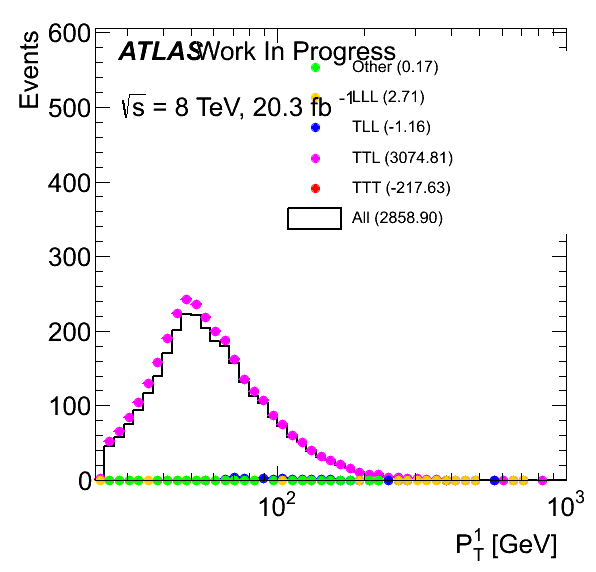
\includegraphics[width=.45\columnwidth]{figures/CompareMxMComponents/ChargeSameSign_PreselCustomRates_Mar19/png/LeadingLeptonPt.png}
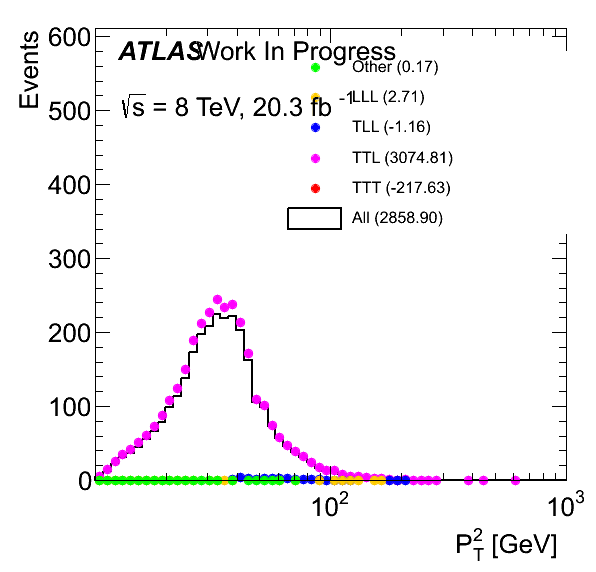
\includegraphics[width=.45\columnwidth]{figures/CompareMxMComponents/ChargeSameSign_PreselCustomRates_Mar19/png/SubleadingLeptonPt.png}
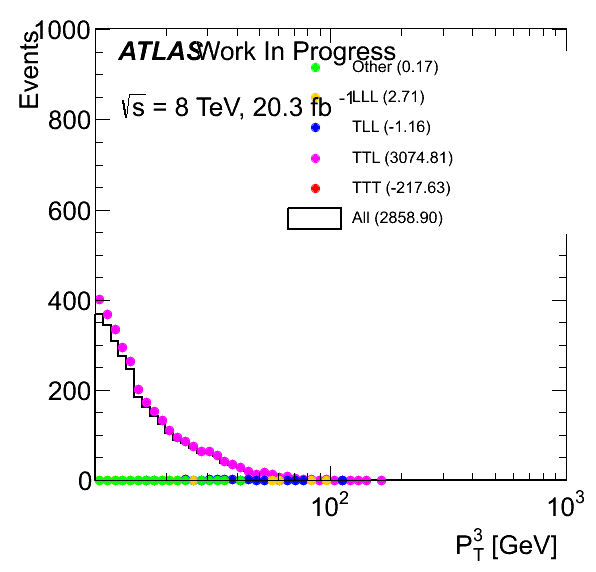
\includegraphics[width=.45\columnwidth]{figures/CompareMxMComponents/ChargeSameSign_PreselCustomRates_Mar19/png/MinimumLeptonPt.png}
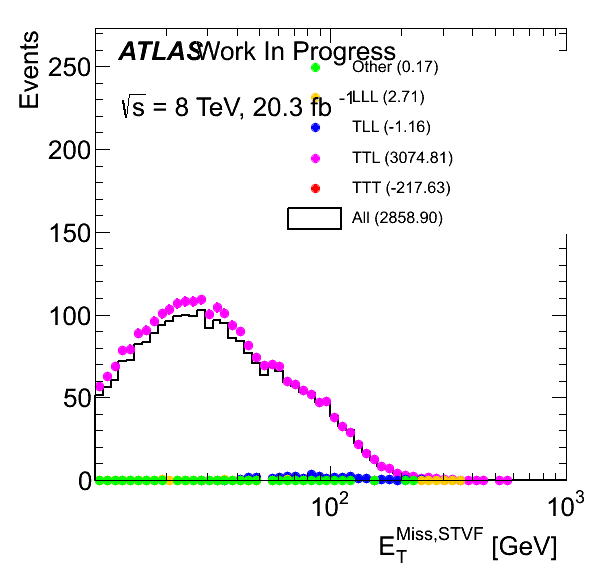
\includegraphics[width=.45\columnwidth]{figures/CompareMxMComponents/ChargeSameSign_PreselCustomRates_Mar19/png/MET_Et_STVF.png}
\caption{Fake background estimate at pre-selection broken
into tight and loose lepton configuration components for the 
leading (top left), sub-leading (top right), and minimum lepton \pt~(bottom left)
as well as the \met~(bottom right). The three lepton TTT (orange dots),
TTL (pink dots), TLL (blue dots), and LLL (yellow dots) components
are shown along with any other components (green dots) such as those
with four leptons initially.  The sum of all these components is also
shown (black line). (what if I showed the absolute value of these weights?)}
\label{fig:mxm_components}
\end{figure}


In the analysis, a specialized code is used to evaluate the 
Generalized Matrix Method
on all possible combinations of input and output leptons and checks
to see which leptons pass the final selection. 
It uses the on-the-fly
weighting method described above and uses a tensor
formulation that improves the computational efficiency of the method.
This is also used as described in \cite{Gillam:2014xua}.
Uncertainties are calculated by propagating through 
the uncertainties on the rates. 
Using the standard propagation of uncertainty, this relies
on the derivative of the expectation with respect to the rates.
Fortunately, this can be calculated in a straightforward way,
though it will not be described here.
Correlations between different bins are assumed to be negligible and 
are ignored.  However, since the method relies on calculating multiple
weights from the same event, there is a correlation in the uncertainty
if these weights end up falling in the same bin. To handle this 
correlation the uncertainty for these weights are added linearly 
as opposed to in quadrature when extracting the final uncertainty 
on the method. The effect of treating the correlation on the uncertainy is observed to
be mostly negligible.

\subsubsection{Rate Determination}
\label{sec:fake_and_real_rates}

The Generalized Matrix Method relies on being able to determine
the real and fake rates to be used as inputs to the method.
This is usually done by looking into control regions
which are designed to be enhanced in sources of real and fake leptons.
It is important to note that we can never know with certainty 
whether a lepton is real or fake. Instead we must be clever enough
to find leptons that we are confident are of the appropriate type.
One clever trick is to use a method called the tag-and-probe method
to better identify real or fake leptons in the control regions;
it will be described shortly.
Once we have obtained our two separate collections of leptons,
one we believe to be rich in real leptons and the other in fake leptons,
we can use these leptons to extract the real and fake rates, respectively.
The real rate, $\real^i$, in category (or bin) $i$,
is simply defined as the ratio of tight candidate real leptons
over the number of tight plus loose candidate real leptons:
\begin{equation}
\label{eq:real_rate}
\real^i = \frac{r_T^i}{r_T^i+r_L^i}
\end{equation}
where $r_T^i$ and $r_L^i$ are the number of tight and loose candidate
real leptons in category $i$, to be 
distinguished from the $n_T^i$ and $n_L^i$ which
are the number of candidate and loose real leptons in the signal regions
and whose origin is unknown.
Similarly, the fake rate, $\fake^i$, in category $i$, 
is defined as the ratio of tight candidate fake leptons over
the number of tight plus loose candidate fake leptons:
\begin{equation}
\label{eq:fake_rate}
\fake^i = \frac{f_T^i}{f_T^i+f_L^i}
\end{equation}
where $f_T^i$ and $f_L^i$ are the number of tight and loose candidate
fake leptons in category $i$.

The real and fake rates are not universally the same for all leptons, 
and in fact can vary strongly. Thus, the choice of categories, $i$, is
an important one. The rates are usually split by lepton
flavor and also in bins of at least one kinematic quantity.
The splitting of the categories by flavor is 
very important as the rates are 
typically very different for electrons and muons. 
This is in part because
the loose and tight selections are usually chosen to be different
by necessity.
The tight selections are the same as in \sec\ref{sec:object_selection}
for both electrons and muons.  The loose selections, however,
are similar to the tight selection except that
the isolation requirements are removed and the object quality 
classification is loosened for electrons.
Another reason for categories by lepton flavor
is that the control regions which are enhanced in real and fake sources
of leptons are typically different for electrons and muons.
Thus, we choose to evaluate the rates separately for both.


The rates also tend to vary as a function of the lepton kinematics.
Thus, we further divide the electron
and muon categories into sub-categories of mutually exclusive bins of
$\pt$. The number of bins and the bin edges are determined 
to best capture the shape while also maintaining adequate statistics
in each category. In practice it is usually not possible to subdivide
the \pt~by more than a few bins. For the same reason, while
the rates also surely vary according to other kinematic criteria, 
like $\eta$, it is usually not possible to subdivide in more than
one kinematic variable and still have good statistics.


The control regions are chosen so as to be dominated by a single 
physics process.  For determining the real rates, the 
control region is chosen to be enhanced in $Z\rightarrow ll$
while the control region for determining the fake rates is
chosen to be enhanced in 
$W\rightarrow l\nu$ plus jets.
The reason for this choice is to allow for the application of the
tag-and-probe method, which uses one well defined lepton, the
``tag'', to identify the process, and another lepton, the ``probe'',
as the lepton under study. Both of these control regions
have at least one lepton object. 

\begin{figure}[ht!]
\centering
\subfigure{
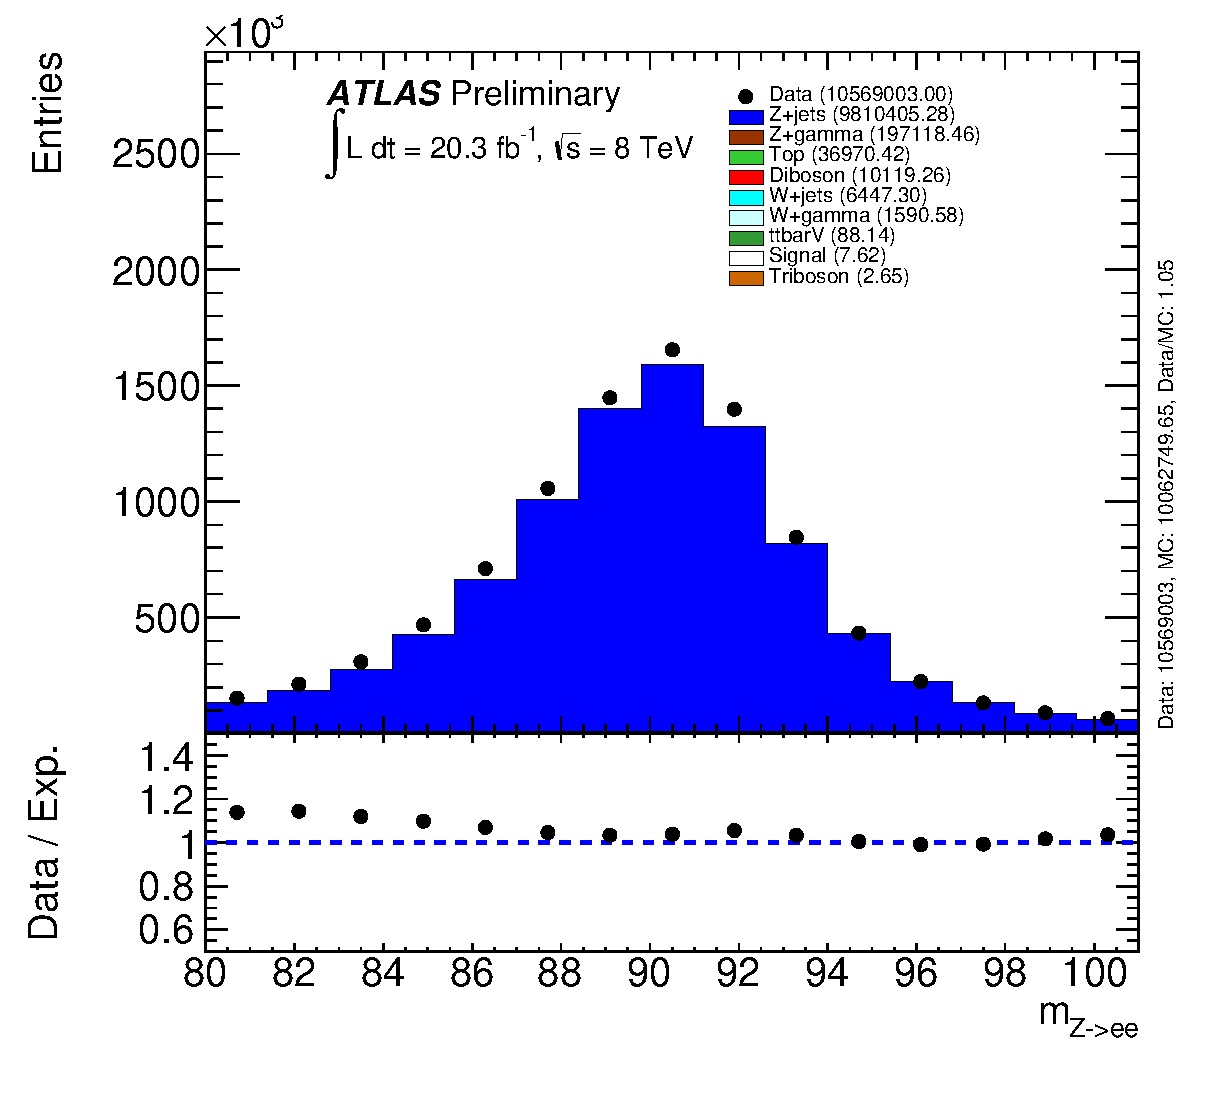
\includegraphics[width=0.4\columnwidth]{figures/fakes_bkg/CRs/hPtElectronZBosonloosecut_total_new.eps}
}
\centering
\subfigure{
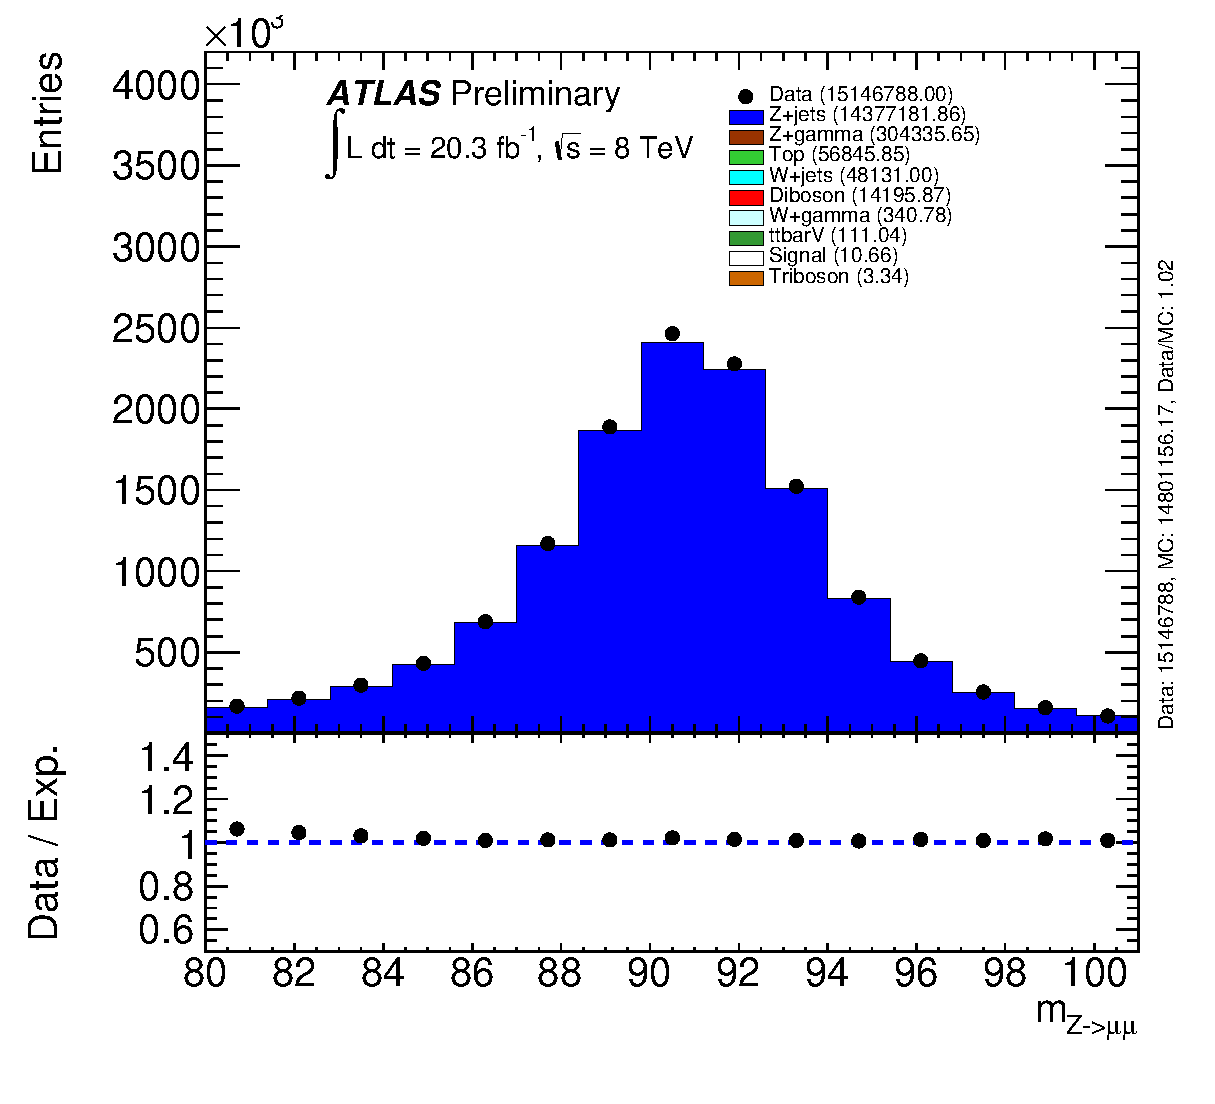
\includegraphics[width=0.4\columnwidth]{figures/fakes_bkg/CRs/hPtMuonZBosonloosecut_total_new.eps}
}
\vspace{-10mm}\caption{Invariant mass distribution of two opposite charge and same flavor di-lepton invariant mass electrons (left) and muons (right). Update figures!!}
\label{fig:realEff_CRs}
\end{figure}

\begin{figure}[ht!]
\centering
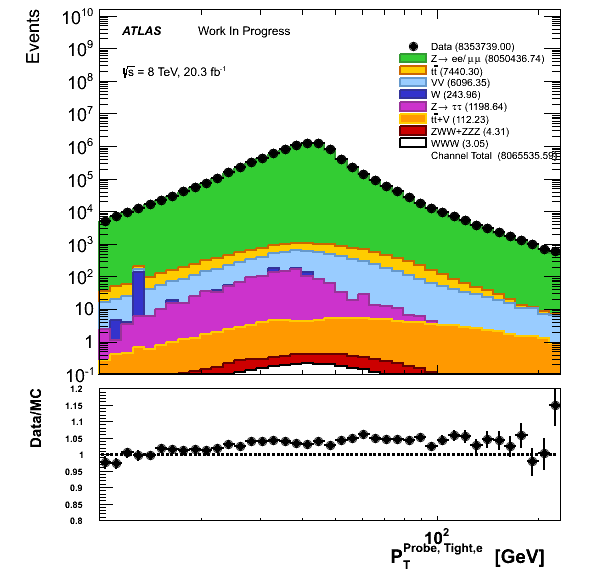
\includegraphics[width=0.4\columnwidth]{figures/fakes_bkg/CRs/RealTP/ProbeTightElectronPt_histratio.png}
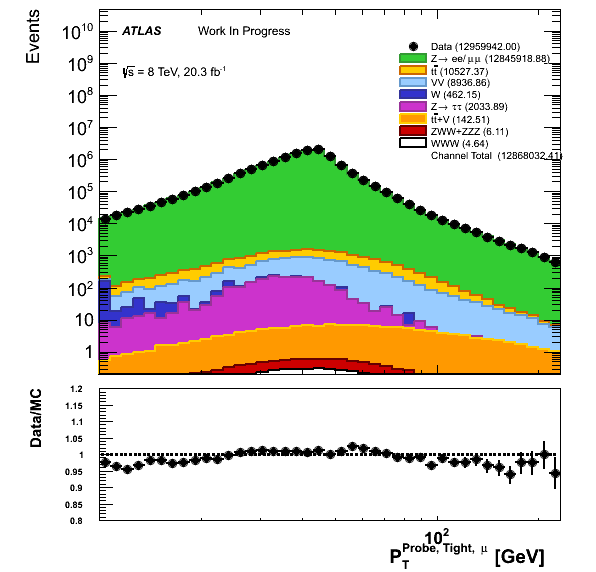
\includegraphics[width=0.4\columnwidth]{figures/fakes_bkg/CRs/RealTP/ProbeTightMuonPt_histratio.png}
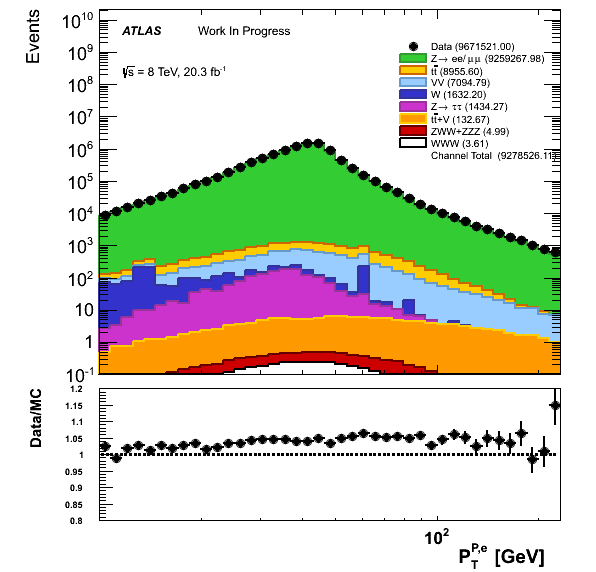
\includegraphics[width=0.4\columnwidth]{figures/fakes_bkg/CRs/RealTP/ProbeElectronPt_histratio.png}
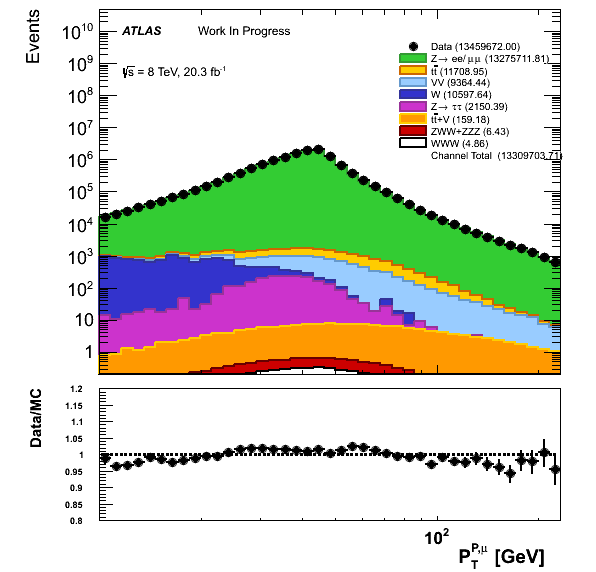
\includegraphics[width=0.4\columnwidth]{figures/fakes_bkg/CRs/RealTP/ProbeMuonPt_histratio.png}
\caption{Probe lepton \pt\ distributions in SFOS tag and probe control regions used to derive real rates.  Electron (left) and muon (right) are shown
when the probe lepton is either tight (top) or no additional selection (besides the pre-selection) is required (bottom)}
\label{fig:realEff_CRsPt}
\end{figure}

In the control regions enhanced
in $Z\rightarrow ll$, if one well-reconstructed 
tag lepton passing the tight selection is found then the presence
of an additional lepton will almost certainly be the other real
lepton from the $Z$ decay. Thus, this second ``probe''
lepton, which can pass either the loose or tight selection
requirement is our candidate real lepton.
Note that if the probe lepton also passes the tight selection
then it could also be used as a tag. In fact, ignoring
this possibility can introduce a bias. Thus, we consider both 
leptons as either tag or probe candidates.
Only events where 
the tag lepton passes the same single lepton triggers and trigger
matching requirements as in \sec\ref{sec:event_selection} are used. 
We also require the presence of a 
probe lepton that forms an SFOS pair with the
tag whose di-lepton mass is within 10~\GeV of the \z-mass.
Two control regions are formed: one from $e^{+}e^{-}$ tag-probe
pairs for determining the electron real rates and another
from $\mu^{+}\mu^{-}$ tag-probe pairs for determining the muon
real rates. The \z-peak in the 
di-lepton invariant mass distribution for the two control regions
are shown in \fig\ref{fig:realEff_CRs} comparing the data
to the model.
Since the rates are also determined as a function of the lepton
\pt, the lepton \pt~distributions are shown in 
\fig\ref{fig:realEff_CRsPt}
for the data as well as the expectation.
They are show separately for electrons
and muons and based on whether the probe leptons
pass just the tight selection 
(the top row of \fig\ref{fig:realEff_CRsPt})
or both the loose and tight selections
(the bottom row of \fig\ref{fig:realEff_CRsPt}).
The data clearly agrees well with the expectation, which is dominated
by the $Z\rightarrow ll$ process, as expected. The ratio of the 
candidate real leptons passing just the tight selection 
over those passing the loose and tight selections 
determines the real rate according to \eqn\eqref{eq:real_rate}.

The real rates are shown separately for electrons and muons 
in \fig\ref{fig:realEff} after adjusting to a coarser binning
to improve the statistics. 
It is interesting to note that the real rates
are uniformly lower for electrons than for muons, but both follow
the same trend of increasing as a function of the lepton \pt, 
and are relatively high even for the lowest value of 81\%.
The difference between the rates calculated 
either the data or the MC exclusively 
is taken as a systematic uncertainty on the nominal estimate
from the data. 
The rates and the systematic uncertainties
are summarized for electrons
in \tab\ref{tab:realEff_El} and for muons in \tab\ref{tab:realEff_Mu}.




\begin{figure}[ht!]
\centering
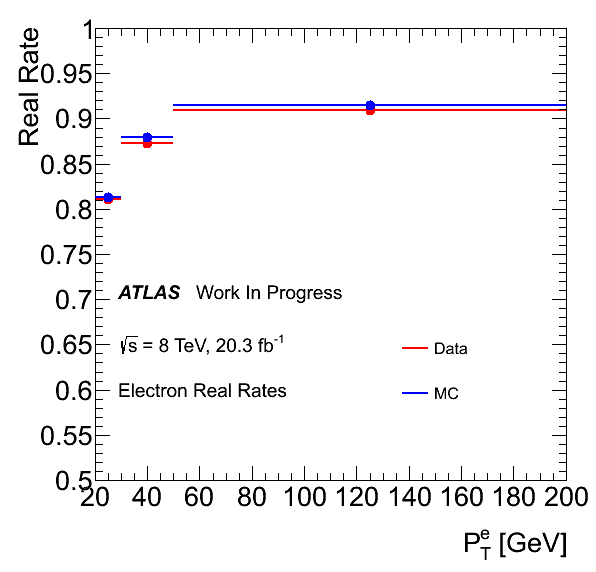
\includegraphics[width=0.45\columnwidth]{figures/fakes_bkg/Efficiencies/ElectronRealRates.png}
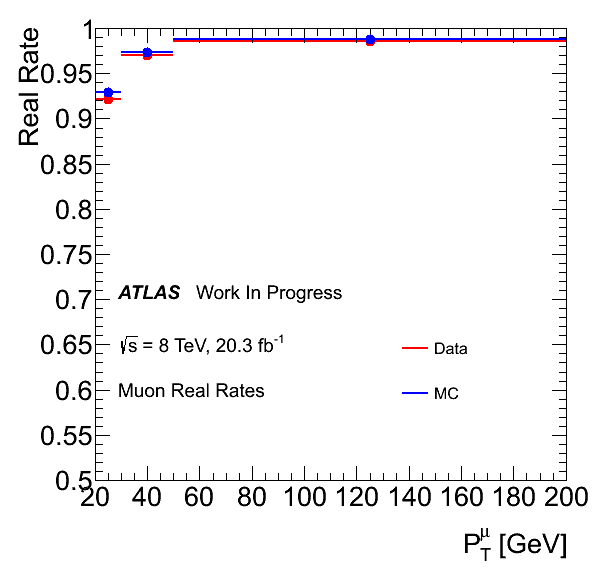
\includegraphics[width=0.45\columnwidth]{figures/fakes_bkg/Efficiencies/MuonRealRates.png}
\caption{Real lepton efficiency as a function of \pt\ and measured in data (red) and MC (blue) for electrons (left) and muons (right).}
\label{fig:realEff}
\end{figure}


%\tabcolsep=0.11cm
\begin{table}[ht!]
\centering
\begin{tabular}{|l||c|c||c|c||c|}
\hline
&\multicolumn{2}{c||}{Data}&\multicolumn{2}{c||}{MC}&\multicolumn{1}{c|}{}\\ & $\varepsilon_r$ & $\sigma_{stat}$ & $\varepsilon_r$ & $\sigma_{stat}$ & $\sigma_{sys}$\\ 
\hline\hline
%$p_{T}\in[10,15]$ GeV &  $0.6285$ &  $0.0034$ &  $0.6420$ &  $0.0036$ &  $0.0135$\\ 
%$p_{T}\in[15,20]$ GeV &  $0.6960$ &  $0.0024$ &  $0.7056$ &  $0.0025$ &  $0.0096$\\ 
$p_{T}\in[20,30]$ GeV &  $0.8105$ &  $0.0011$ &  $0.8134$ &  $0.0013$ &  $0.0028$\\ 
$p_{T}\in[30,50]$ GeV &  $0.8732$ &  $0.0005$ &  $0.8794$ &  $0.0006$ &  $0.0062$\\ 
$p_{T} > 50$ GeV &  $0.9097$ &  $0.0012$ &  $0.9150$ &  $0.0012$ &  $0.0053$\\ 
\hline
\end{tabular}

\caption{Measured real efficiencies for electrons including statistical and systematic absolute uncertainties. 
Systematic is calculated by taking the difference
between the efficiencies measured in data and MC.  The efficiency measured in data is used as the nominal central value.
} 
\label{tab:realEff_El}
\end{table} 

%\tabcolsep=0.11cm
\begin{table}[ht!]
\centering
\begin{tabular}{|l||c|c||c|c||c|}
\hline
&\multicolumn{2}{c||}{Data}&\multicolumn{2}{c||}{MC}&\multicolumn{1}{c|}{}\\ & $\varepsilon$ & $\sigma_{stat}$ & $\varepsilon$ & $\sigma_{stat}$ & $\sigma_{sys}$\\ 
\hline\hline
%$p_{T}\in[10,15]$ GeV &  $0.8684$ &  $0.0033$ &  $0.8763$ &  $0.0036$ &  $0.0079$\\ 
%$p_{T}\in[15,20]$ GeV &  $0.8906$ &  $0.0024$ &  $0.8956$ &  $0.0025$ &  $0.0050$\\ 
$p_{T}\in[20,30]$ GeV &  $0.9217$ &  $0.0010$ &  $0.9291$ &  $0.0012$ &  $0.0074$\\ 
$p_{T}\in[30,50]$ GeV &  $0.9700$ &  $0.0004$ &  $0.9737$ &  $0.0006$ &  $0.0038$\\ 
$p_{T} > 50$ GeV &  $0.9862$ &  $0.0011$ &  $0.9878$ &  $0.0011$ &  $0.0017$\\ 
\hline
\end{tabular}

\caption{Measured real efficiencies for muons including statistical and systematic absolute uncertainties.
Systematic is calculated by taking the difference
between the efficiencies measured in data and MC.  The efficiency measured in data is used as the nominal central value.
} 
\label{tab:realEff_Mu}
\end{table} 


On the other hand, in the 
$W\rightarrow l\nu + \textrm{Jets}$ control region there
is only one real lepton being produced by the process.
If a well reconstructed tag lepton passing the tight selection
is found in this control 
region it is most likely coming from the $W$ decay.
In this case, if we measure a second ``probe'' lepton it is most likely
a jet faking a lepton. Thus, we have found a candidate fake lepton.
The control regions are formed by requiring the presence
of one tag lepton passing the tight selection
plus trigger requirements
of \sec\ref{sec:event_selection} with a $\pt>40\GeV$ and 
a probe lepton passing either the loose or tight selection.
The leptons are required to have the same sign, since
on average a fake lepton will have equal probably of
a positive or negative charge, while background processes
like $WW$,$\ttbar$, and $Z$ production produce opposite-sign lepton
pairs.  Only muons are used as tag leptons. 
The reason for this is that the chance of an electron passing tight selection
to be a jet fake is higher than that for muons. It is also 
possible for electrons to come from photon conversion  (PC)
while for muons this is very unlikely. Thus, using only muons as tag
leptons further reduces contamination from backgrounds in this control
region. The control region is then split based on whether the probe
lepton is an electron or a muon in order to determine the electron
and muon fake rates separately.
Events with additional leptons are thrown away.
To suppress contamination from multi-jet background processes
to the $W\rightarrow l\nu + \textrm{Jets}$ process, like QCD,
a cut of $\met>10\GeV$ is also applied.

The fake rate that is determined depends upon the source of fake leptons.
One way to assess this sensitivity is to consider the number of
\bee-jets present in the event. We consider two different
cases regarding the \bee-jet multiplicity: inclusive and exclusive.
The inclusive case makes no requirement on the number of \bee-jets
while the exclusive case asks that at least one \bee-jet is present.
These two different scenarios are ultimately compared in order to assess
a final systematic on the fake rate. The exclusive case
is used as the nominal estimate.

\begin{figure}[ht]
\centering
\subfigure{
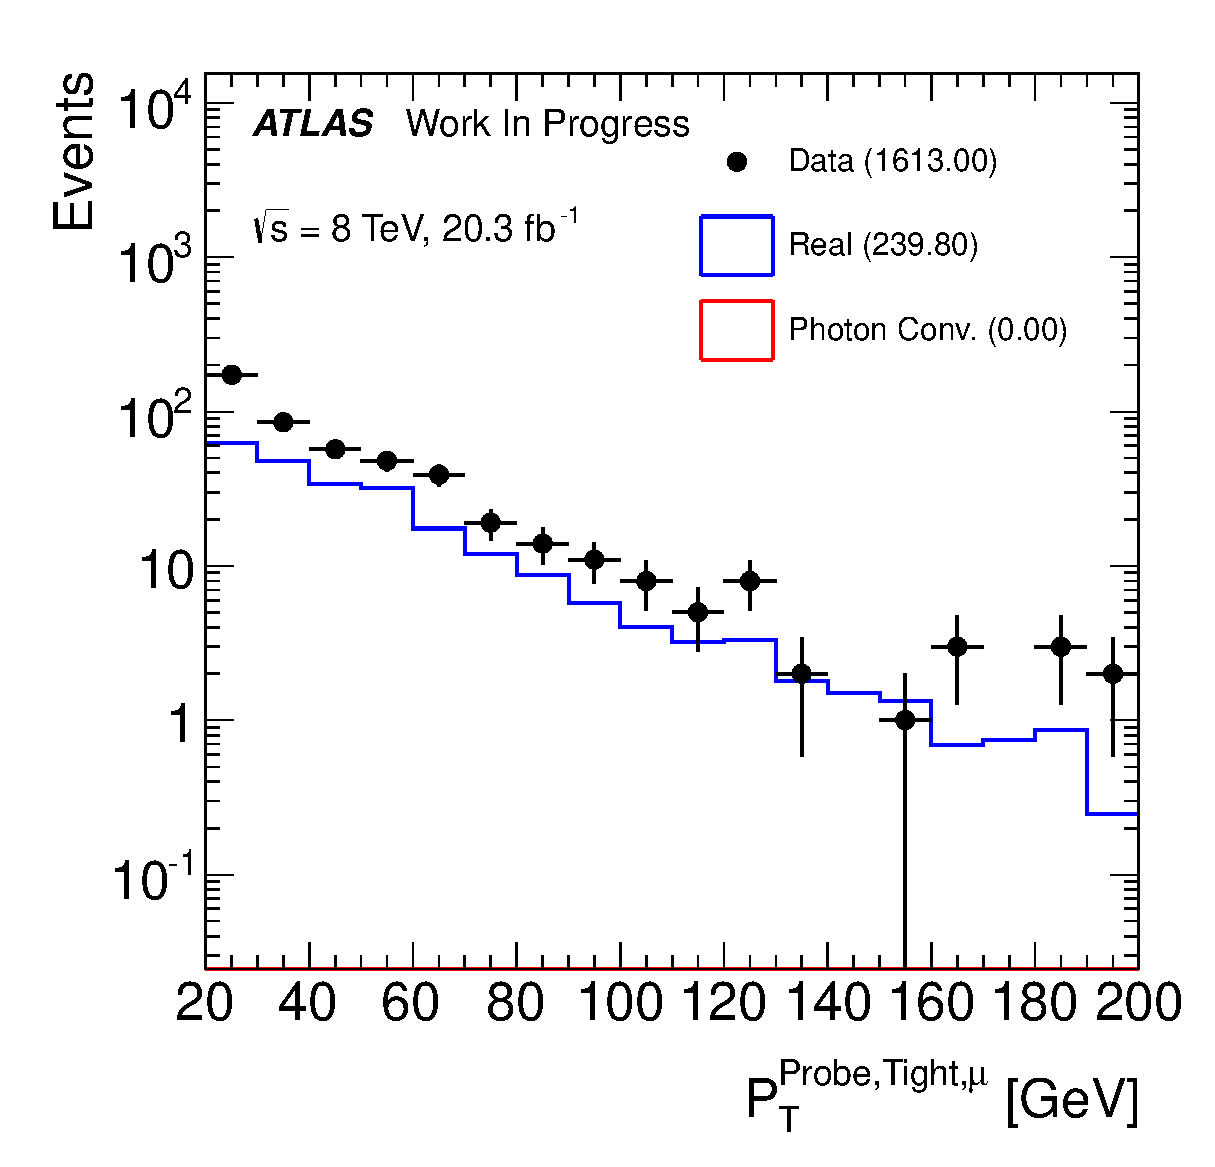
\includegraphics[width=0.45\columnwidth]{figures/fakes_bkg/CRs/SameSignMuonMuon/NoStack/ProbeTightMuonPt.eps}
}
%\centering
%\subfigure{
%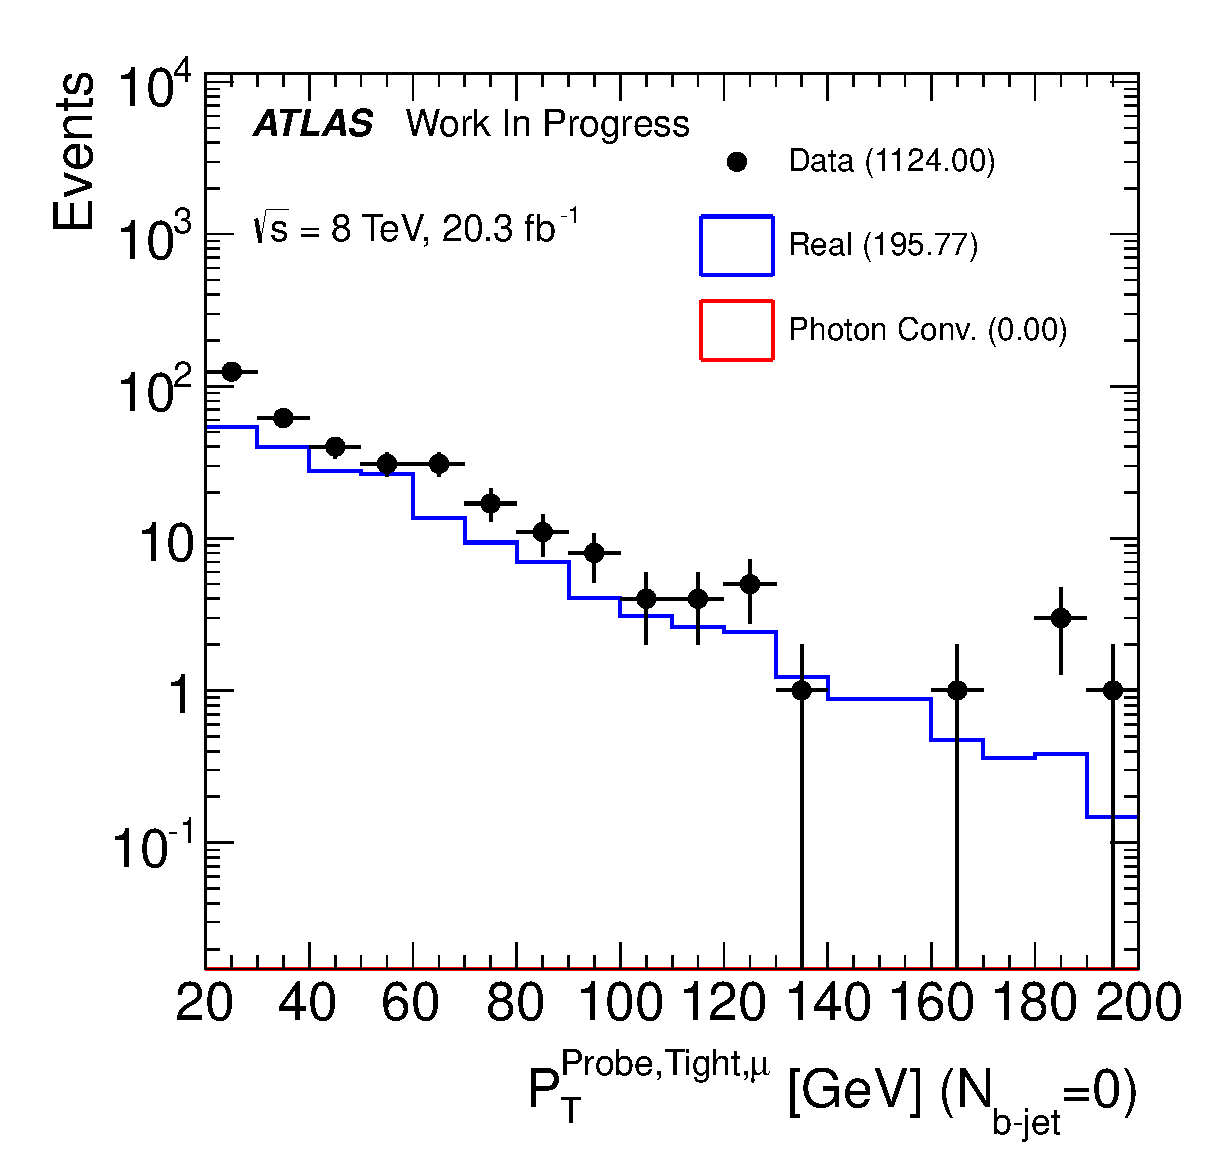
\includegraphics[width=0.3\columnwidth]{figures/fakes_bkg/CRs/SameSignMuonMuon/NoStack/ProbeTightMuonPtBJetEq0.eps}
%}
\centering
\subfigure{
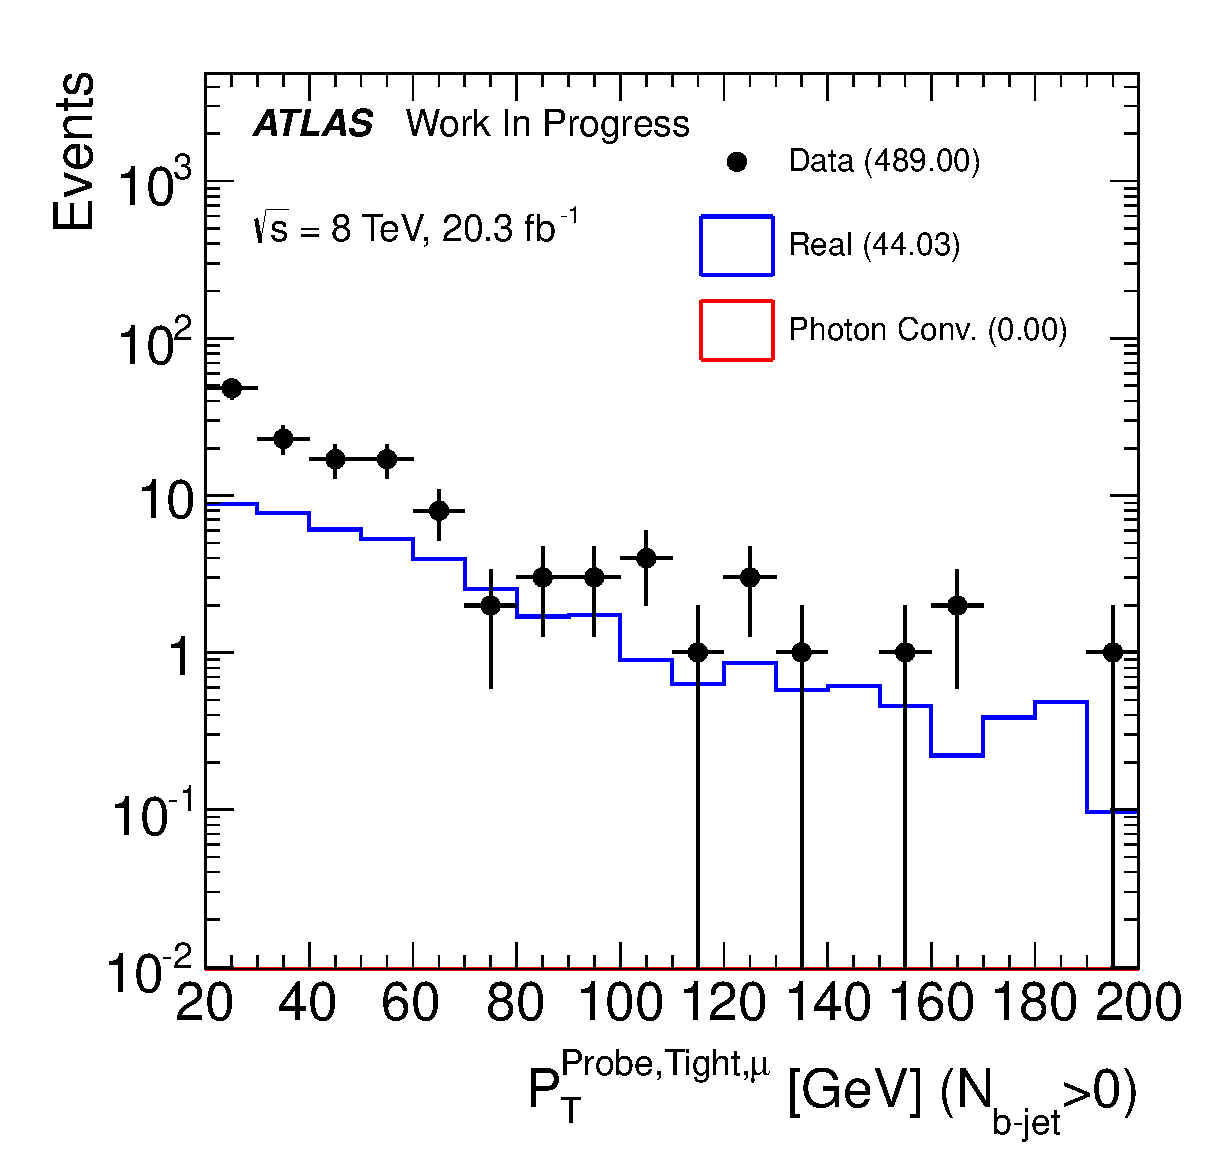
\includegraphics[width=0.45\columnwidth]{figures/fakes_bkg/CRs/SameSignMuonMuon/NoStack/ProbeTightMuonPtBJetGt0.eps}
}
%\vspace{-1mm}
\centering
\subfigure{
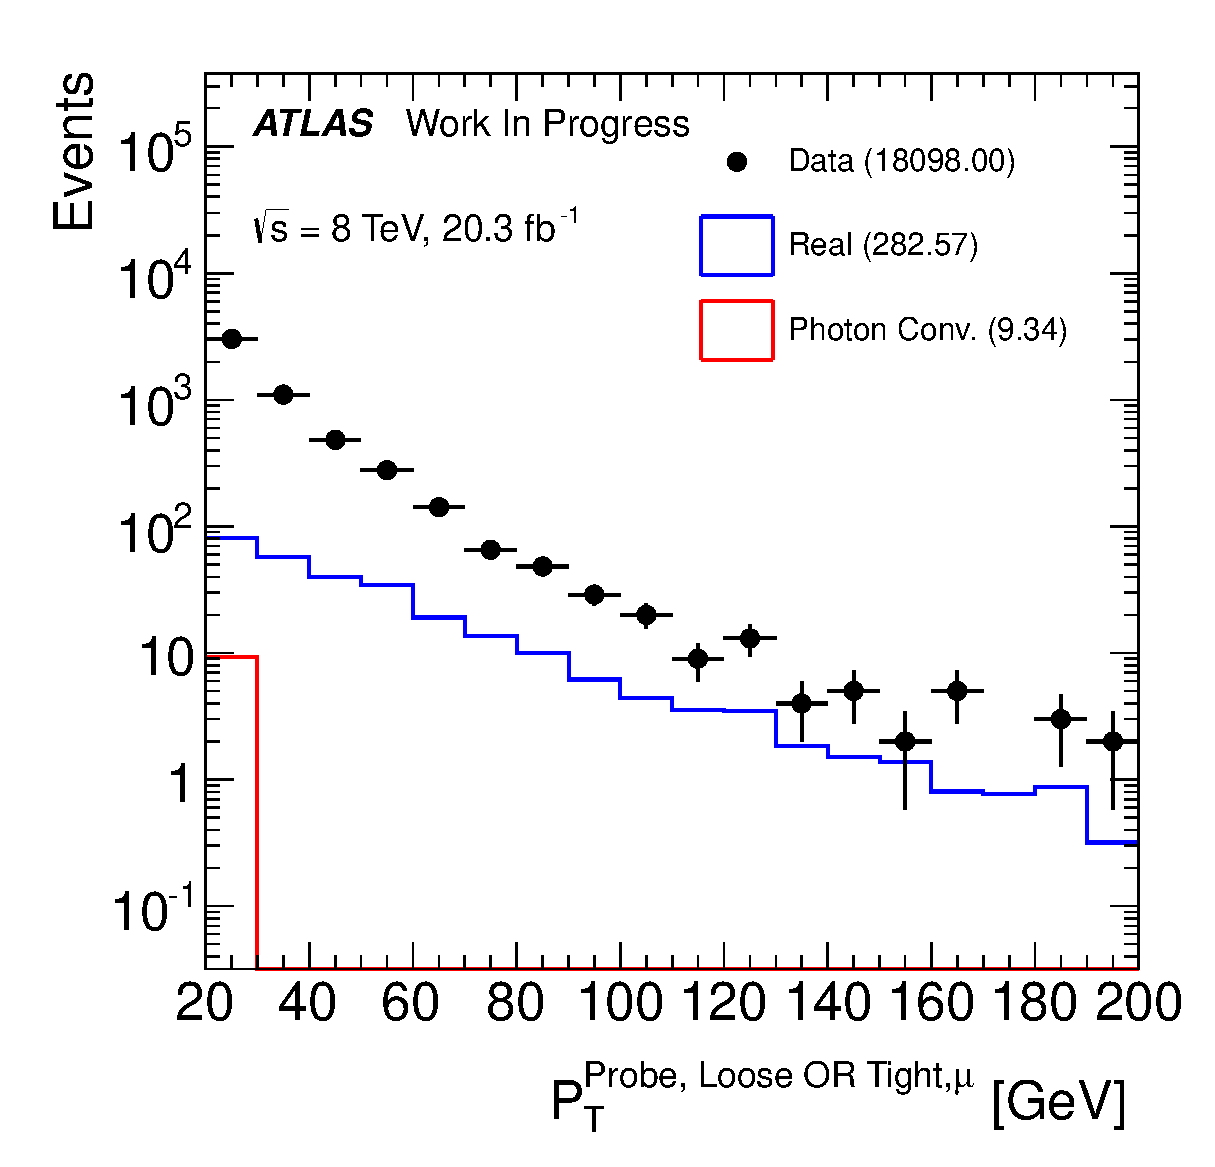
\includegraphics[width=0.45\columnwidth]{figures/fakes_bkg/CRs/SameSignMuonMuon/NoStack/ProbeLooseORTightMuonPt.eps}
}
%\centering
%\subfigure{
%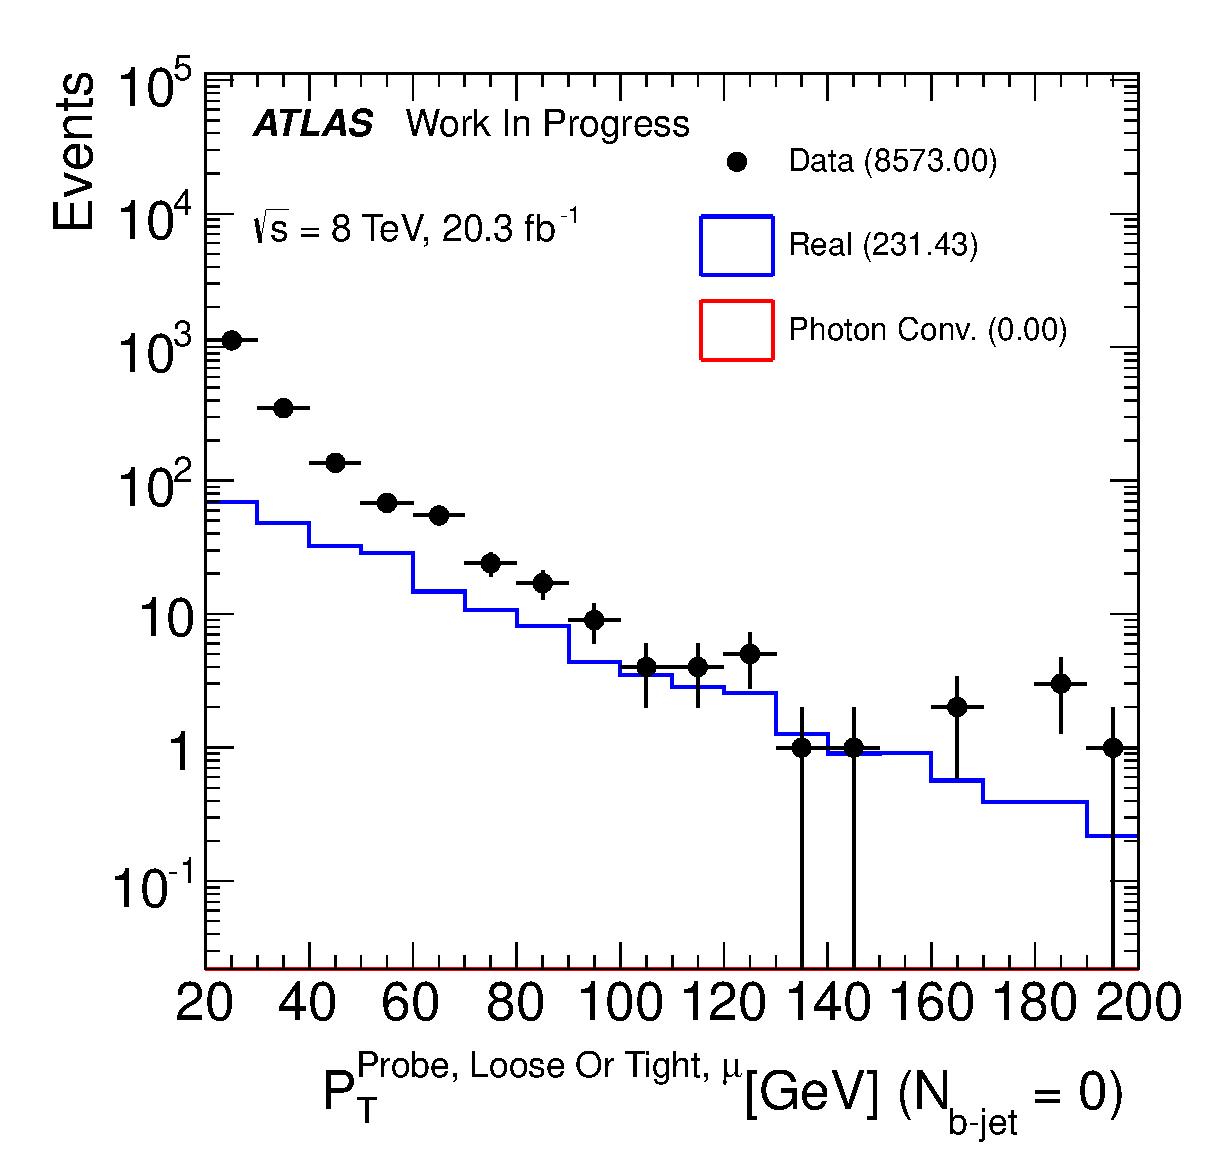
\includegraphics[width=0.45\columnwidth]{figures/fakes_bkg/CRs/SameSignMuonMuon/NoStack/ProbeLooseORTightMuonPtBJetEq0.eps}
%}
\centering
\subfigure{
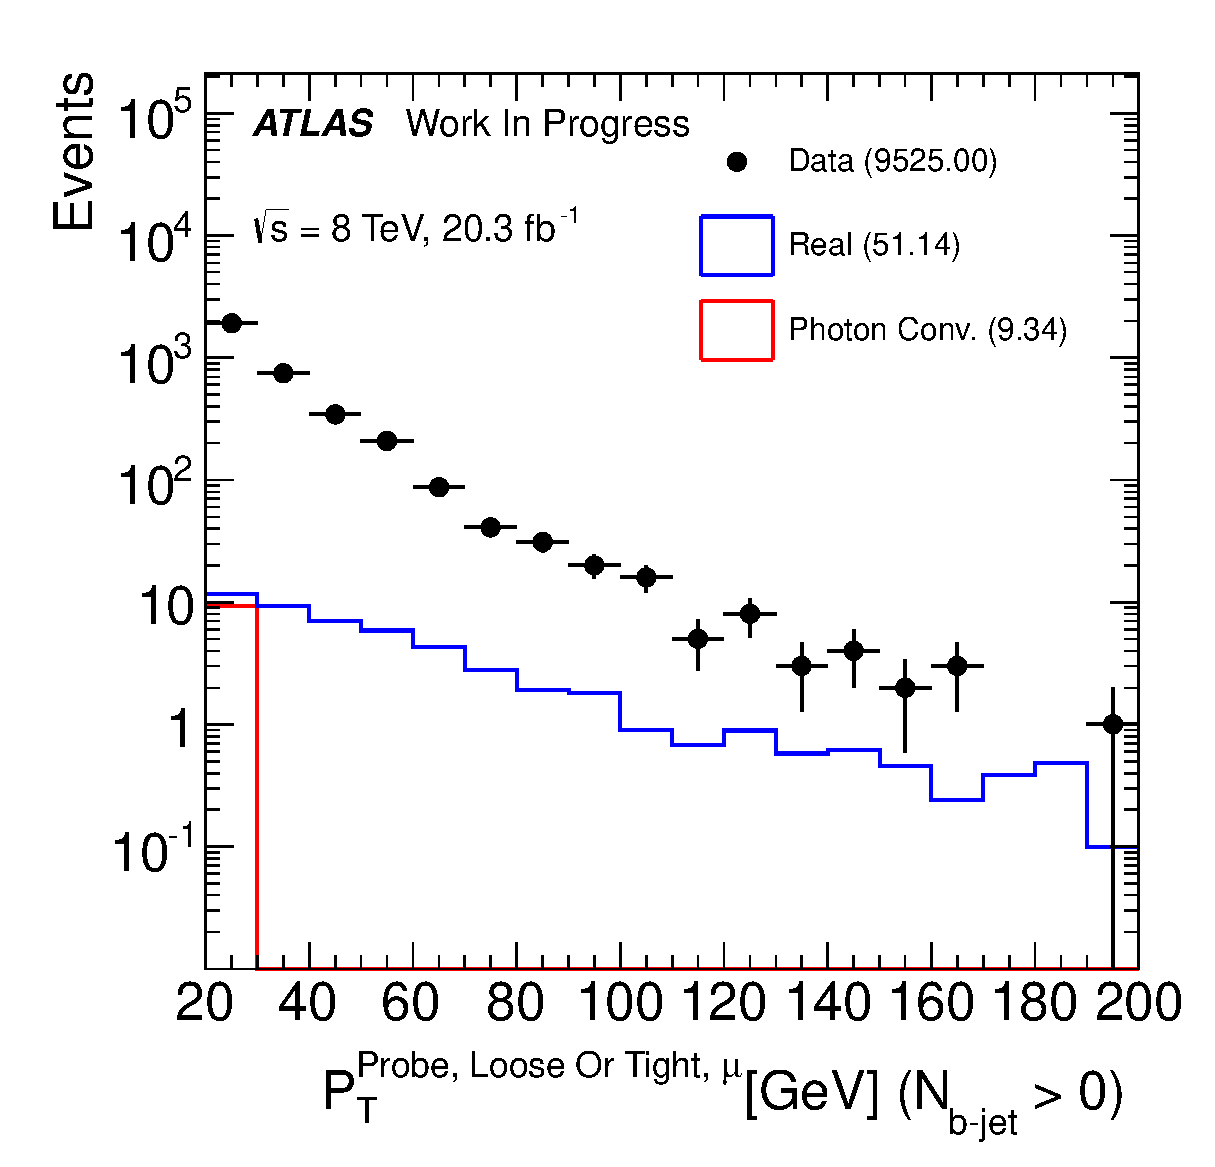
\includegraphics[width=0.45\columnwidth]{figures/fakes_bkg/CRs/SameSignMuonMuon/NoStack/ProbeLooseORTightMuonPtBJetGt0.eps}
}
%\vspace{-10mm}
\caption{Transverse momentum distributions \pt\ of tight probe 
muons (top) and loose OR tight probe muons (bottom) passing signal 
selection criteria in the control Same-Sign $\mu-\mu$ control region 
without any additional requirement on $b$-jets in the event (left) and 
at least one $b$-jet (right). 
The amount observed in data (black points) corresponds 
to $N_T^{\textrm{Data},i}+N_L^{\textrm{Data},i}$ (bottom) and $N_T^{\textrm{Data},i}$ (top) following the notation
in \eqn\ref{eq:fake_num_breakdown}.
Meanwhile, the contribution determined in MC to come from 
real leptons (blue line) and from photon conversion (red line) are shown 
separately; they are not stacked. The real lepton contribution corresponds to 
$N_T^{\textrm{Real},i}+N_L^{\textrm{Real},i}$ (bottom) and $N_T^{\textrm{Real},i}$ 
(top) and the photon conversion 
contribution 
corresponds to $N_T^{\textrm{PC},i}+N_L^{\textrm{PC},i}$ (bottom) 
and $N_T^{\textrm{PC},i}$ (top) again using the notation 
in Eq.~\ref{eq:fake_rate}. 
The photon conversion is 
observed to be negligible for muons.  }
\label{fig:fakeEff_CRs_muon}
\end{figure}

\begin{figure}[ht]
\centering
\subfigure{
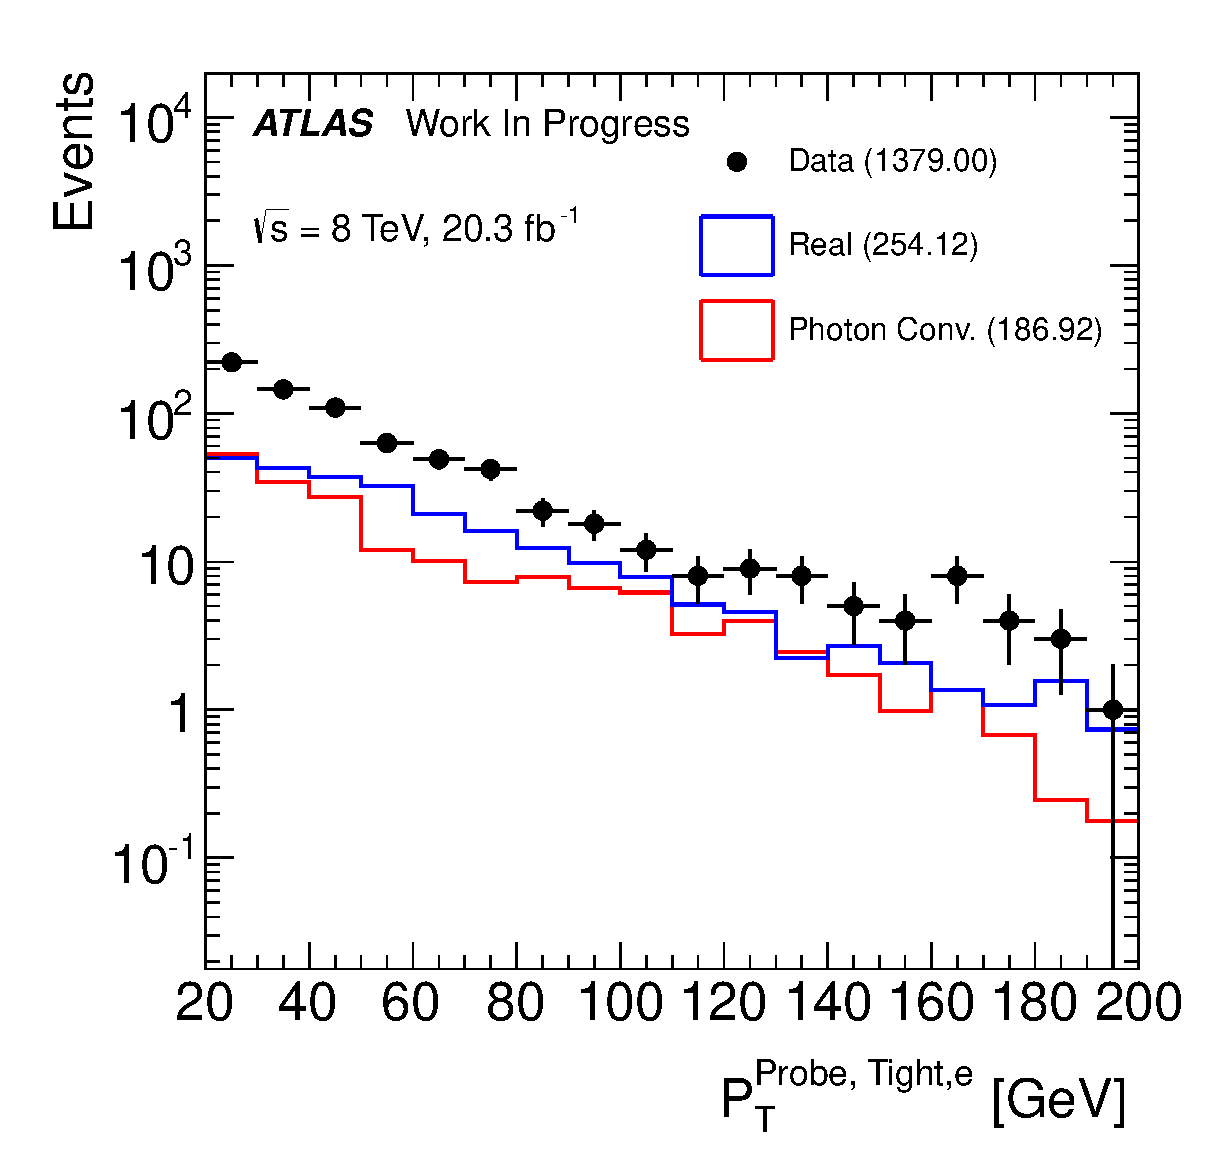
\includegraphics[width=0.45\columnwidth]{figures/fakes_bkg/CRs/SameSignElectronMuon/NoStack/ProbeTightElectronPt.eps}
}
%\centering
%\subfigure{
%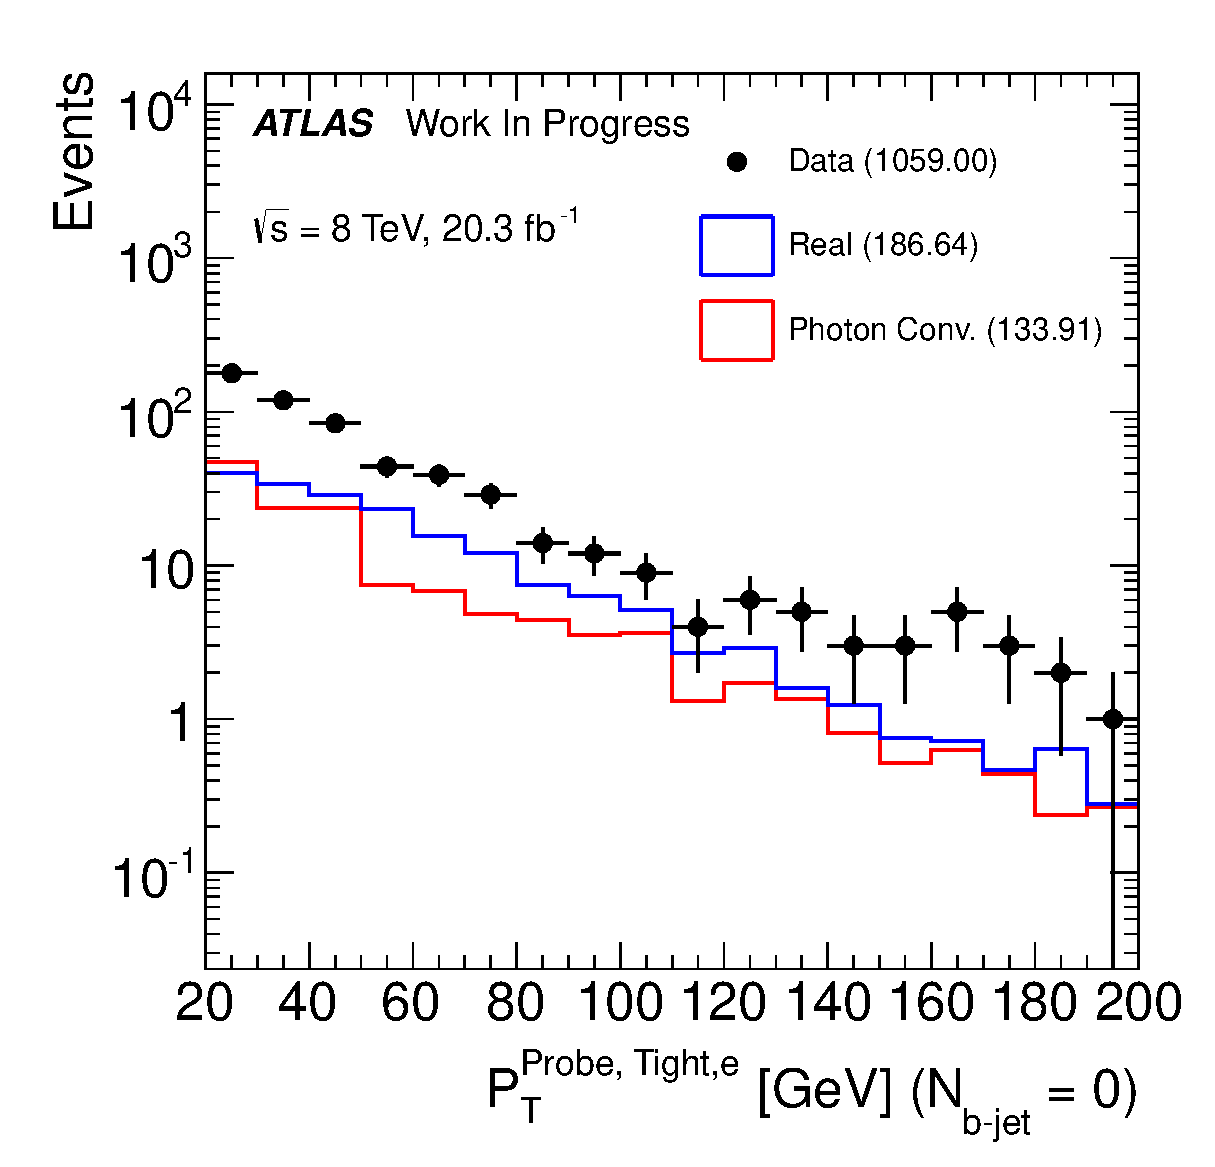
\includegraphics[width=0.3\columnwidth]{figures/fakes_bkg/CRs/SameSignElectronMuon/NoStack/ProbeTightElectronPtBJetEq0.eps}
%}
\centering
\subfigure{
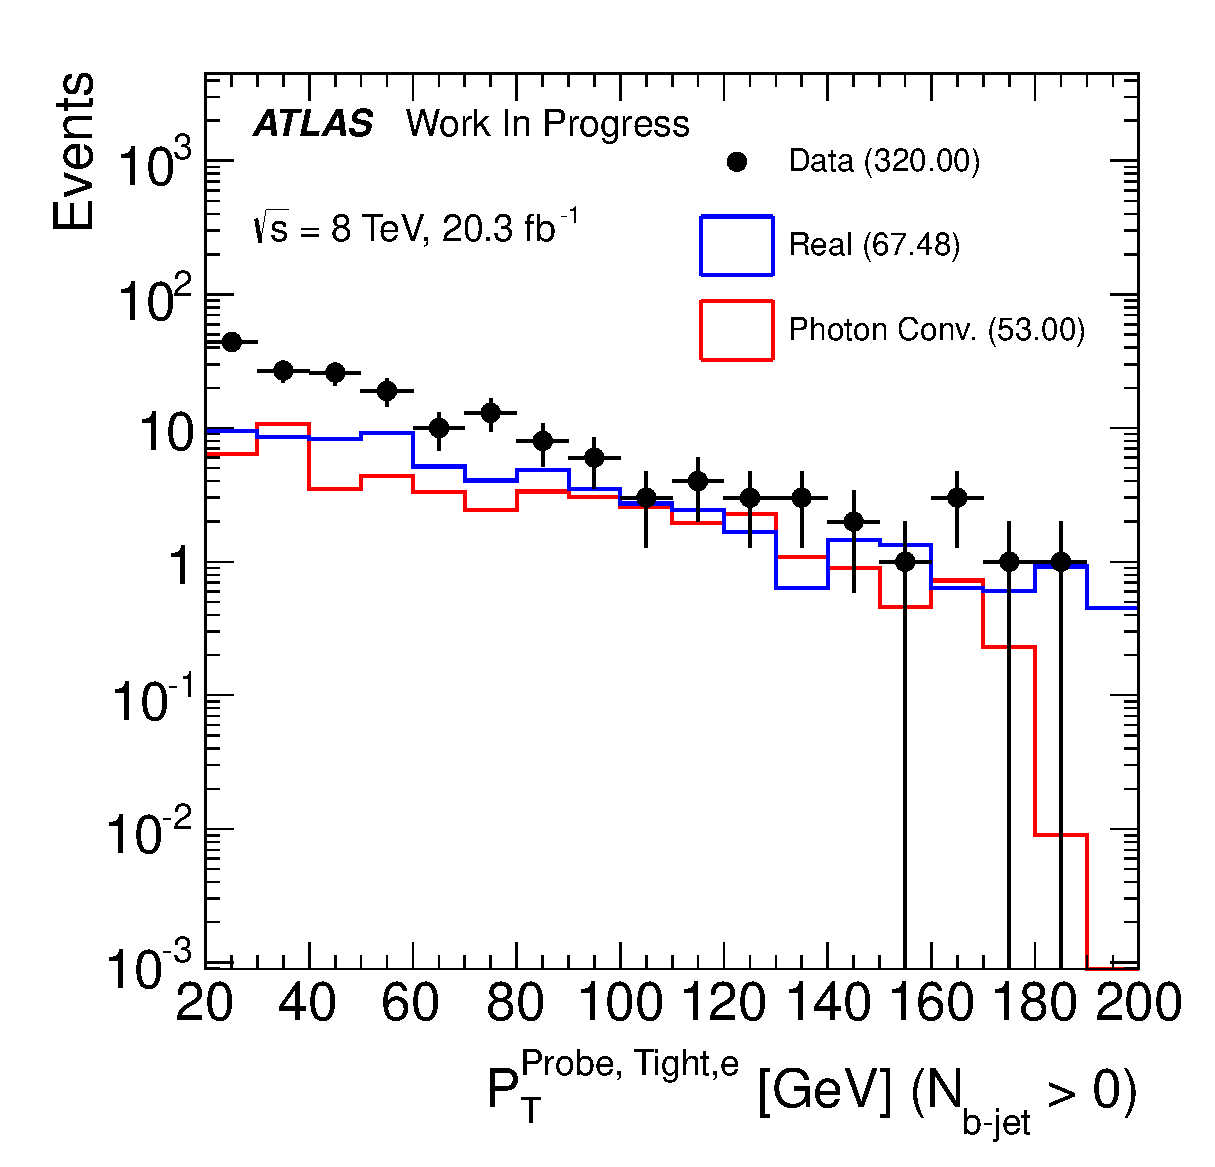
\includegraphics[width=0.45\columnwidth]{figures/fakes_bkg/CRs/SameSignElectronMuon/NoStack/ProbeTightElectronPtBJetGt0.eps}
}
\centering
\subfigure{
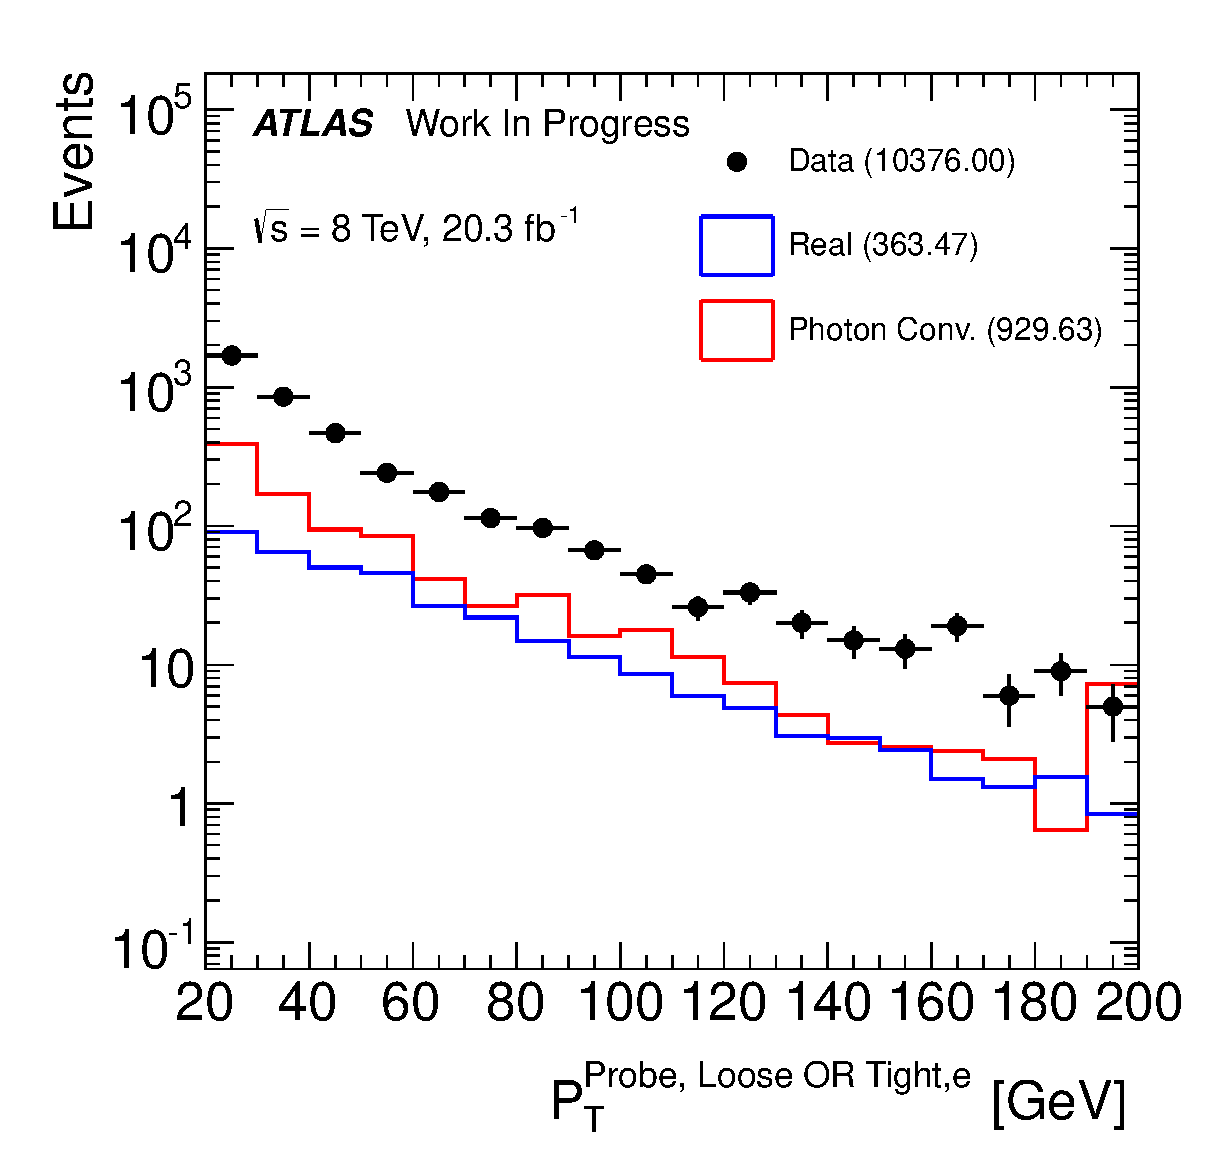
\includegraphics[width=0.45\columnwidth]{figures/fakes_bkg/CRs/SameSignElectronMuon/NoStack/ProbeLooseORTightElectronPt.eps}
}
%\centering
%\subfigure{
%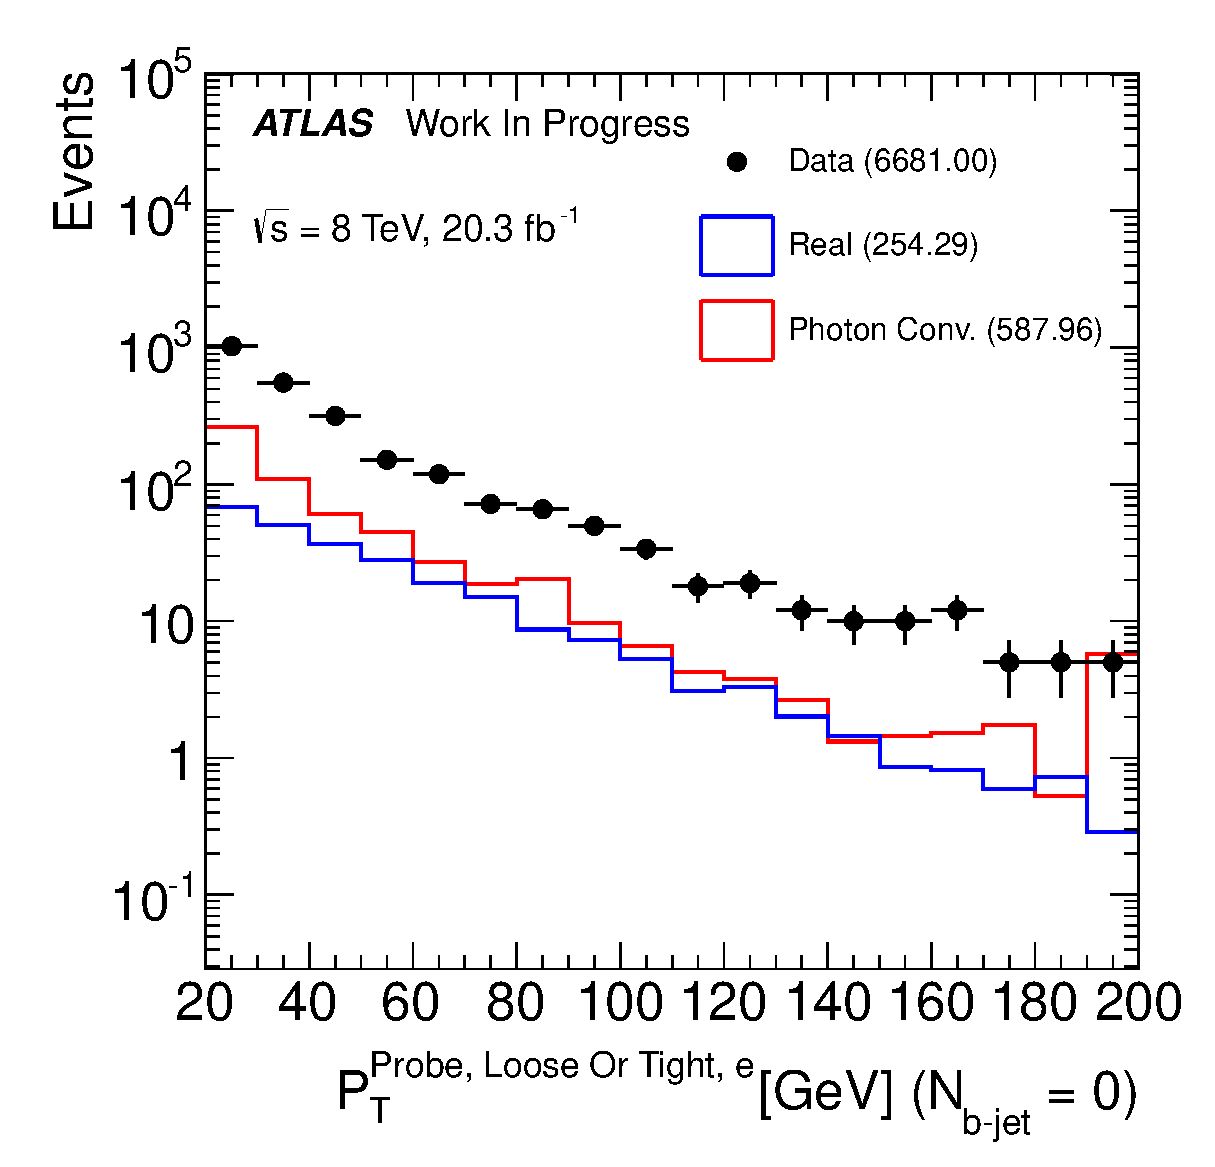
\includegraphics[width=0.3\columnwidth]{figures/fakes_bkg/CRs/SameSignElectronMuon/NoStack/ProbeLooseORTightElectronPtBJetEq0.eps}
%}
\centering
\subfigure{
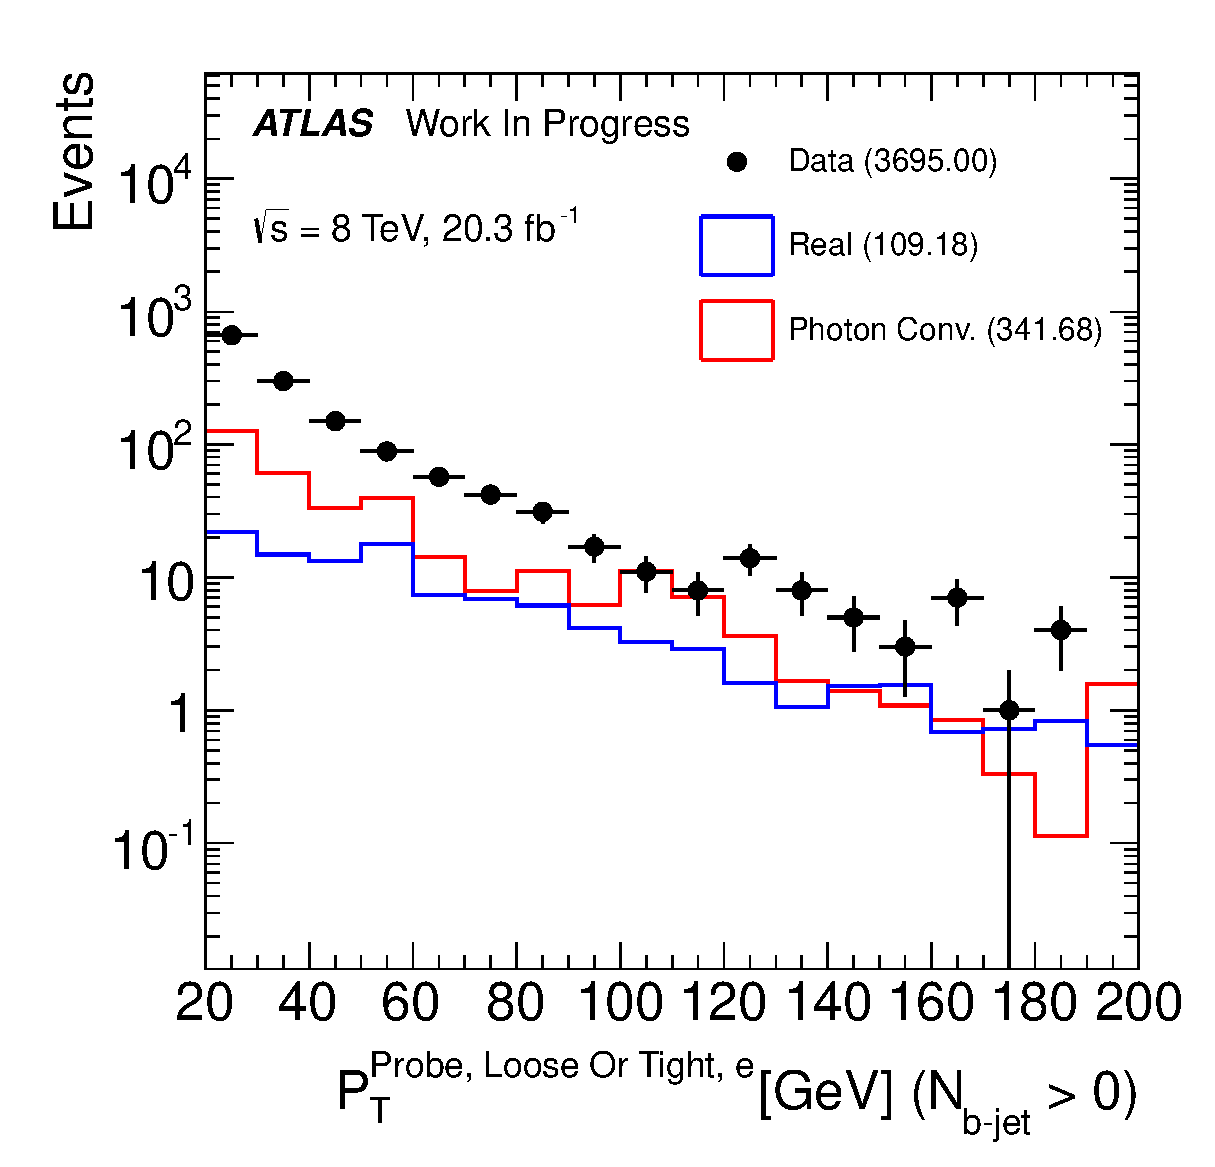
\includegraphics[width=0.45\columnwidth]{figures/fakes_bkg/CRs/SameSignElectronMuon/NoStack/ProbeLooseORTightElectronPtBJetGt0.eps}
}
%\vspace{-1mm}
%\vspace{-10mm}
\caption{Transverse momentum distributions \pt\ of tight probe 
electrons (top) and loose OR tight probe muons (bottom) passing signal 
selection criteria in the control Same-Sign $e-\mu$ control region 
without any additional requirement on $b$-jets in the event (left) and 
at least one $b$-jet (right). 
The amount observed in data (black points) corresponds 
to $N_T^{\textrm{Data},i}+N_L^{\textrm{Data},i}$ (bottom) and $N_T^{\textrm{Data},i}$ (top) following the notation
in \eqn\ref{eq:fake_num_breakdown}.
Meanwhile, the contribution determined in MC to come from 
real leptons (blue line) and from photon conversion (red line) are shown 
separately; they are not stacked. The real lepton contribution corresponds to 
$N_T^{\textrm{Real},i}+N_L^{\textrm{Real},i}$ (bottom) and $N_T^{\textrm{Real},i}$ 
(top) and the photon conversion 
contribution 
corresponds to $N_T^{\textrm{PC},i}+N_L^{\textrm{PC},i}$ (bottom) 
and $N_T^{\textrm{PC},i}$ (top) again using the notation 
in Eq.~\ref{eq:fake_rate}. }


\label{fig:fakeEff_CRs_electron}
\end{figure}

The processes contributing to the fake rate are known
to not be well modeled by MC, as discussed earlier in \sec\ref{sec:bg_fake}.
This is the primary reason for attempting to estimate the fake
lepton contribution from data in the first place. Thus,
we do not seek to describe the data using MC.
However, this control region is also not as pure with sources
of fake leptons as the real lepton control region is for real leptons,
because the neutrino in the $W\rightarrow l\nu$ control region
cannot be identified directly.
In particular, there is a significant contamination from processes
with real leptons, like $WW$, $\ttbar$, and $Z$ processes as well
as processes from photon conversion sources, even after the attempts
at reducing these backgrounds in the control region selection described above.
These backgrounds can be modeled using MC and so we attempt to subtract the
MC estimates of these backgrounds from the data before extracting the fake
rates. In effect, this means that the values of $f_{T}^{i}$ and
$f_{L}^i$ in \eqn\eqref{eq:fake_rate} are not taken directly from the
data but are instead corrected by the subtraction
\begin{equation}
\label{eq:fake_num_breakdown}
f_{T/L}^{i} = 
N^{\textrm{Data},i}_{T/L} 
- N^{\textrm{Real},i}_{T/L}
- N^{\textrm{PC},i}_{T/L}
\end{equation}
where $N^{\textrm{Data},i}_{T/L}$ is the number of tight or loose
probe leptons selected from data in bin $i$ of the fake lepton control region,
while $N^{\textrm{Real},i}_{T/L}$  and $N^{\textrm{PC},i}_{T/L}$
are the number of tight or loose probe leptons estimated from MC
to fall in bin $i$ of the fake lepton control region for real
lepton and photon conversion background sources, respectively.
The separate contributions to these terms are shown as a function
of the lepton \pt~for muons in \fig\ref{fig:fakeEff_CRs_muon} and for electrons
in \fig\ref{fig:fakeEff_CRs_electron}. They are split based on whether the lepton
passes just the tight selection or both the tight and loose selections
and also by the inclusive and exclusive \bee-jet multiplicity categories.
These are then used to calculate the fake rate as in \eqn\eqref{eq:fake_rate}.
A detailed breakdown of the numbers going into the fake rate calculation
are summarized in the exclusive \bee-jet mulitiplicity category for 
electrons in \tab\ref{tab:fakeCR_Yield_Electron_BJetGt0}
and for muons in \tab\ref{tab:fakeCR_Yield_Muon_BJetGt0}.


\begin{table}[ht!]
%\small
\begin{tabular}{|c|cc||c|c|c|}
\hline
\multicolumn{3}{|c||}{} & $p_{T}\in[20,30]$ GeV & $p_{T}\in[30,50]$ GeV & $p_{T} > 50$ GeV\\ 
\hline
\hline
\multirow{23}{*}{Tight Probes} & Data & &  $44.0 \pm 6.6$ &  $53.0 \pm 7.3$ &  $77.0 \pm 8.8$\\ 
\cline{2-6}
&\multirow{11}{*}{Real} &WWW &  $0.0422 \pm 0.0028$ &  $0.0642 \pm 0.0035$ &  $0.1008 \pm 0.0045$\\ 
&& VVV &  $0.0064 \pm 0.0024$ &  $0.0208 \pm 0.0044$ &  $0.0320 \pm 0.0055$\\ 
&& Top &  $4.39 \pm 0.59$ &  $8.91 \pm 0.86$ &  $25.3 \pm 1.8$\\ 
&& ZZ &  $0.380 \pm 0.034$ &  $0.605 \pm 0.042$ &  $0.932 \pm 0.053$\\ 
&& WZ &  $4.70 \pm 0.48$ &  $7.02 \pm 0.59$ &  $12.92 \pm 0.82$\\ 
&& WW &  $0.0 \pm 0$ &  $0.171 \pm 0.066$ &  $0.46 \pm 0.13$\\ 
&& Z &  $0.0 \pm 0$ &  $0.0 \pm 0$ &  $0.0 \pm 0$\\ 
&& Ztautau &  $0.0 \pm 0$ &  $0.42 \pm 0.42$ &  $0.0063 \pm 0.0063$\\ 
&& Wgamma &  $0.0 \pm 0$ &  $0.0 \pm 0$ &  $0.0 \pm 0$\\ 
&& W+Jets &  $0.0 \pm 0$ &  $0.0 \pm 0$ &  $0.0 \pm 0$\\ 
\cline{3-6}
&& Sum &  $9.52 \pm 0.76$ &  $17.2 \pm 1.1$ &  $39.7 \pm 2$\\ 
\cline{2-6}
\cline{2-6}
&\multirow{11}{*}{Photon Conv.}& WWW &  $0.0 \pm 0$ &  $0.0 \pm 0$ &  $0.00013 \pm 0.00013$\\ 
&& VVV &  $0.0 \pm 0$ &  $0.0 \pm 0$ &  $0.0012 \pm 0.0012$\\ 
&& Top &  $2.3 \pm 0.5$ &  $5.79 \pm 0.86$ &  $19.7 \pm 1.7$\\ 
&& ZZ &  $0.0 \pm 0$ &  $0.0029 \pm 0.0029$ &  $0.00096 \pm 0.00096$\\ 
&& WZ &  $0.0 \pm 0$ &  $0.0 \pm 0$ &  $0.0 \pm 0$\\ 
&& WW &  $0.027 \pm 0.027$ &  $0.016 \pm 0.016$ &  $0.145 \pm 0.074$\\ 
&& Z &  $1.26 \pm 0.38$ &  $0.65 \pm 0.25$ &  $0.7 \pm 0.3$\\ 
&& Ztautau &  $0.0 \pm 0$ &  $0.73 \pm 0.73$ &  $0.0 \pm 0$\\ 
&& Wgamma &  $2.80 \pm 0.71$ &  $3.40 \pm 0.76$ &  $6.0 \pm 1.1$\\ 
&& W+Jets &  $0.0 \pm 0$ &  $4.3 \pm 4.3$ &  $0.0 \pm 0$\\ 
\cline{3-6}
&& Sum &  $6.37 \pm 0.95$ &  $14.9 \pm 4.5$ &  $26.6 \pm 2$\\ 
\cline{2-6}
\cline{2-6}
&\multicolumn{2}{|c||}{Data - Real - Photon Conv.} &  $28.1 \pm 6.7$ &  $20.9 \pm 8.7$ &  $10.6 \pm 9.2$\\ 
\hline
\hline
\multirow{23}{*}{All Probes} & Data & &  $662 \pm 26$ &  $450 \pm 21$ &  $297 \pm 17$\\ 
\cline{2-6}
&\multirow{11}{*}{Real}& WWW &  $0.0737 \pm 0.0038$ &  $0.0907 \pm 0.0041$ &  $0.1231 \pm 0.0049$\\ 
&& VVV &  $0.0064 \pm 0.0024$ &  $0.0235 \pm 0.0046$ &  $0.0322 \pm 0.0055$\\ 
&& Top &  $9.99 \pm 0.98$ &  $14.9 \pm 1.2$ &  $32.8 \pm 2.2$\\ 
&& ZZ &  $0.682 \pm 0.049$ &  $0.86 \pm 0.05$ &  $1.073 \pm 0.056$\\ 
&& WZ &  $10.17 \pm 0.71$ &  $10.99 \pm 0.75$ &  $16.46 \pm 0.94$\\ 
&& WW &  $0.76 \pm 0.17$ &  $1.31 \pm 0.22$ &  $1.58 \pm 0.24$\\ 
&& Z &  $0.0 \pm 0$ &  $0.0 \pm 0$ &  $0.14 \pm 0.14$\\ 
&& Ztautau &  $0.0 \pm 0$ &  $1.6 \pm 1.3$ &  $0.0063 \pm 0.0063$\\ 
&& Wgamma &  $0.31 \pm 0.24$ &  $0.0 \pm 0$ &  $0.0 \pm 0$\\ 
&& W+Jets &  $0.0 \pm 0$ &  $0.0 \pm 0$ &  $5.0 \pm 5$\\ 
\cline{3-6}
&& Sum &  $22.0 \pm 1.3$ &  $29.8 \pm 1.9$ &  $57.2 \pm 5.5$\\ 
\cline{2-6}
\cline{2-6}
&\multirow{11}{*}{Photon Conv.}& WWW &  $0.0008 \pm 0.0004$ &  $0.00013 \pm 0.00013$ &  $0.00084 \pm 0.00039$\\ 
&& VVV &  $0.0 \pm 0$ &  $0.0 \pm 0$ &  $0.0026 \pm 0.0019$\\ 
&& Top &  $14.7 \pm 2.3$ &  $21.3 \pm 1.9$ &  $35.0 \pm 2.9$\\ 
&& ZZ &  $0.0038 \pm 0.0038$ &  $0.0059 \pm 0.0036$ &  $0.0015 \pm 0.0011$\\ 
&& WZ &  $0.061 \pm 0.052$ &  $0.078 \pm 0.069$ &  $0.06 \pm 0.03$\\ 
&& WW &  $0.243 \pm 0.082$ &  $0.54 \pm 0.13$ &  $0.60 \pm 0.14$\\ 
&& Z &  $22.0 \pm 2.9$ &  $9.3 \pm 2.2$ &  $7.6 \pm 1.8$\\ 
&& Ztautau &  $2.1 \pm 1.3$ &  $2.7 \pm 2.1$ &  $1.4 \pm 1.4$\\ 
&& Wgamma &  $41.0 \pm 2.8$ &  $29.7 \pm 2.3$ &  $25.2 \pm 2.1$\\ 
&& W+Jets &  $ 48 \pm 19$ &  $ 33 \pm 14$ &  $ 40 \pm 14$\\ 
\cline{3-6}
&& Sum &  $128 \pm 19$ &  $ 97 \pm 14$ &  $109 \pm 15$\\ 
\cline{2-6}
\cline{2-6}
&\multicolumn{2}{|c||}{Data - Real - Photon Conv.} &  $512 \pm 32$ &  $324 \pm 26$ &  $130 \pm 23$\\ 
\hline
\hline
\multicolumn{3}{|c||}{Rate} &  $0.055 \pm 0.014$ &  $0.065 \pm 0.027$ &  $0.082 \pm 0.072$\\ 
\hline
\end{tabular}

\small
\begin{tabular}{|c|c||c|c|c|}
\hline
\multicolumn{2}{|c||}{} & $p_{T}\in[20,30]$ GeV & $p_{T}\in[30,50]$ GeV & $p_{T} > 50$ GeV\\ 
\hline
\hline
\multirow{4}{*}{Tight} & Data  &  $44$ &  $53$ &  $77$\\ 
&Real&   $9.52 \pm 0.76$ &  $17.2 \pm 1.1$ &  $39.7 \pm 2$\\ 
&PC &  $6.37 \pm 0.95$ &  $14.9 \pm 4.5$ &  $26.6 \pm 2$\\ 
\cline{2-5}
&Data - Real - PC &  $28.1 \pm 6.7$ &  $20.9 \pm 8.7$ &  $10.6 \pm 9.2$\\ 
\hline
\hline
\multirow{4}{*}{All} & Data  &  $662$ &  $450$ &  $297$\\ 
&Real&  $22.0 \pm 1.3$ &  $29.8 \pm 1.9$ &  $57.2 \pm 5.5$\\ 
&PC &  $128 \pm 19$ &  $ 97 \pm 14$ &  $109 \pm 15$\\ 
\cline{2-5}
&Data - Real - PC &  $512 \pm 32$ &  $324 \pm 26$ &  $130 \pm 23$\\ 
\hline
\hline
\multicolumn{2}{|c||}{Rate (Tight/All)} &  $0.055 \pm 0.014$ &  $0.065 \pm 0.027$ &  $0.082 \pm 0.072$\\ 
\hline
\end{tabular}

\caption{Calculation of fake rate for electrons when $\nbjet> 0$. }
%in the different $p_{T}$ bins used in the final method.
%The observed data are is dominated by the fake contribution in this control region
%while the contributions from real leptons and leptons from photon 
%conversion are computed using MC and shown separately for the individual hard 
%processes as well as for the sum.  This is shown both when the probe
%lepton is tight (top) and when it is either loose or tight (bottom). The
%final rate is computed by taking the ratio of the tight probes in data
%over all probes after subtracting out the real and photon conversion parts.  
%In all cases, only statistical uncertainties are shown.  }
\label{tab:fakeCR_Yield_Electron_BJetGt0}
\end{table}

\begin{table}[ht!]
%\small
\begin{tabular}{|c|cc||c|c|c|}
\hline
\multicolumn{3}{|c||}{} & $p_{T}\in[20,30]$ GeV & $p_{T}\in[30,40]$ GeV & $p_{T} > 40$ GeV\\ 
\hline
\hline
\multirow{23}{*}{Tight} & Data & &  $48.0 \pm 6.9$ &  $23.0 \pm 4.8$ &  $63.0 \pm 7.9$\\ 
\cline{2-6}

&\multirow{11}{*}{Real} &WWW &  $0.0704 \pm 0.0037$ &  $0.0610 \pm 0.0034$ &  $0.1991 \pm 0.0063$\\ 
&& VVV &  $0.0092 \pm 0.0029$ &  $0.010 \pm 0.003$ &  $0.0301 \pm 0.0053$\\ 
&& Top &  $3.96 \pm 0.55$ &  $4.00 \pm 0.46$ &  $15.67 \pm 0.88$\\ 
&& ZZ &  $0.34 \pm 0.03$ &  $0.191 \pm 0.022$ &  $0.493 \pm 0.037$\\ 
&& WZ &  $4.5 \pm 0.4$ &  $3.51 \pm 0.37$ &  $10.03 \pm 0.63$\\ 
&& WW &  $0.0 \pm 0$ &  $0.0 \pm 0$ &  $0.0 \pm 0$\\ 
&& Z &  $0.0 \pm 0$ &  $0.0 \pm 0$ &  $0.0 \pm 0$\\ 
&& Ztautau &  $0.0 \pm 0$ &  $0.0 \pm 0$ &  $0.0 \pm 0$\\ 
&& Wgamma &  $0.0 \pm 0$ &  $0.0 \pm 0$ &  $0.0 \pm 0$\\ 
&& W+Jets &  $0.0 \pm 0$ &  $0.0 \pm 0$ &  $0.0 \pm 0$\\ 
\cline{3-6}
&& Sum &  $8.85 \pm 0.68$ &  $7.78 \pm 0.59$ &  $26.4 \pm 1.1$\\ 
\cline{2-6}
\cline{2-6}
&\multirow{11}{*}{PC} &WWW &  $0.0 \pm 0$ &  $0.0 \pm 0$ &  $0.0 \pm 0$\\ 
&& VVV &  $0.0 \pm 0$ &  $0.0 \pm 0$ &  $0.0 \pm 0$\\ 
&& Top &  $0.0 \pm 0$ &  $0.0 \pm 0$ &  $0.0 \pm 0$\\ 
&& ZZ &  $0.0 \pm 0$ &  $0.0 \pm 0$ &  $0.0 \pm 0$\\ 
&& WZ &  $0.0 \pm 0$ &  $0.0 \pm 0$ &  $0.0 \pm 0$\\ 
&& WW &  $0.0 \pm 0$ &  $0.0 \pm 0$ &  $0.0 \pm 0$\\ 
&& Z &  $0.0 \pm 0$ &  $0.0 \pm 0$ &  $0.0 \pm 0$\\ 
&& Ztautau &  $0.0 \pm 0$ &  $0.0 \pm 0$ &  $0.0 \pm 0$\\ 
&& Wgamma &  $0.0 \pm 0$ &  $0.0 \pm 0$ &  $0.0 \pm 0$\\ 
&& W+Jets &  $0.0 \pm 0$ &  $0.0 \pm 0$ &  $0.0 \pm 0$\\ 
\cline{3-6}
&& Sum &  $0.0 \pm 0$ &  $0.0 \pm 0$ &  $0.0 \pm 0$\\ 
\cline{2-6}
\cline{2-6}
&\multicolumn{2}{|c||}{Data - Real - PC} &  $39.1 \pm 7$ &  $15.2 \pm 4.8$ &  $36.6 \pm 8$\\ 
\hline
\hline
\multirow{23}{*}{All}&Data &  & $1910 \pm 44$ &  $750 \pm 27$ &  $774 \pm 28$\\ 
\cline{2-6}
&\multirow{11}{*}{Real}& WWW &  $0.0790 \pm 0.0039$ &  $0.0646 \pm 0.0035$ &  $0.2074 \pm 0.0064$\\ 
&& VVV &  $0.0127 \pm 0.0034$ &  $0.0118 \pm 0.0032$ &  $0.0306 \pm 0.0053$\\ 
&& Top &  $4.53 \pm 0.57$ &  $4.49 \pm 0.49$ &  $16.77 \pm 0.91$\\ 
&& ZZ &  $0.385 \pm 0.033$ &  $0.220 \pm 0.024$ &  $0.517 \pm 0.037$\\ 
&& WZ &  $6.62 \pm 0.51$ &  $4.52 \pm 0.43$ &  $11.60 \pm 0.69$\\ 
&& WW &  $0.0 \pm 0$ &  $0.0 \pm 0$ &  $0.0 \pm 0$\\ 
&& Z &  $0.0 \pm 0$ &  $0.0 \pm 0$ &  $0.0 \pm 0$\\ 
&& Ztautau &  $8.2 \pm 2.8$ &  $4.2 \pm 1.9$ &  $1.4 \pm 1$\\ 
&& Wgamma &  $0.0 \pm 0$ &  $0.0 \pm 0$ &  $0.0 \pm 0$\\ 
&& W+Jets &  $0.0 \pm 0$ &  $0.0 \pm 0$ &  $0.0 \pm 0$\\ 
\cline{3-6}
&& Sum &  $19.8 \pm 2.9$ &  $13.5 \pm 2$ &  $30.5 \pm 1.5$\\ 
\cline{2-6}
\cline{2-6}
&\multirow{11}{*}{PC}& WWW &  $0.0 \pm 0$ &  $0.0 \pm 0$ &  $0.0 \pm 0$\\ 
&& VVV &  $0.0 \pm 0$ &  $0.0 \pm 0$ &  $0.0 \pm 0$\\ 
&& Top &  $0.094 \pm 0.094$ &  $0.0 \pm 0$ &  $0.0 \pm 0$\\ 
&& ZZ &  $0.0 \pm 0$ &  $0.0 \pm 0$ &  $0.0 \pm 0$\\ 
&& WZ &  $0.0 \pm 0$ &  $0.0 \pm 0$ &  $0.0 \pm 0$\\ 
&& WW &  $0.0 \pm 0$ &  $0.0 \pm 0$ &  $0.0 \pm 0$\\ 
&& Z &  $0.0 \pm 0$ &  $0.0 \pm 0$ &  $0.0 \pm 0$\\ 
&& Ztautau &  $0.0 \pm 0$ &  $0.0 \pm 0$ &  $0.0 \pm 0$\\ 
&& Wgamma &  $0.0 \pm 0$ &  $0.0 \pm 0$ &  $0.0 \pm 0$\\ 
&& W+Jets &  $9.2 \pm 9.2$ &  $0.0 \pm 0$ &  $0.0 \pm 0$\\ 
\cline{3-6}
&& Sum &  $9.3 \pm 9.2$ &  $0.0 \pm 0$ &  $0.0 \pm 0$\\ 
\cline{2-6}
\cline{2-6}
&\multicolumn{2}{|c||}{Data - Real - PC} &  $1881 \pm 45$ &  $737 \pm 27$ &  $744 \pm 28$\\ 
\hline
\hline
\multicolumn{3}{|c||}{Rate} &  $0.0208 \pm 0.0037$ &  $0.0207 \pm 0.0066$ &  $0.049 \pm 0.011$\\ 
\hline
\end{tabular}

\small
\begin{tabular}{|c|c||c|c|c|}
\hline
\multicolumn{2}{|c||}{} & $p_{T}\in[20,30]$ GeV & $p_{T}\in[30,40]$ GeV & $p_{T} > 40$ GeV\\ 
\hline
\hline
\multirow{4}{*}{Tight} & Data  &  $48$ &  $23$ &  $63$\\ 
&Real &  $8.85 \pm 0.68$ &  $7.78 \pm 0.59$ &  $26.4 \pm 1.1$\\ 
&PC &  $0.0 \pm 0$ &  $0.0 \pm 0$ &  $0.0 \pm 0$\\ 
\cline{2-5}
&Data - Real - PC &  $39.1 \pm 7$ &  $15.2 \pm 4.8$ &  $36.6 \pm 8$\\ 
\hline \hline
\multirow{4}{*}{All}&Data &  $1910$ &  $750$ &  $774$\\ 
&Real &  $19.8 \pm 2.9$ &  $13.5 \pm 2$ &  $30.5 \pm 1.5$\\ 
&PC &  $9.3 \pm 9.2$ &  $0.0 \pm 0$ &  $0.0 \pm 0$\\ 
\cline{2-5}
&Data - Real - PC&  $1881 \pm 45$ &  $737 \pm 27$ &  $744 \pm 28$\\ 
\hline \hline
\multicolumn{2}{|c||}{$\varepsilon_f$ (Tight/All)} &  $0.0208 \pm 0.0037$ &  $0.0207 \pm 0.0066$ &  $0.049 \pm 0.011$\\ 
\hline
\end{tabular}

\caption{Calculation of fake rate for muons when $\nbjet > 0$. }
%in the different $p_{T}$ bins used in the final method.
%The observed data are is dominated by the fake contribution in this control region
%while the contributions from real leptons and leptons from photon 
%conversion are computed using MC and shown separately for the individual hard 
%processes as well as for the sum.  This is shown both when the probe
%lepton is tight (top) and when it is either loose or tight (bottom). The
%final rate is computed by taking the ratio of the tight probes in data
%over all probes after subtracting out the real and photon conversion parts.  
%In all cases, only statistical uncertainties are shown.  }
\label{tab:fakeCR_Yield_Muon_BJetGt0}
\end{table}



Remaining details of fake rate calculation, estimate and 
validation...


%\tabcolsep=0.11cm
\begin{table}[ph!]
\begin{center}
\small{
    \begin{tabular}{lc}
%      \hline
%      Cut            & Value/description \\
      \hline
      \hline
      \multicolumn{2}{c}{\textbf{Preselected electron}}\\
      \hline
      Algorithm      & Central Electrons (author is 1 or 3)\\
      \hline
      Acceptance     & $\pt > 10\,\GeV, |\eta| < 2.47$ excluding crack region \\
      \hline
      Quality & \texttt{Medium++} \\
%      \hline
%      Further cuts & not touching dead OTX region\\
      \hline
      Impact parameter & $|d_0/\sigma(d_0)| < 3.0$\\ 
      & $|z_0 \cdot sin(\theta)|<$ 0.5 mm \\
      \hline
      $e$-$e$ isolation             & $\Delta{}R(e,e)>0.2$ \\
      \hline
      $e$-$\mu$ isolation      & $\Delta{}R(e,\mu)>0.2$ \\
      \hline
      \multicolumn{2}{c}{\textbf{Signal electron}}\\
      \hline
      Quality & \texttt{Tight++} \\
%      \hline
%      Track   & with match \\
      \hline
      Track isolation   & \pt cone20/\pt $<0.04$\\
      \hline
      Calorimeter isolation & \ET cone20/\ET$<0.10$\\% for \pt$>20$\GeV\\
      					  % & \ET cone20/\ET$<0.07$ for \pt$<20$\GeV\\
     \hline
     \hline
\end{tabular}
}
\end{center}
\caption{Summary of the electron selection criteria used for the global matrix method. The signal requirements defined in Section~\ref{sec:Object_selection} are applied on top of the lepton pre-selection.}
\label{tab:eledef}
\end{table}

\tabcolsep=0.11cm
\begin{table}[ph!]
  \begin{center}%\renewcommand\arraystretch{1.2}
  \small{
    \begin{tabular}{lc}
%      \hline
 %     Cut            & Value/description \\
      \hline
      \hline
      \multicolumn{2}{c}{\textbf{Preselected muon}}\\
      \hline
      Algorithm      & STACO combined \\
      \hline
      Acceptance     & $\pt > 10\,\GeV, |\eta| < 2.5$ \\
      \hline
      Quality        & Tight    \\
      \hline
      Inner detector track quality & MCP ID Hits selection\\
      \hline
            Impact parameter & $|d_0/\sigma(d_0)| < 3.0$\\ 
      & $|z_0 \cdot sin(\theta)|<$ 0.5 mm \\
      \hline
      $\mu$-$\mu$ isolation             & $\Delta{}R(\mu,\mu)>0.2$ \\
      \hline
      \multicolumn{2}{c}{\textbf{Signal muon}}\\
      \hline
      Track isolation   & \pt cone20/\pt $<3.0$\\
      \hline
      Calorimeter isolation & \ET cone20/\ET $<0.10$\\% for \pt$>20$\GeV\\
      						%& \ET cone20/\ET $<0.07$ for \pt$<20$\GeV\\
      \hline
      \hline
    \end{tabular}
    }
  \end{center}
   \caption{Summary of the muon selection criteria used for the global matrix method. The signal requirements defined in Section~\ref{sec:Object_selection} are applied on top of the lepton pre-selection.} 
    \label{tab:muondef}
\end{table}



The efficiencies for real preselected leptons to pass the tight requirements are measured in data as a function of the lepton $\pt$. The measurement is performed in data samples enriched with real leptons from $Z\rightarrow l^+l^-$ decay with a standard tag-and-probe method. The tag passes all signal lepton selections and is trigger matched, while the requirement imposed to the probe is to satisfy only the lepton pre-selection cuts. Their invariant mass has to be within $Z$-mass window: $m_{ll}\in[80, 100]$~\GeV{}. If both leptons satisfy the tag requirements, they are alternatively considered as the tag in order to avoid any bias introduced by its selection. The invariant mass for two opposite sign same-flavor leptons is illustrated in Fig. \ref{fig:realEff_CRs}.

The $\pt$ distributions for both the number of probes passing the signal requirements, $n^{\mathrm{Tight}}$, and the total number of probes, $n$, are shown separately in the electron and muon control regions used to derive the rates in Figure~\ref{fig:realEff_CRsPt}.
The efficiency, $\varepsilon_i$, is calculated in each $\pt$ bin, $i$, by taking the ratio of $n_{i}^{\mathrm{Tight}}$ over $n_i$. That is,
\begin{align*}
%\varepsilon_i=\frac{n_T^{\mathrm{probe}}}{n^{\mathrm{probe}}}
\varepsilon_i=\frac{n_{i}^{\mathrm{Tight}}}{n_{i}}
\end{align*}
The final binning of the efficiency is chosen to be coarse enough
to have good statistics in the ratio while also preserving shape information as a function
of $\pt$. 
The final efficiencies determined using both data and MC 
can be seen in Fig. \ref{fig:realEff}.

Two sources of systematic uncertainties are taken into account. Firstly, the measurement may be affected by the selection of $20$~\GeV\ $Z$-mass window. It has been thus varied by $5$~\GeV\ and the final effect has been proved to be negligible. Secondly, the measurement is done in Drell-Yan data without any  specific treatment of the other background. Therefore, the difference between the efficiencies measured in data and MC is taken as a systematic.  A summary of the rates measured in
data and MC used to compute the systematic uncertainties are shown for electrons
in Table~\ref{table:realEff_El} and for Muons in Table~\ref{table:realEff_Mu}.

\begin{figure}[h!]
\centering
\subfigure{
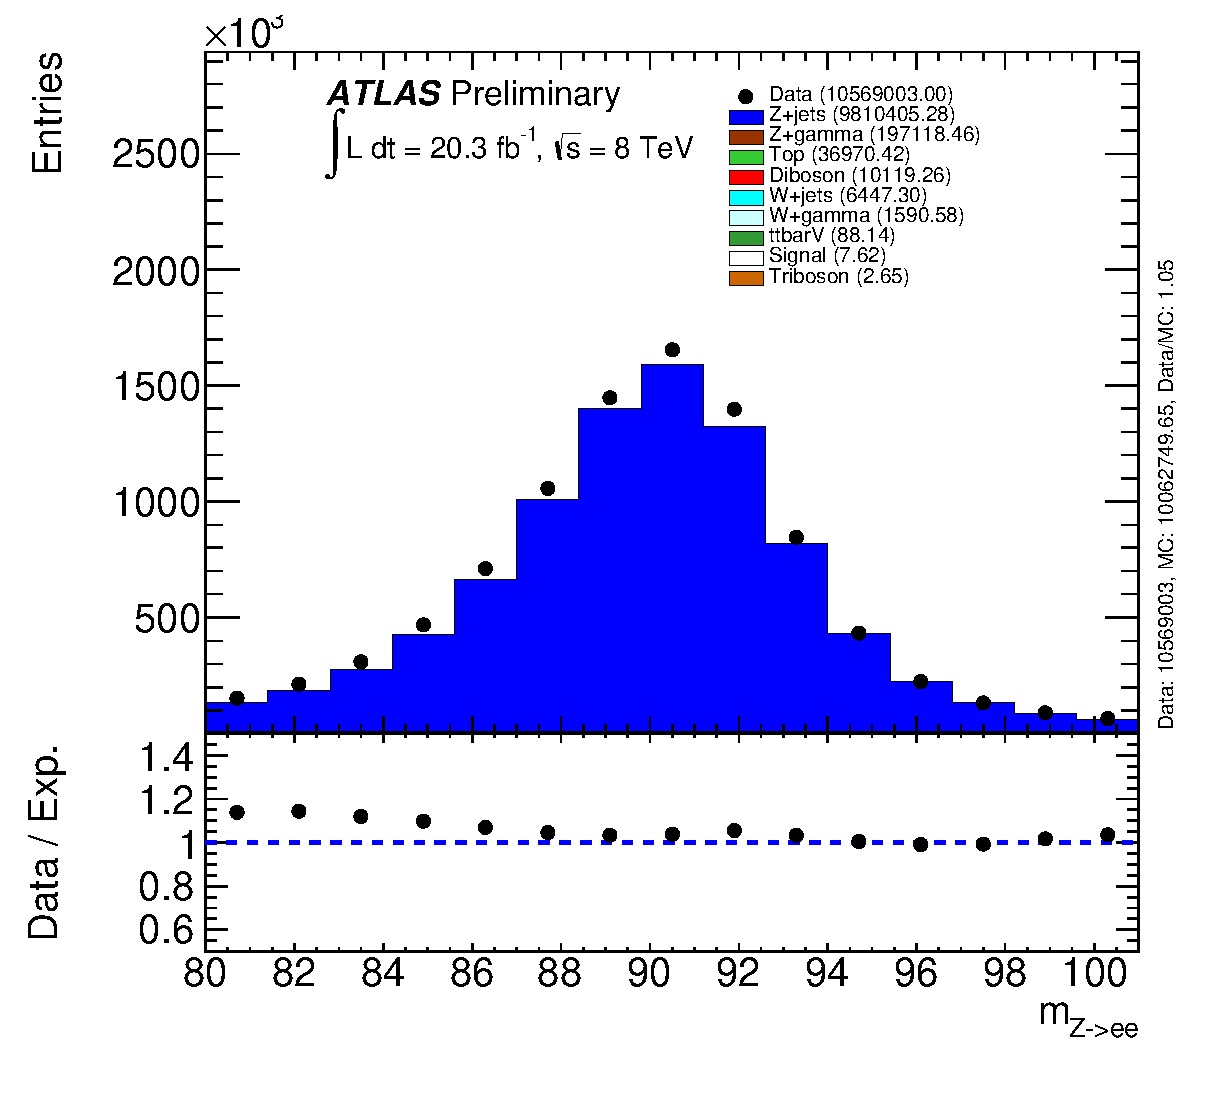
\includegraphics[width=0.4\columnwidth]{figures/fakes_bkg/CRs/hPtElectronZBosonloosecut_total_new.eps}
}
\centering
\subfigure{
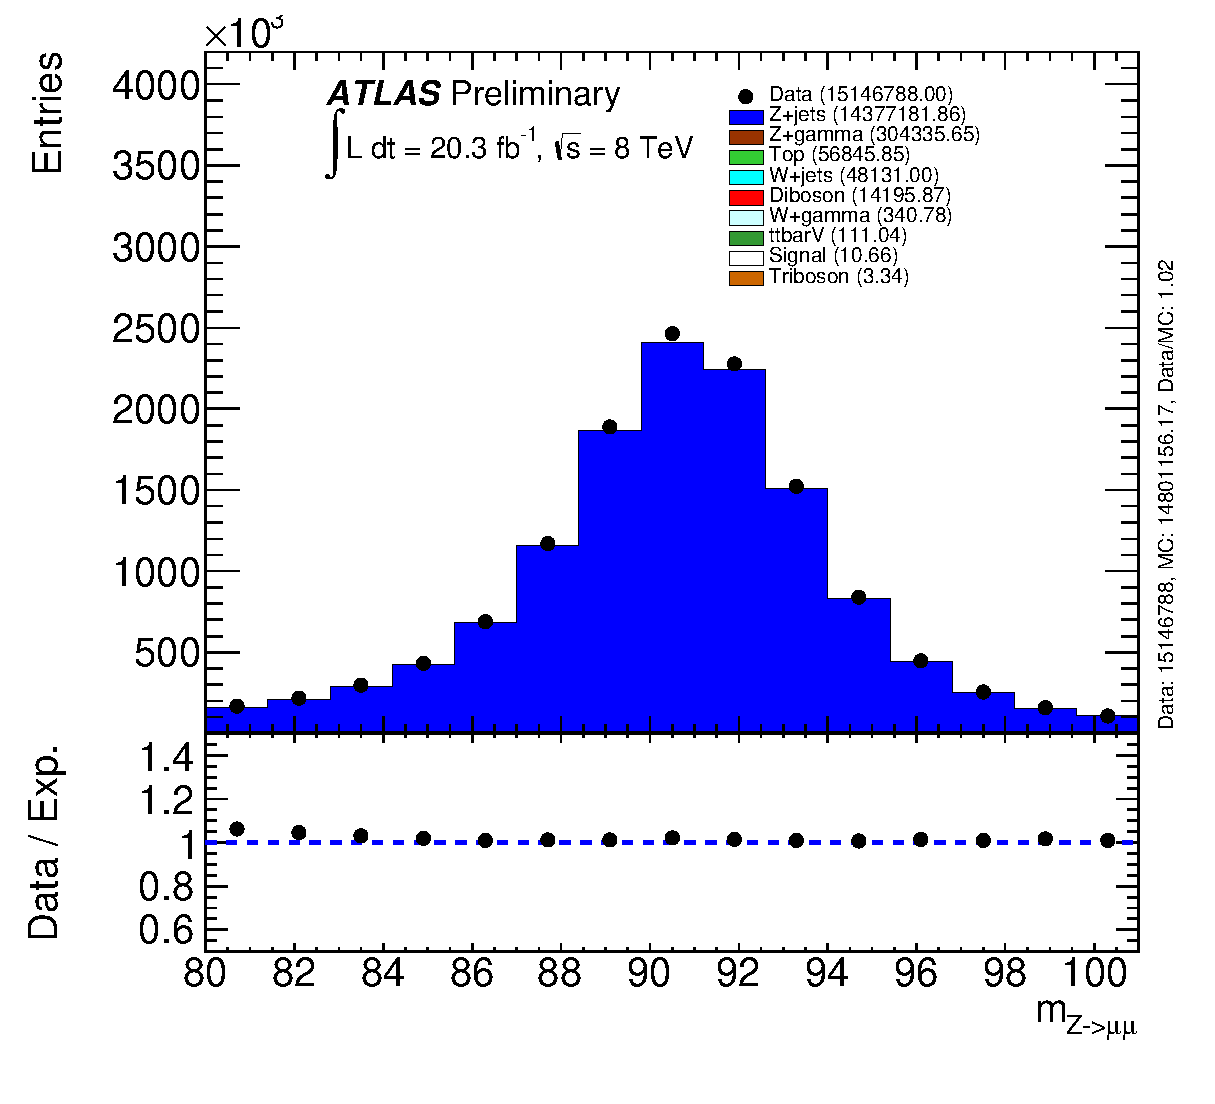
\includegraphics[width=0.4\columnwidth]{figures/fakes_bkg/CRs/hPtMuonZBosonloosecut_total_new.eps}
}
\vspace{-10mm}\caption{Invariant mass distribution of two opposite charge and same flavor di-lepton invariant mass electrons (left) and muons (right).}
\label{fig:realEff_CRs}
\end{figure}


\begin{figure}[h!]
\centering
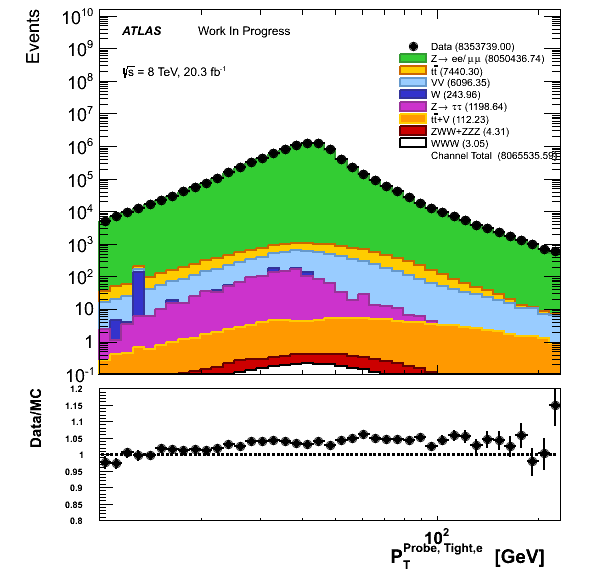
\includegraphics[width=0.4\columnwidth]{figures/fakes_bkg/CRs/RealTP/ProbeTightElectronPt_histratio.png}
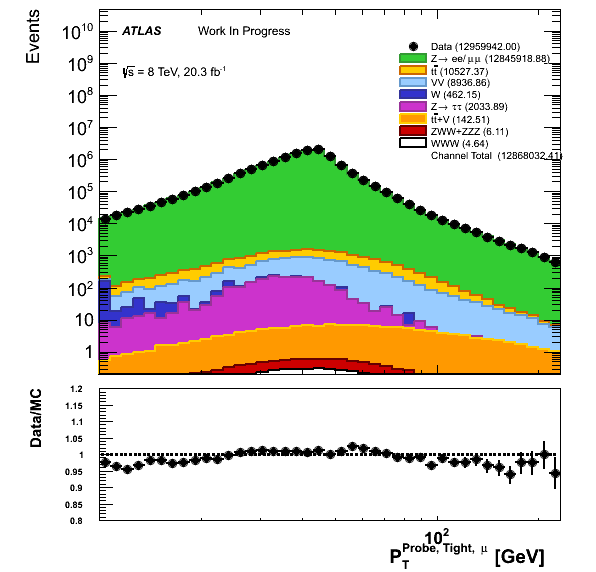
\includegraphics[width=0.4\columnwidth]{figures/fakes_bkg/CRs/RealTP/ProbeTightMuonPt_histratio.png}
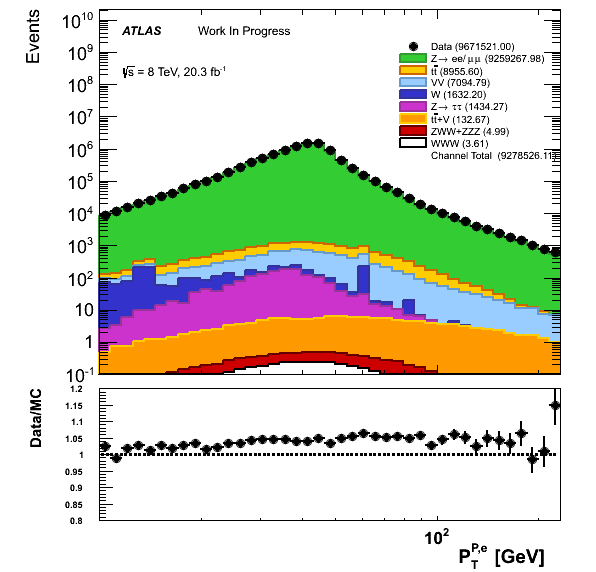
\includegraphics[width=0.4\columnwidth]{figures/fakes_bkg/CRs/RealTP/ProbeElectronPt_histratio.png}
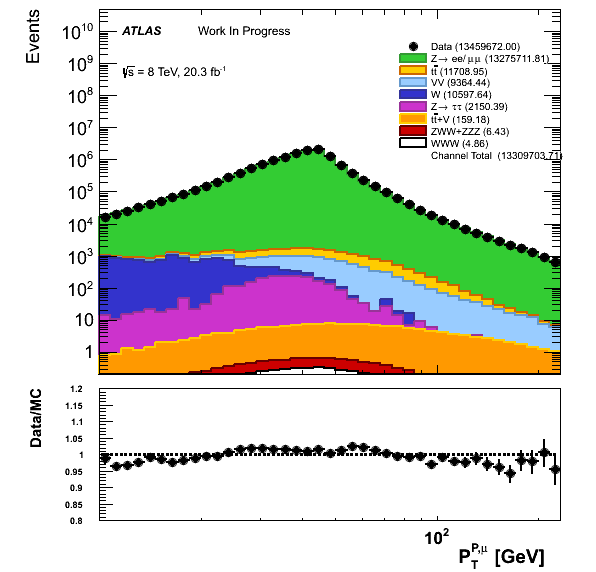
\includegraphics[width=0.4\columnwidth]{figures/fakes_bkg/CRs/RealTP/ProbeMuonPt_histratio.png}
\caption{Probe lepton \pt\ distributions in SFOS tag and probe control regions used to derive real rates.  Electron (left) and muon (right) are shown
when the probe lepton is either tight (top) or no additional selection (besides the pre-selection) is required (bottom)}
\label{fig:realEff_CRsPt}
\end{figure}


\begin{figure}[h!]
\centering
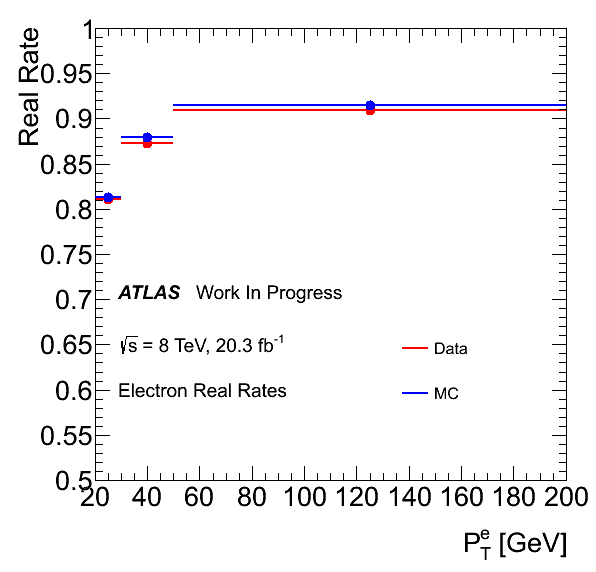
\includegraphics[width=0.45\columnwidth]{figures/fakes_bkg/Efficiencies/ElectronRealRates.png}
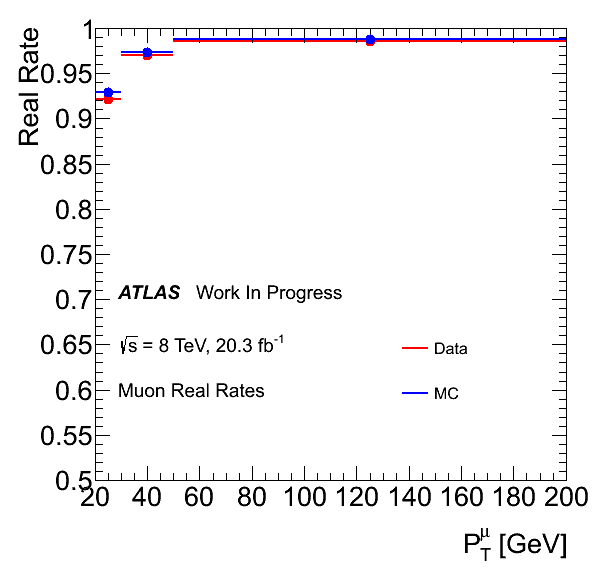
\includegraphics[width=0.45\columnwidth]{figures/fakes_bkg/Efficiencies/MuonRealRates.png}
\caption{Real lepton efficiency as a function of \pt\ and measured in data (red) and MC (blue) for electrons (left) and muons (right).}
\label{fig:realEff}
\end{figure}

\clearpage

%\tabcolsep=0.11cm
\begin{table}[h!]
\centering
\begin{tabular}{|l||c|c||c|c||c|}
\hline
&\multicolumn{2}{c||}{Data}&\multicolumn{2}{c||}{MC}&\multicolumn{1}{c|}{}\\ & $\varepsilon_r$ & $\sigma_{stat}$ & $\varepsilon_r$ & $\sigma_{stat}$ & $\sigma_{sys}$\\ 
\hline\hline
%$p_{T}\in[10,15]$ GeV &  $0.6285$ &  $0.0034$ &  $0.6420$ &  $0.0036$ &  $0.0135$\\ 
%$p_{T}\in[15,20]$ GeV &  $0.6960$ &  $0.0024$ &  $0.7056$ &  $0.0025$ &  $0.0096$\\ 
$p_{T}\in[20,30]$ GeV &  $0.8105$ &  $0.0011$ &  $0.8134$ &  $0.0013$ &  $0.0028$\\ 
$p_{T}\in[30,50]$ GeV &  $0.8732$ &  $0.0005$ &  $0.8794$ &  $0.0006$ &  $0.0062$\\ 
$p_{T} > 50$ GeV &  $0.9097$ &  $0.0012$ &  $0.9150$ &  $0.0012$ &  $0.0053$\\ 
\hline
\end{tabular}

\caption{Measured real efficiencies for electrons including statistical and systematic absolute uncertainties. 
Systematic is calculated by taking the difference
between the efficiencies measured in data and MC.  The efficiency measured in data is used as the nominal central value.
} 
\label{table:realEff_El}
\end{table} 

%\tabcolsep=0.11cm
\begin{table}[h!]
\centering
\begin{tabular}{|l||c|c||c|c||c|}
\hline
&\multicolumn{2}{c||}{Data}&\multicolumn{2}{c||}{MC}&\multicolumn{1}{c|}{}\\ & $\varepsilon$ & $\sigma_{stat}$ & $\varepsilon$ & $\sigma_{stat}$ & $\sigma_{sys}$\\ 
\hline\hline
%$p_{T}\in[10,15]$ GeV &  $0.8684$ &  $0.0033$ &  $0.8763$ &  $0.0036$ &  $0.0079$\\ 
%$p_{T}\in[15,20]$ GeV &  $0.8906$ &  $0.0024$ &  $0.8956$ &  $0.0025$ &  $0.0050$\\ 
$p_{T}\in[20,30]$ GeV &  $0.9217$ &  $0.0010$ &  $0.9291$ &  $0.0012$ &  $0.0074$\\ 
$p_{T}\in[30,50]$ GeV &  $0.9700$ &  $0.0004$ &  $0.9737$ &  $0.0006$ &  $0.0038$\\ 
$p_{T} > 50$ GeV &  $0.9862$ &  $0.0011$ &  $0.9878$ &  $0.0011$ &  $0.0017$\\ 
\hline
\end{tabular}

\caption{Measured real efficiencies for muons including statistical and systematic absolute uncertainties.
Systematic is calculated by taking the difference
between the efficiencies measured in data and MC.  The efficiency measured in data is used as the nominal central value.
} 
\label{table:realEff_Mu}
\end{table} 


\clearpage

\subsubsection{Fake lepton efficiency}

The fake efficiency represents the probability that a fake lepton satisfying the preselected criteria passes also the signal requirements. 
The measurement, performed separately for each $\pt$ bin, $i$, is performed in fake-enriched samples by looking at the number of probe leptons in data 
passing pre-selection, $n_i$, and comparing to the number which only pass also the tight
selection, $n^{Tight}_i$. Contamination from real leptons, $n^{\mathrm{Real}}_i$ and $n^{\mathrm{Tight}, \mathrm{Real}}_i$, 
and from photon converted leptons, $n^{\mathrm{PC}}_i$ and $n^{\mathrm{Tight},\mathrm{PC}}_i$, 
is corrected using MC by subtracting from the totals.  The rate is then determined as follows:
%\begin{align*}
\begin{equation}
\zeta_i=\frac{n^{\mathrm{Tight}}_i-n^{\mathrm{Tight},\mathrm{Real}}_i-n^{\mathrm{Tight},\mathrm{PC}}_i} {n_i -n^{\mathrm{Real}}_i -n^{\mathrm{PC}}_i }
\label{eq:fakerate}
\end{equation}
%\end{align*}
Since the rates depend on the fake lepton origin, the derivation is done separately for electrons and muons.     

The classification of leptons in MC as being either real or from photon conversion is performed on an event-by-event basis at truth level using the MCTruthClassifier tool~\cite{MCtruthclassifier:twiki}.  
Since this is a di-lepton control region, the majority of events with a real lepton
tag and a probe lepton due to photon conversion comes from the $W\gamma$ process where the photon converted lepton is an electron.
As expected, the number of probe muons coming from photon conversion are observed to be negligible.

Efficiencies are measured from a data set enriched with one tight lepton that passes the signal lepton selections with \pt$>40$~\GeV\ and 
one fake candidate satisfying only the pre-selection criteria defined in tables~\ref{tab:eledef} and~\ref{tab:muondef}. Events with additional loose or tight leptons are rejected. 
The QCD background may also enter these control regions, especially in low \met\ . Therefore, an additional \met$>10$~\GeV\ requirement is introduced. 
In order to reduce the contamination from real processes like $t\bar{t}$, $WW$ and $Z$, the two leptons are required to have the same sign.
Finally, the control regions are split based on the flavor of the tag and probe leptons.  The muon rates are determined in the region
with two muons while the electron rates are determined in the region with a muon tag and an electron probe.  The choice of a muon tag 
in the region used to derive the electron rates is particularly important since allowing electron tags have a large contamination from $Z$ backgrounds.
This is true even after the same-sign requirement because of charge mis-identification.  
The charge mis-identification rate for muons is negligible
and so allows one to use the muon-muon control region for the muon rates, which has the least contamination.
This behavior can be seen in the distributions of probe muon transverse momentum in the same-sign muon-muon tag-and-probe control region used to derive
the muon fake rates shown in Fig.~\ref{fig:fakeEff_CRs_muon} while
the distributions of probe electron transverse momentum are shown in the same-sign electron-muon tag-and-probe control region used to derive
the electron fake rates shown in Fig.~\ref{fig:fakeEff_CRs_electron}.
The control regions for both electrons and muons are further split based on the number of b-tagged jets in the event, 
which has an effect on the source of the fake leptons.  In particular, requiring b-tagged jets increases the fraction
of fake leptons coming from heavy flavor. Two different sets of control regions were ultimately considered, those
with at least one b-tagged jet and those without any requirement on the presence of b-tagged jets.  The region
with at least one b-tagged jet ($N_{b-jet} > 0$) is used as the central value since it contains more heavy flavor contributions
and so compares better with the signal regions, as described later in Section~\ref{sec:fakecomposition}.  The other is used 
to determine a systematic on the composition, described later.  


A detailed breakdown of the numbers used to compute the fake rates are shown in Appendix~\ref{sec:appendix_fakebg}.
%would it be useful to show the other di-lepton control regions in an appendix?

Three systematic uncertainties are considered. First, the subtraction of the processes with 
two real leptons ($t\bar{t}V$, $VV$ and $VVV$) using MC prediction introduced an uncertainty on 
their cross-sections. This effect is estimated by varying the MC normalization by $\pm 20$\%.  %should rerun with 5%
We refer to this is as the 'correlated' systematic uncertainty.
Second, given that the extraction regions and the signal regions have different kinematic selections, 
the fake leptons of different origin dominate. This kinematic dependence of fake efficiencies has been estimated 
by modifying the requirements of the sample used for the measurement. In particular, the cut thresholds 
on the $E_{T}^{Miss}$ and tag lepton $\pt$ used
for determining the di-lepton control regions are varied. The $E_{T}^{Miss}$ threshold is 
varied in 5~GeV steps scanning a range of $\pm 10$~GeV around the nominal
threshold of $E_{T}^{Miss} > 10$~GeV while the $\pt$ threshold is varied in 5~GeV steps in a range of $\pm 20$~GeV 
around the nominal threshold of $\pt > 40$~GeV.  When varying the $E_{T}^{Miss}$ cut, the $\pt$ cut
is kept at the nominal threshold and vise-versa. This is referred to as the 'uncorrelated' systematic.
These are determined separately for electrons and muons, since they use different control regions. The 'uncorrelated' and
'correlated' systematics for electrons and muons are then combined together by adding in quadrature on an event-by-event basis.
As a result the uncertainty is presented as a single systematic uncertainty on the fake electron
contribution and a separate single systematic on the fake muon contribution.
The third and final systematic contribution comes from the choice of control region, based on the number of b-tagged
jets, as described earlier.  The nominal control regions for both the electron and muon cases is when 
there is at least one b-tagged jet present.  The difference between the rates for the nominal case
and the region where no requirement is placed on the presence of b-tagged jets is chosen as a systematic.
We have determined that the difference in the composition in these two regions adequately covers the difference
in composition that may be present due to the extrapolation from the control regions to the signal regions. This is 
discussed in more detail in Section~\ref{sec:fakecomposition}.  Another set of control regions was studied
which vetoes any b-tagged jets, but this was observed to give a very large difference in composition which is 
probably too conservative of an estimate to be used as a reasonable systematic.
The rates along with the statistical and systematic uncertainties are summarized in Fig.~\ref{fig:fakeEff} 
as well as in Tables \ref{table:fakeEff_El} and \ref{table:fakeEff_Mu}.
The final binning of the efficiency is chosen to be coarse enough
to have good statistics in the ratio while also preserving shape information as a function
of $\pt$. 


%\begin{figure}[h!]
%\centering
%\subfigure{
%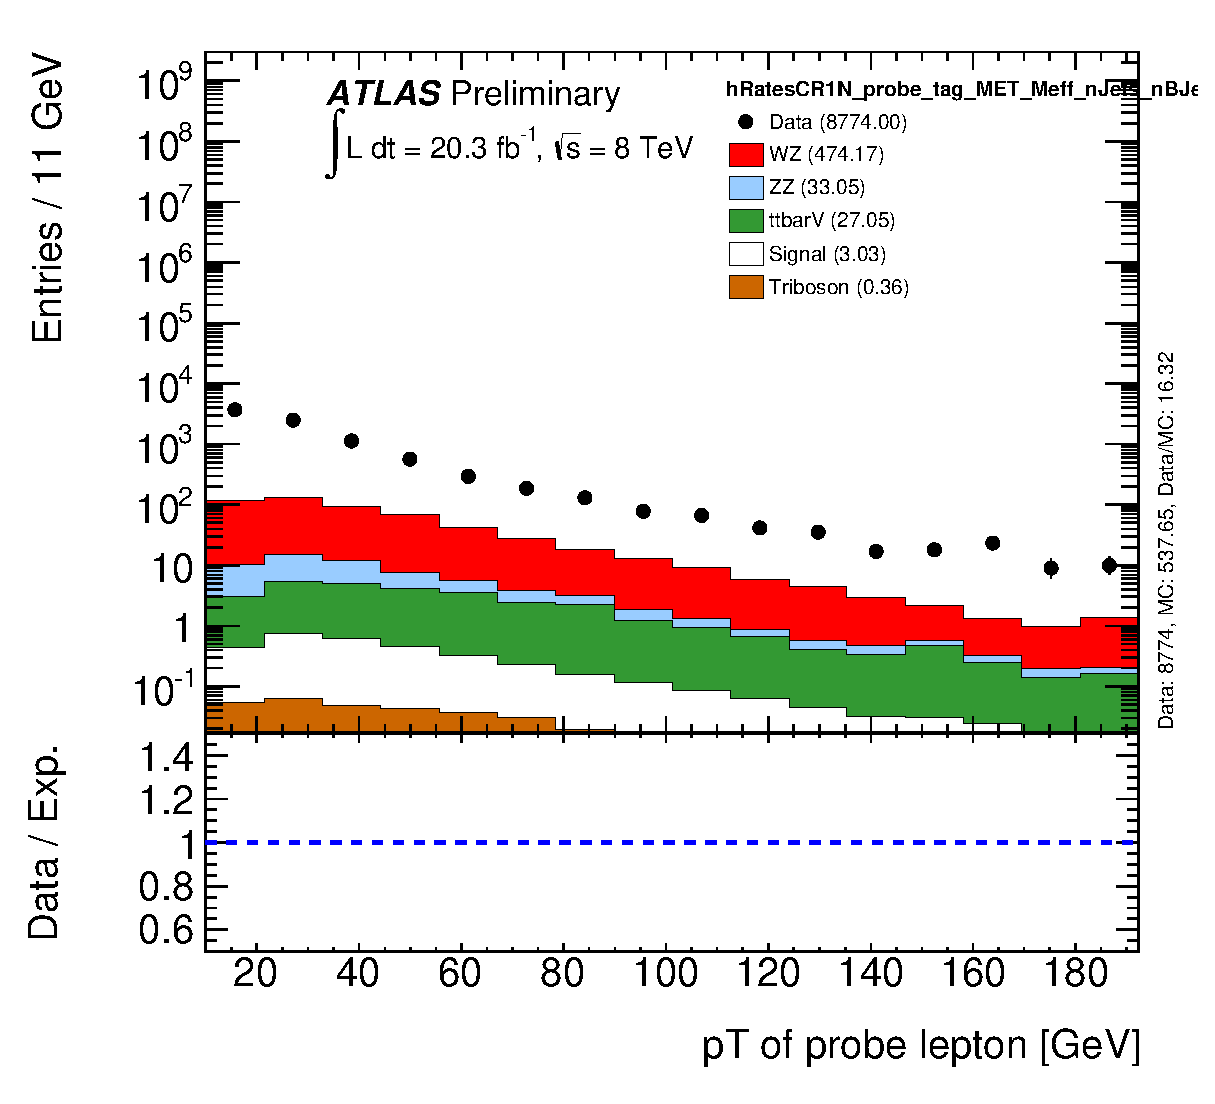
\includegraphics[width=0.3\columnwidth]{figures/fakes_bkg/CRs/CR1N_probePt_all_total.eps}
%}
%\centering
%\subfigure{
%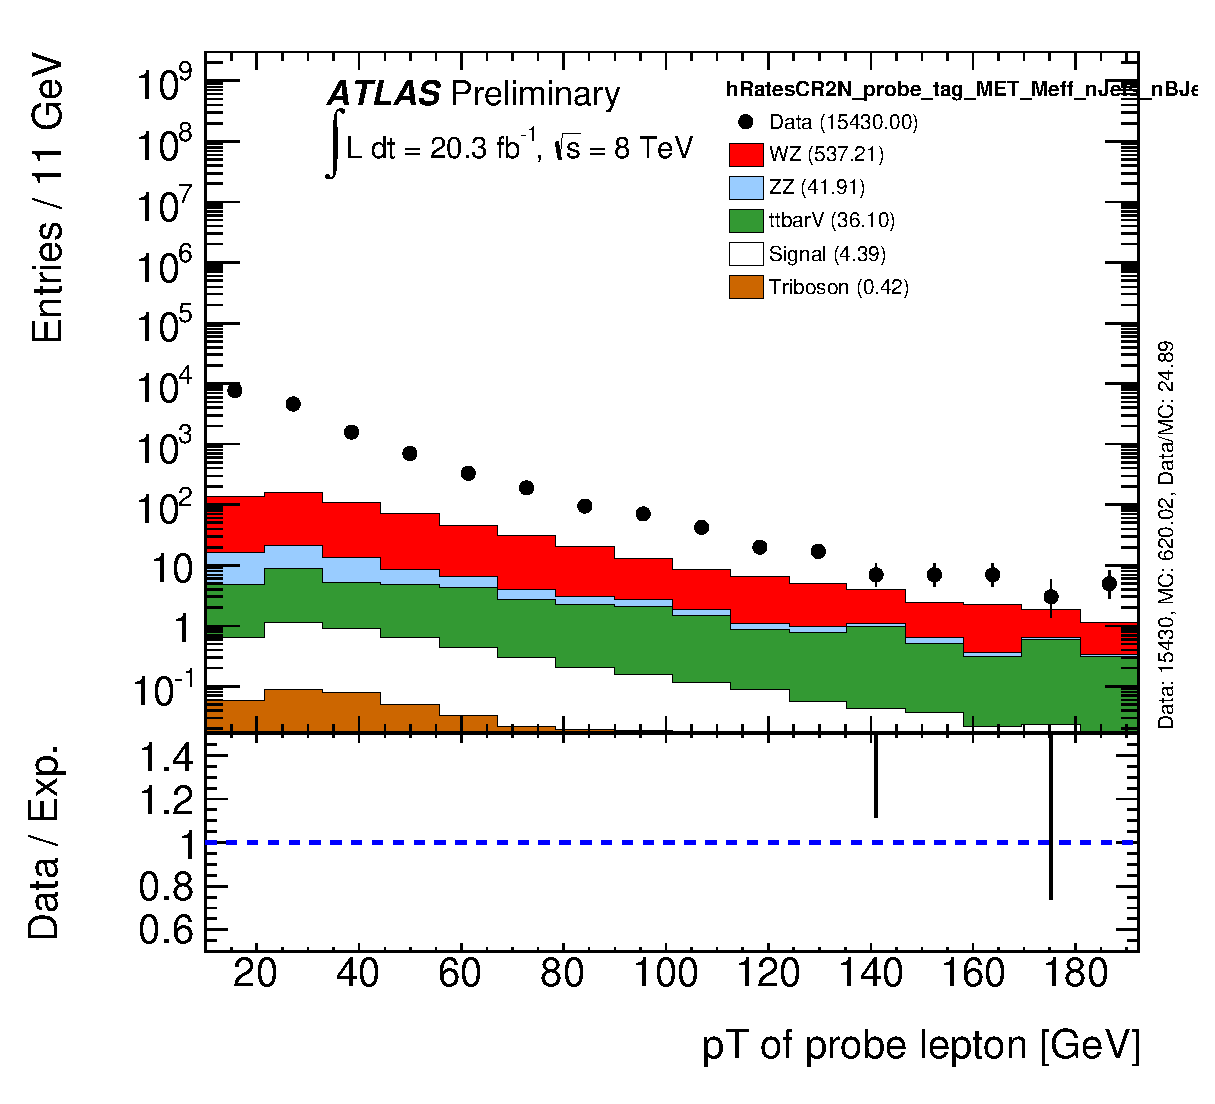
\includegraphics[width=0.3\columnwidth]{figures/fakes_bkg/CRs/CR2N_probePt_all_total.eps}
%}\\ 
%\vspace{-14mm}
%\subfigure{
%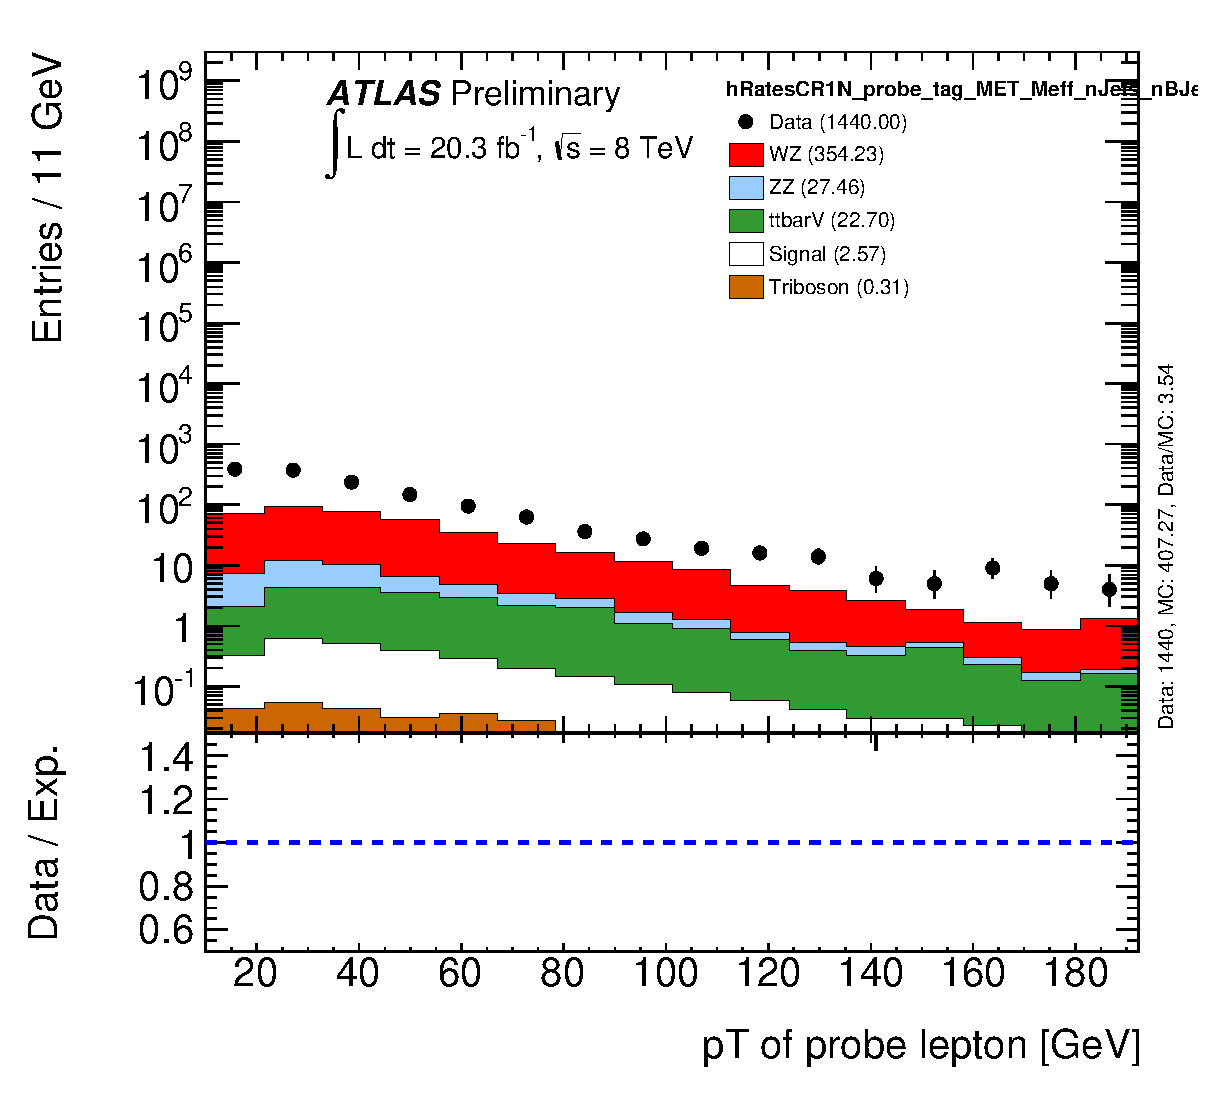
\includegraphics[width=0.3\columnwidth]{figures/fakes_bkg/CRs/CR1N_probePt_tight_total.eps}
%}
%\centering
%\subfigure{
%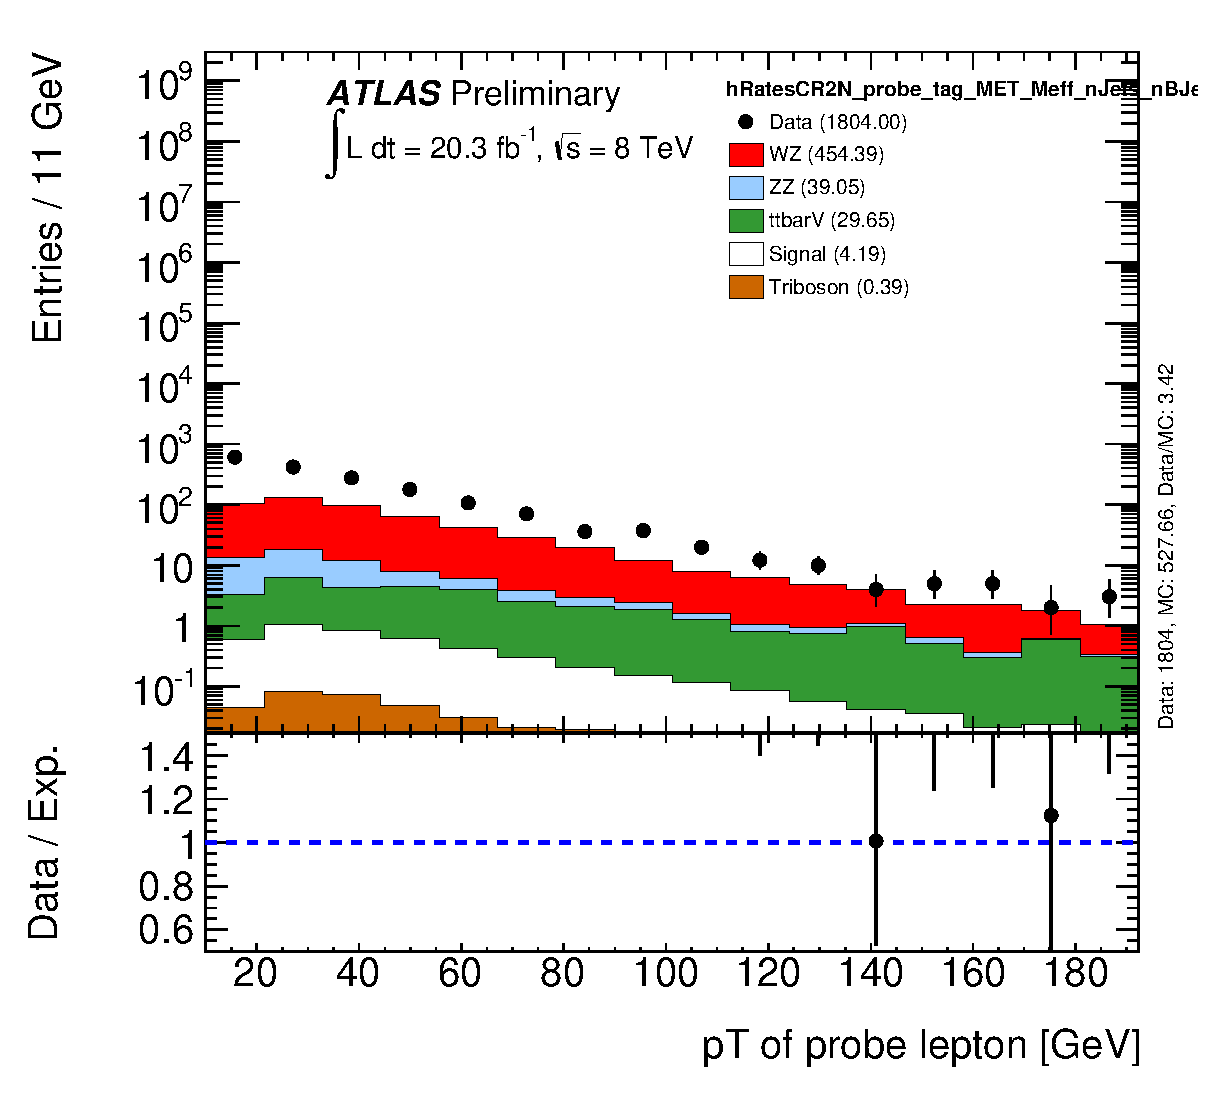
\includegraphics[width=0.3\columnwidth]{figures/fakes_bkg/CRs/CR2N_probePt_tight_total.eps}
%}
%\vspace{-10mm}\caption{Transverse momentum distributions \pt\ of probe electron (left) and muon (right) in the control regions. The probe passes pre-selection (top) and signal (bottom) criteria.}
%\label{fig:fakeEff_CRs}
%\end{figure}








\begin{figure}[ht!]
\centering
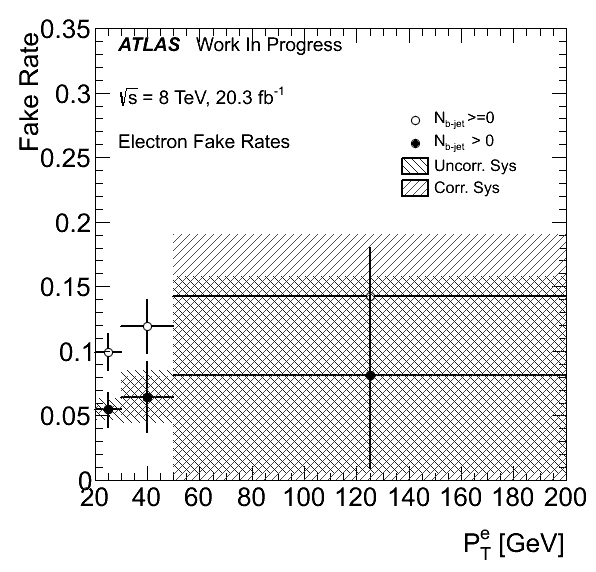
\includegraphics[width=0.45\columnwidth]{figures/fakes_bkg/Efficiencies/ElectronFakeRates.png}
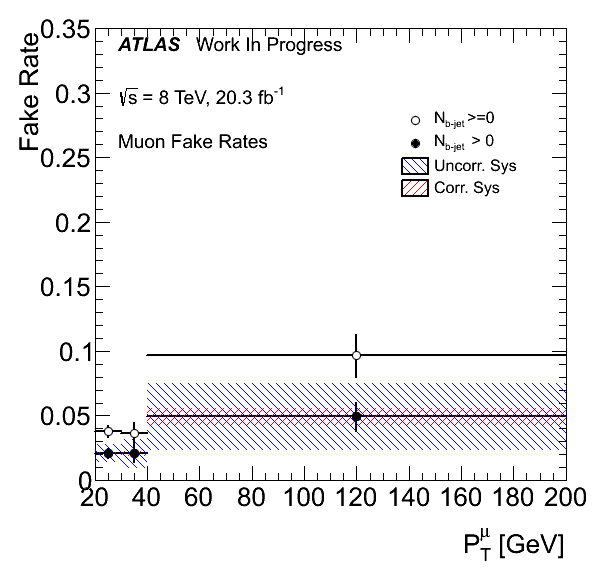
\includegraphics[width=0.45\columnwidth]{figures/fakes_bkg/Efficiencies/MuonFakeRates.png}
%\vspace{-10mm}
\caption{Distributions of the electron (left) and muon (right) fake rates as a function of \pt\ extracted in the control regions for three different selections: without any additional requirement on $b$-jets in the event and at least one $b$-jet.}
\label{fig:fakeEff}
\end{figure}




%\tabcolsep=0.1cm
%\begin{table}
%\centering
%\resizebox{0.8\textwidth}{!}{
%\begin{tabular}{l|c|c|c|c|c|c|c} 
%\hline
%\multicolumn{4}{c}{Electrons} &\multicolumn{4}{c}{Muons}\\ \hline
%\pt\ region & Fake eff. & $\sigma_{\mathrm{stat}}$ & $\sigma_{\mathrm{syst}}$ &\pt\ region & Fake eff. & $\sigma_{\mathrm{stat}}$ & $\sigma_{\mathrm{syst}}$ \\\hline
%$\pt \in [10, 15]$ \GeV\ & $0.$ & $0.$ & $0.$ 
%& $\pt \in [10, 15]$ \GeV\ & $0.$ & $0.$ & $0.$ \\
%$\pt \in [15, 30]$ \GeV\ & $0.$ & $0.$ & $0.$
%& $\pt \in [15, 20]$ \GeV\ & $0.$ & $0.$ & $0.$ \\
%$\pt\in [30, 50]$ \GeV\ & $0.$ & $0.$ & $0.$
%& $\pt\in [20, 40]$ \GeV\ & $0.$ & $0.$ & $0.$ \\
%$\pt > 50$ \GeV\ & $0.$ & $0.$ & $0.$
%& $\pt > 40$ \GeV\ & $0.$ & $0.$ & $0.$ \\
%\hline
%\end{tabular}  }
%\caption{Measured fake efficiencies for electrons and muons including statistical and systematic absolute uncertainties.} 
%\label{table:fakeEff_All}
%\end{table} 

\begin{table}[h]
\centering
\begin{tabular}{|l||c|c|c|c||c|c|c|c|}
\hline
 & $\zeta$ & $\sigma_{stat}$ & $\sigma_{sys}^{uncorr}$ & $\sigma_{sys}^{corr}$\\ 
\hline\hline
&\multicolumn{4}{c||}{$N_{b-jet} > 0$}\\ \hline
$p_{T}\in[20,30]$ GeV &  $0.0549$ &  $0.0136$ &  $0.0084$ &  $0.0032$\\ 
$p_{T}\in[30,50]$ GeV &  $0.0645$ &  $0.0272$ &  $0.0203$ &  $0.0161$\\ 
$p_{T} > 50$ GeV &  $0.0816$ &  $0.0723$ &  $0.0764$ &  $0.1088$\\ 
\hline\hline &\multicolumn{4}{c||}{$N_{b-jet} \geq 0$}\\ \hline
$p_{T}\in[20,30]$ GeV &  $0.0995$ &  $0.0141$ &  $0.0270$ &  $0.0099$\\ 
$p_{T}\in[30,50]$ GeV &  $0.1192$ &  $0.0208$ &  $0.0324$ &  $0.0232$\\ 
$p_{T} > 50$ GeV &  $0.1428$ &  $0.0374$ &  $0.0428$ &  $0.0674$\\ 
\hline
\end{tabular}

\caption{Measured fake efficiencies for electrons measured in three regions: with no additional requirements on the presence of $b$-jets and with at least one $b$-jet in a event. Statistical and systematic absolute uncertainties are also shown.} 
\label{table:fakeEff_El}
\end{table} 


\begin{table}[h]
\centering
\begin{tabular}{|l||c|c|c|c||c|c|c|c|}
\hline
 & $\zeta$ & $\sigma_{stat}$ & $\sigma_{sys}^{uncorr}$ & $\sigma_{sys}^{corr}$\\ 
\hline\hline
&\multicolumn{4}{c||}{$N_{b-jet} > 0$}\\ \hline
$p_{T}\in[20,30]$ GeV &  $0.0208$ &  $0.0037$ &  $0.0067$ &  $0.0009$\\ 
$p_{T}\in[30,40]$ GeV &  $0.0207$ &  $0.0066$ &  $0.0113$ &  $0.0020$\\ 
$p_{T} > 40$ GeV &  $0.0492$ &  $0.0109$ &  $0.0259$ &  $0.0068$\\ 
\hline\hline &\multicolumn{4}{c||}{$N_{b-jet} \geq 0$}\\ \hline
$p_{T}\in[20,30]$ GeV &  $0.0378$ &  $0.0046$ &  $0.0140$ &  $0.0040$\\ 
$p_{T}\in[30,40]$ GeV &  $0.0360$ &  $0.0091$ &  $0.0096$ &  $0.0089$\\ 
$p_{T} > 40$ GeV &  $0.0967$ &  $0.0166$ &  $0.0252$ &  $0.0244$\\ 
\hline
\end{tabular}

\caption{Measured fake efficiencies for muons measured in three regions: with no additional requirements on the presence of $b$-jets and with at least one $b$-jet in the event.  Statistical and systematic absolute uncertainties are also shown.} 
\label{table:fakeEff_Mu}
\end{table} 


\clearpage

\subsubsection{Study of the fake lepton composition}
\label{sec:fakecomposition}

The use of the generalized matrix method to determine the 
relies on the assumption that the 
fake rates derived in the di-lepton control regions may be extrapolated to the three lepton signal regions.  
The fake rate depends primarily on the source of the fake leptons, thus
one can check the validity of this assumption by looking at the composition of the
different fake lepton sources in the di-lepton control regions and comparing 
them to the
composition in the three lepton signal regions. 

The fake composition is investigated by classifying the MC events as a function of the origin of the fake leptons found in each event.  The MCTruthClassifier tool~\cite{MCtruthclassifier:twiki} is used
to identify the fake laptops origin as follows:

\begin{itemize}
\item Real - Prompt leptons
		\begin{itemize}
		\item \emph{IsoElectron} 
		\item \emph{IsoMuon}
		\item In $Z\gamma$ events classified as either \emph{UnknownElectron} or \emph{UnknownMuon} and parent of lepton is $\gamma$.
		\item In $Z\rightarrow\tau\tau$ events classified as either \emph{NonIsoElectron} or \emph{NonIsoMuon} and lepton has $\tau$ as parent.
		\end{itemize}
\item Heavy Flavor (HF) - Leptons from heavy flavor jets or heavy hadron decays
		\begin{itemize}
		\item \emph{NonIsoElectron} 
		\item \emph{NonIsoMuon}
		\end{itemize}
\item Light Flavor (LF) -  Leptons from light flavor jets
		\begin{itemize}
		\item \emph{Hadron} 
		\item \emph{Others}
		\item In $ZWW$ and $ZZZ$ events classified as either \emph{UnknownElectron} or \emph{UnknownMuon} and parent of lepton is either an up quark, down quark, or a gluon.
		\end{itemize}
\item Photon Conversion (PC)  - Leptons due to radiation
		\begin{itemize}
		\item \emph{BkgElectron} 
		\item \emph{BkgMuon}
		\end{itemize}

\end{itemize}

The composition is shown for electrons in the di-lepton control 
regions in Table~\ref{table:CompositionElectronCR} and in the event pre-selection and in region close to the signal regions in Table~\ref{table:CompositionElectronSR}.
First, one can see that the PC contribution is roughly half of the fake contribution
estimate using MC
in the control regions and in the region close to the signal regions. Since this is being estimated
using MC close to the signal regions, 
this component is subtracted out in order to remove any double counting
in the final estimate. Then, after subtraction,
if one compares the composition in the control regions
to the composition in the region close to the signal regions only for electrons, 
in particular after tight selection, one can see that 
the composition is similar for both, 
with about 50 to 75 \% coming from HF and the rest from LF.

For the muons, one can see the composition in the di-lepton control regions in 
Table~\ref{table:CompositionMuonCR} and in the event pre-selection
and region close to the signal regions in Table~\ref{table:CompositionMuonSR}. For the muons the PC
component is negligible, as expected, and there is no need for subtraction.
In this case, the composition is dominated by HF, contributing about 90\% with the
rest coming from LF.  This is true in the region close to the signal regions and in the control regions.

The differences observed in the composition between the inclusive $b-jet$ and $b-jet$ 
tagged di-lepton control regions is observed to be of a similar size
to the difference in the composition for the region close to the signal regions for both the electron 
and muon cases.
Thus, comparing the rates derived in the control regions using the two different
$b-jet$ criteria should take into account any differences in the composition due
to extrapolation. This is the motivation for choosing the difference in these two 
control regions as an additional systematic on the fake rates.

Using this study of the composition, we conclude that the composition appears to be
consistent between the control regions and the region close to the signal regions.  We have chosen 
a comparison of two different di-lepton control regions to be used a systematic
which should take into account any remaining differences in the composition.

It should be said that in the di-lepton control regions, 
the MC estimate strongly underestimates the amount observed
in data, presumably because of additional sources of fakes 
not modeled in our MC, such as from QCD. 
The difference in the estimates can be clearly seen in Figures~\ref{fig:fakeEff_CRs_muon_stacked}
and \ref{fig:fakeEff_CRs_electron_stacked} which show the stacked MC estimate from real, photon conversion,
heavy flavor and light flavor sources compared to data.
Thus, the composition estimates shown are only reliable 
if these additional sources would have a similar composition to the ones observed
in this study that we are able to model. This effectively 
puts a large uncertainty on the composition estimates observed in this study. Also,
because the additional sources are most likely dominated by QCD, the PC 
contribution to these sources should be small. Thus, the PC component before subtraction
is likely overstated as shown in 
Tables~\ref{table:CompositionElectronCR} 
and \ref{table:CompositionElectronSR}.
As discussed earlier, we subtract the PC
component from the data when obtaining the fake rate. This procedure then assumes
explicitly that all of the photon conversion contribution is modeled in MC and is 
small.


\begin{figure}[h!]
\centering
\subfigure{
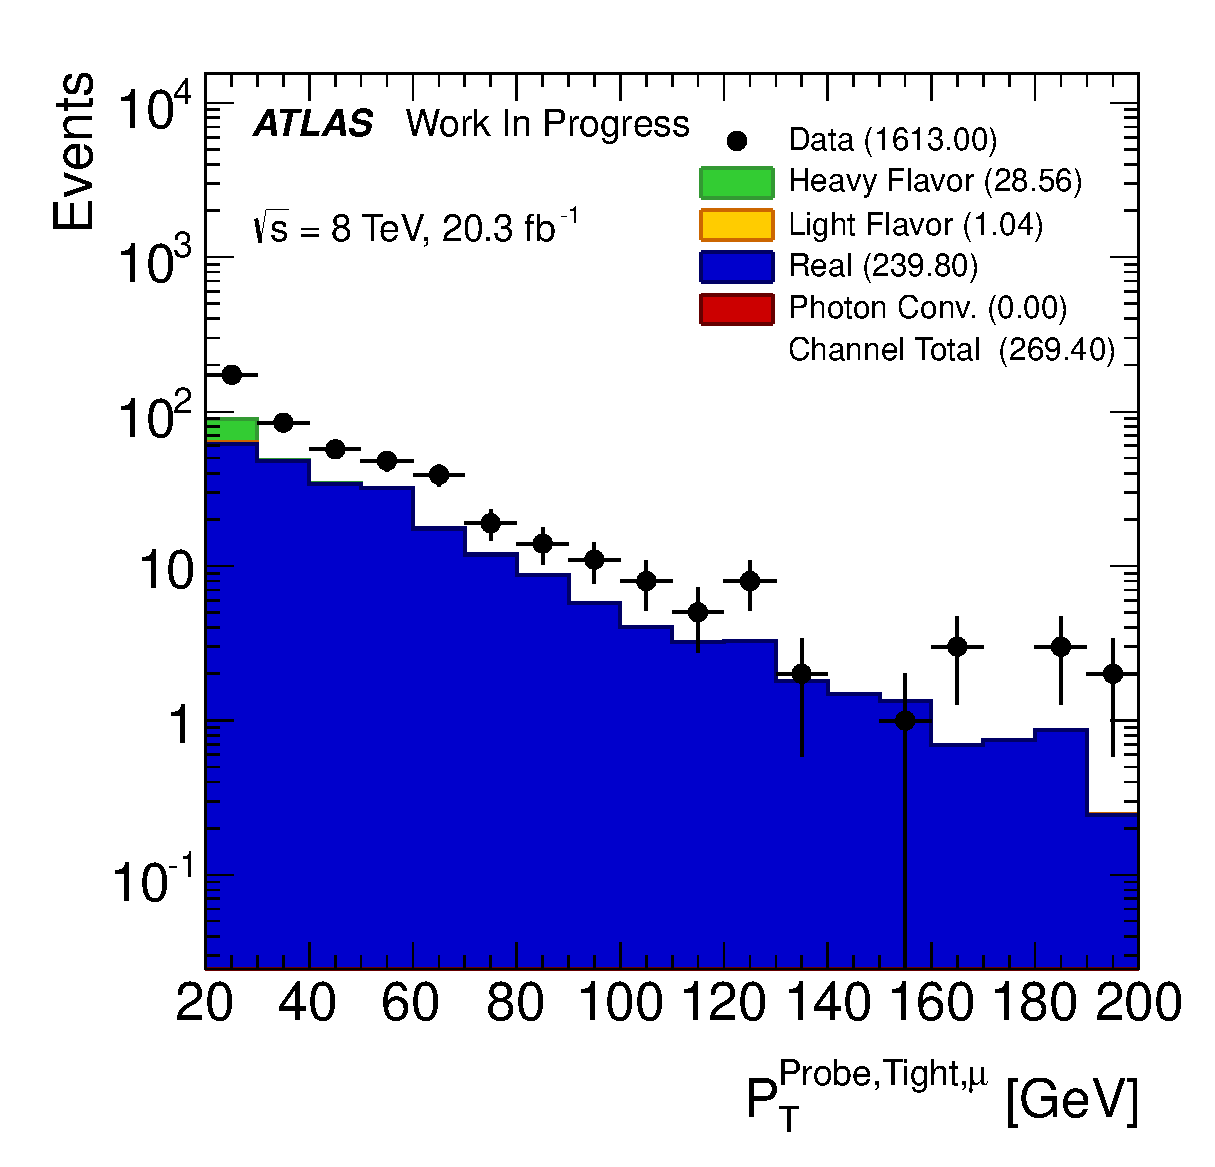
\includegraphics[width=0.45\columnwidth]{figures/fakes_bkg/CRs/SameSignMuonMuon/Stacked/ProbeTightMuonPt.eps}
}
%\centering
%\subfigure{
%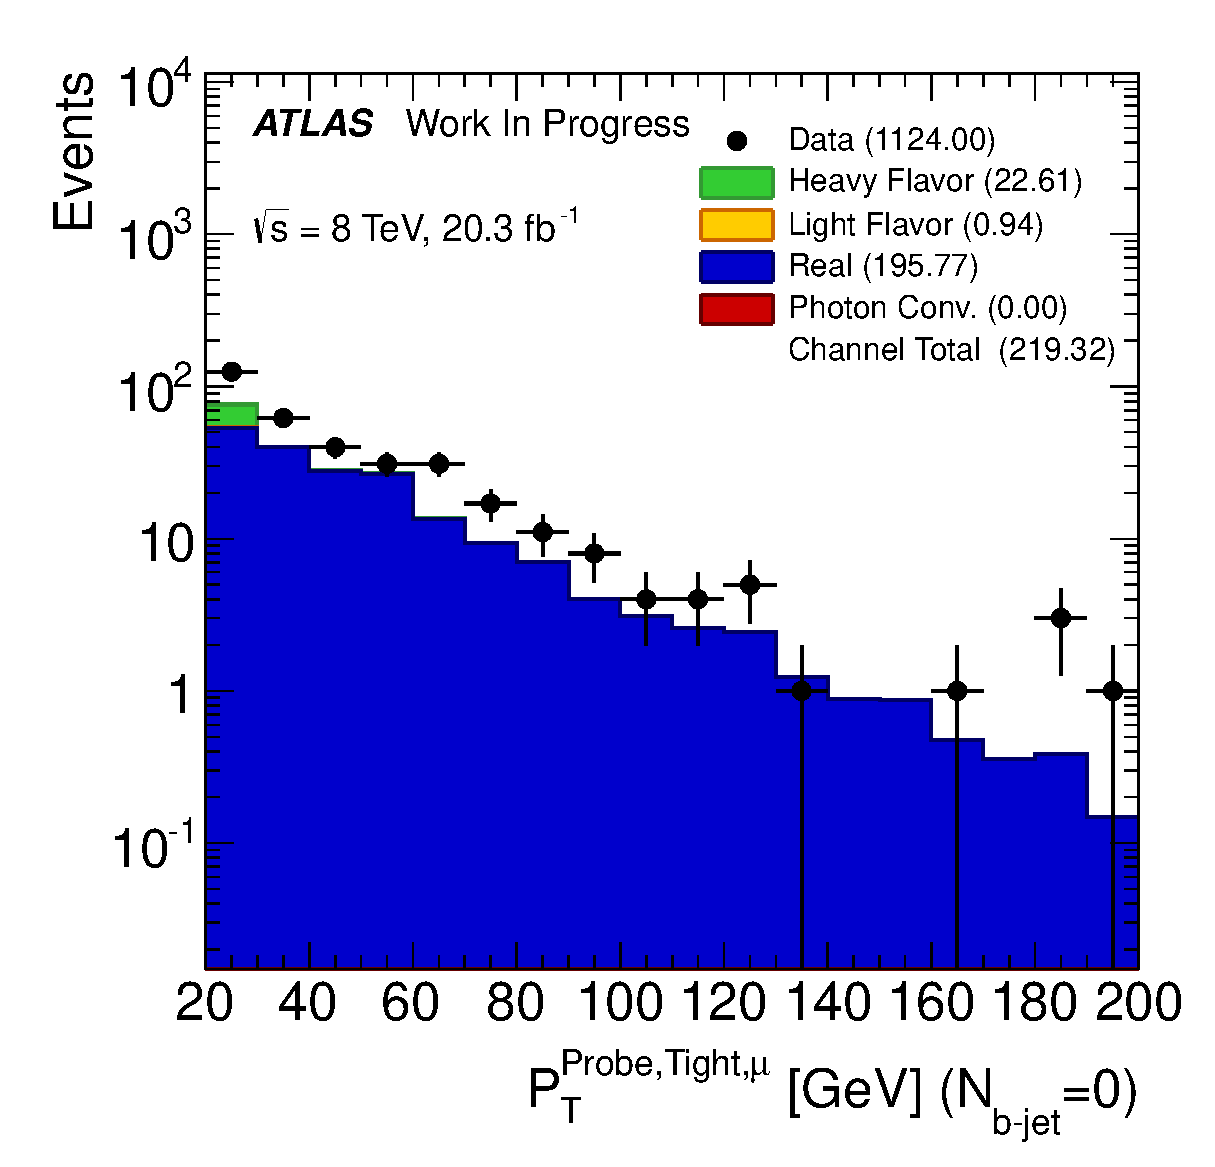
\includegraphics[width=0.3\columnwidth]{figures/fakes_bkg/CRs/SameSignMuonMuon/Stacked/ProbeTightMuonPtBJetEq0.eps}
%}
\centering
\subfigure{
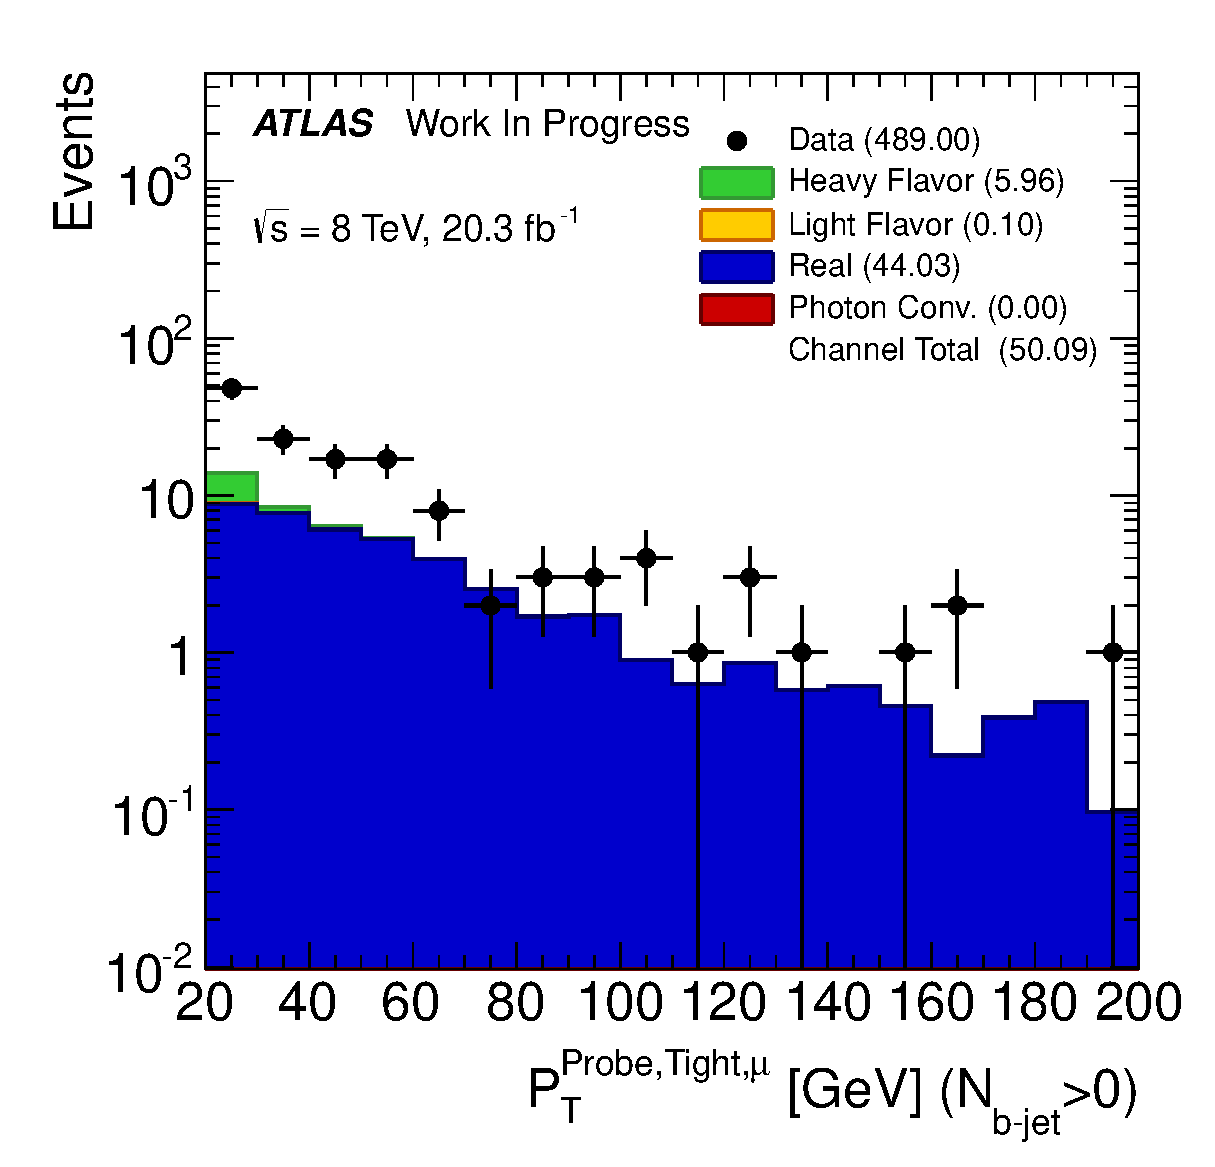
\includegraphics[width=0.45\columnwidth]{figures/fakes_bkg/CRs/SameSignMuonMuon/Stacked/ProbeTightMuonPtBJetGt0.eps}
}
%\vspace{-1mm}
\centering
\subfigure{
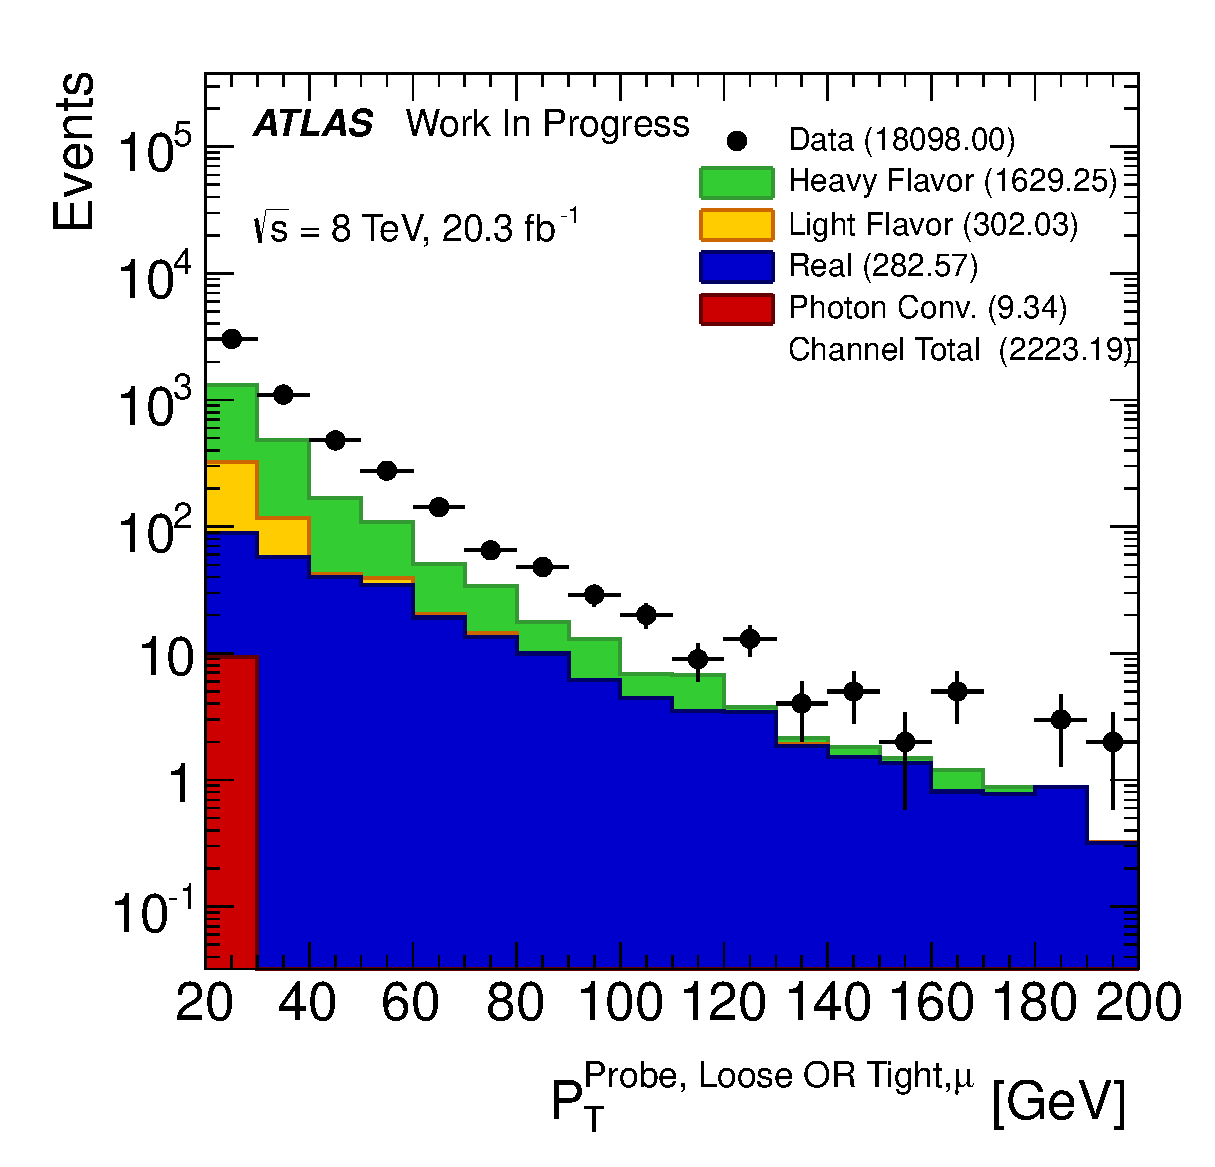
\includegraphics[width=0.45\columnwidth]{figures/fakes_bkg/CRs/SameSignMuonMuon/Stacked/ProbeLooseORTightMuonPt.eps}
}
%\centering
%\subfigure{
%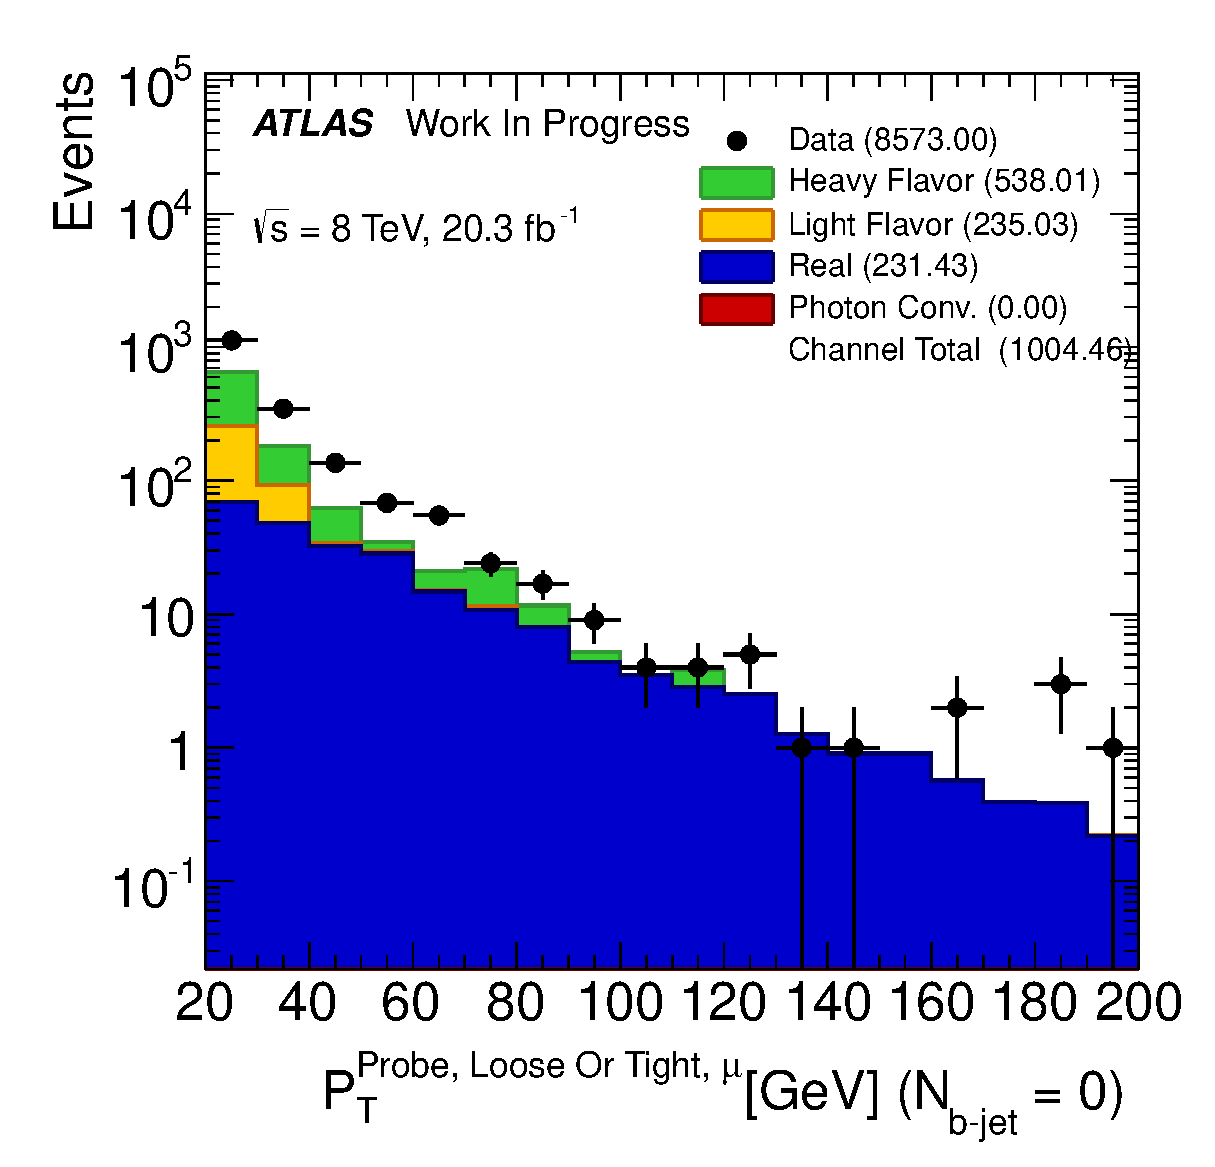
\includegraphics[width=0.45\columnwidth]{figures/fakes_bkg/CRs/SameSignMuonMuon/Stacked/ProbeLooseORTightMuonPtBJetEq0.eps}
%}
\centering
\subfigure{
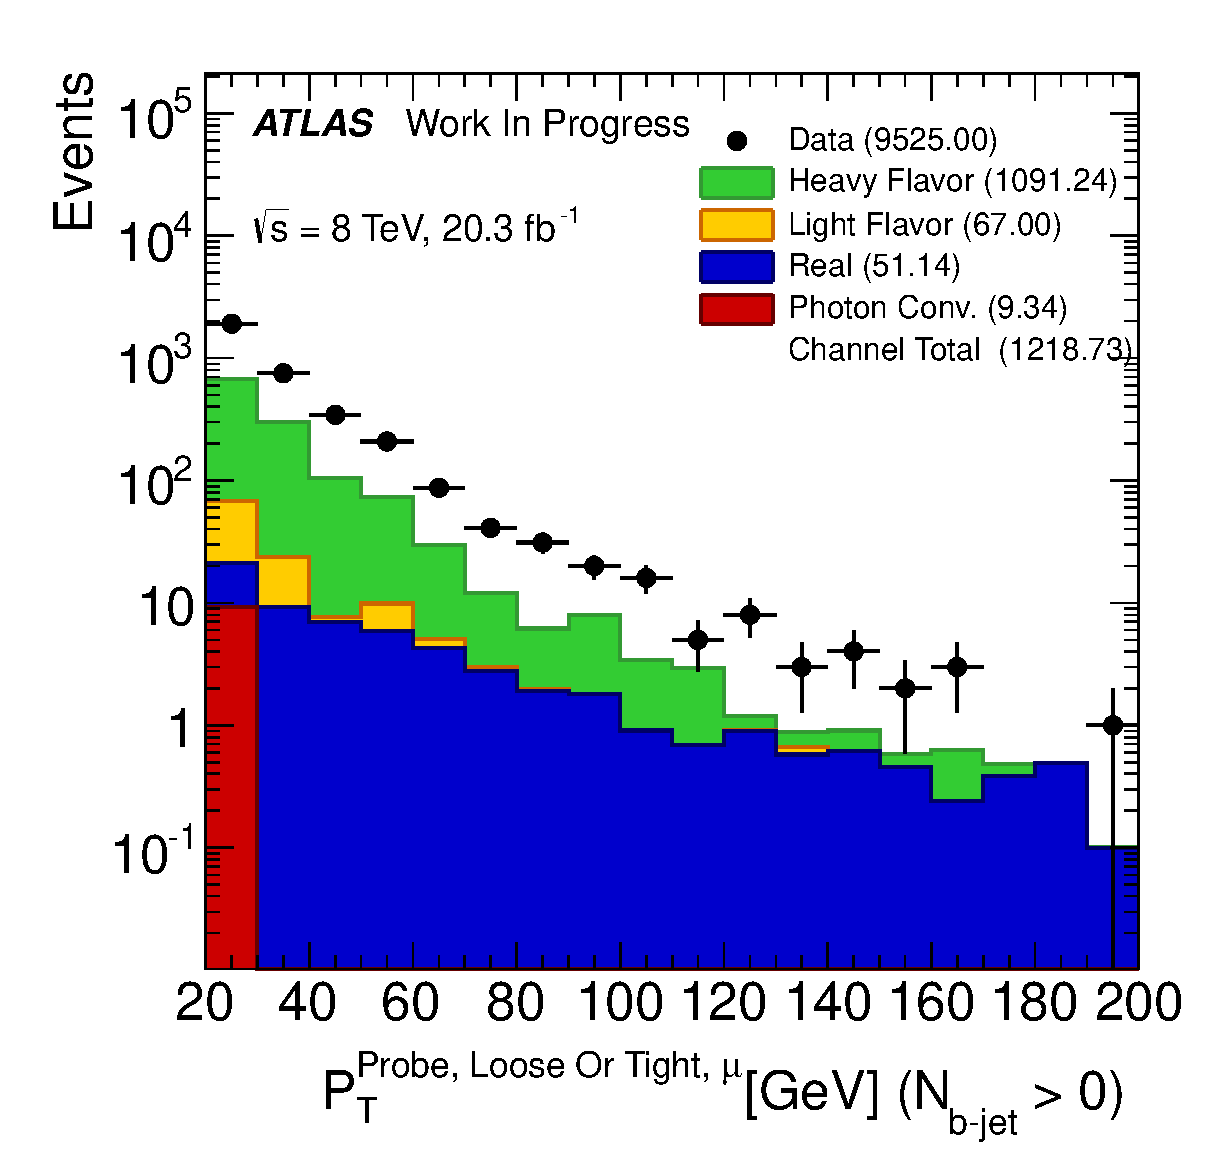
\includegraphics[width=0.45\columnwidth]{figures/fakes_bkg/CRs/SameSignMuonMuon/Stacked/ProbeLooseORTightMuonPtBJetGt0.eps}
}
\vspace{-10mm}\caption{Transverse momentum distributions \pt\ of tight probe muons (top) and loose OR tight probe muons (bottom) passing signal selection criteria in the control Same-Sign $\mu-\mu$ control region without any additional requirement on $b$-jets in the event (left) and at least one $b$-jet (right). 
The amount observed in data (black points) corresponds to $n$ (bottom) and $n_{\textrm{Tight}}$ (top) in Eq.~\ref{eq:fakerate}. 
Meanwhile, the contribution determined in MC to come from real leptons (blue), photon conversion (red), heavy flavor (green) and light
flavor (orange) are shown stacked on top of each other. 
The difference between the data and MC does not effect the data-driven
fake estimate but may have an impact on the composition estimate.
}
\label{fig:fakeEff_CRs_muon_stacked}
\end{figure}

\begin{figure}[h!]
\centering
\subfigure{
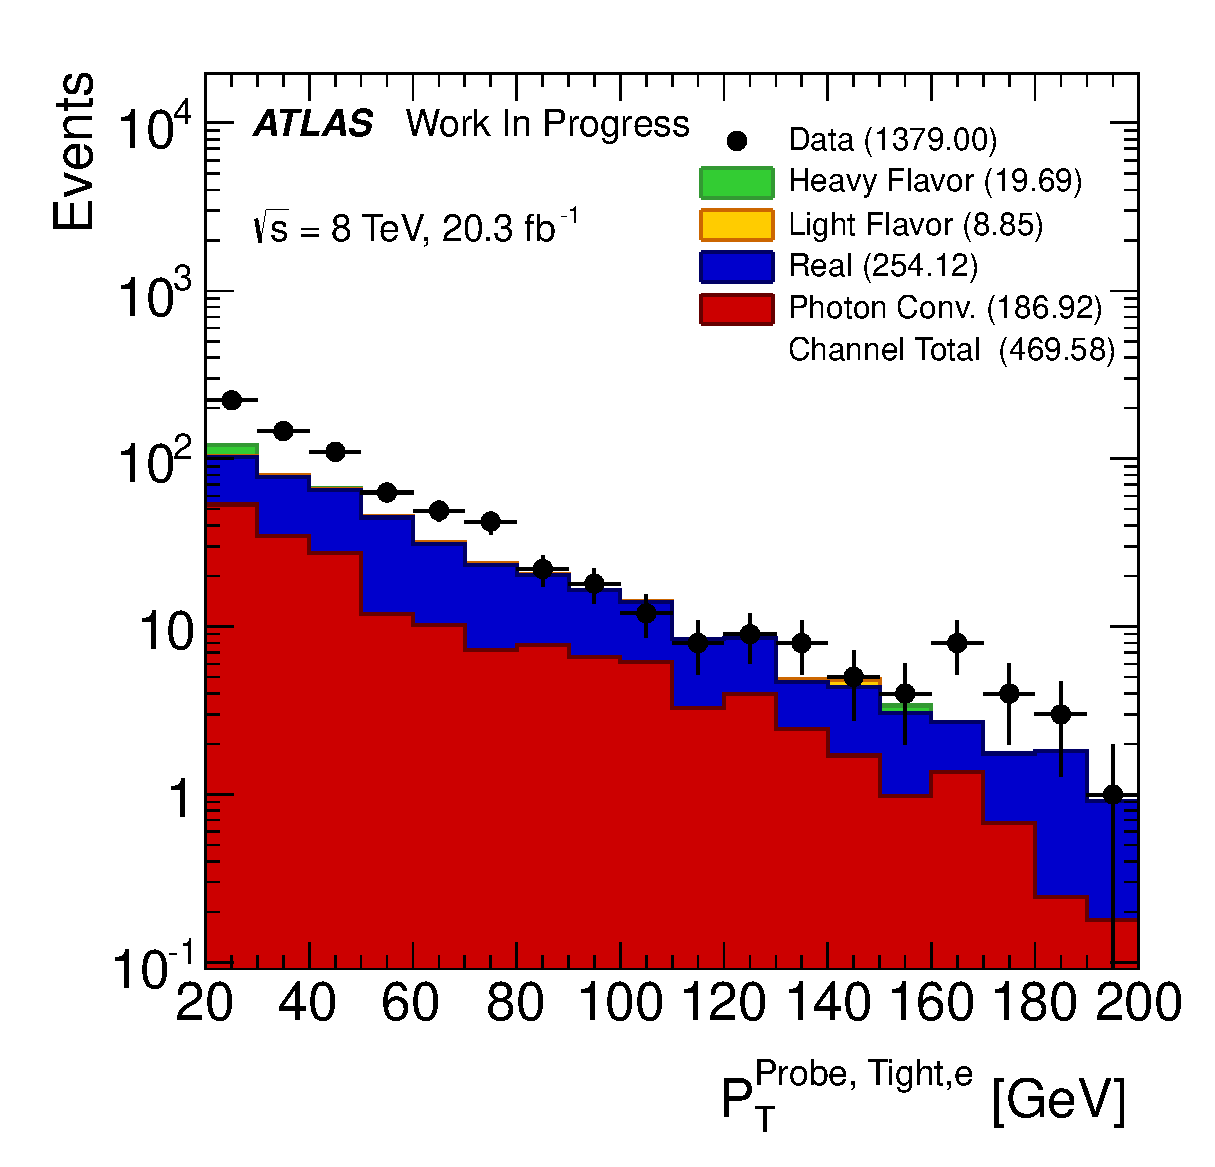
\includegraphics[width=0.45\columnwidth]{figures/fakes_bkg/CRs/SameSignElectronMuon/Stacked/ProbeTightElectronPt.eps}
}
%\centering
%\subfigure{
%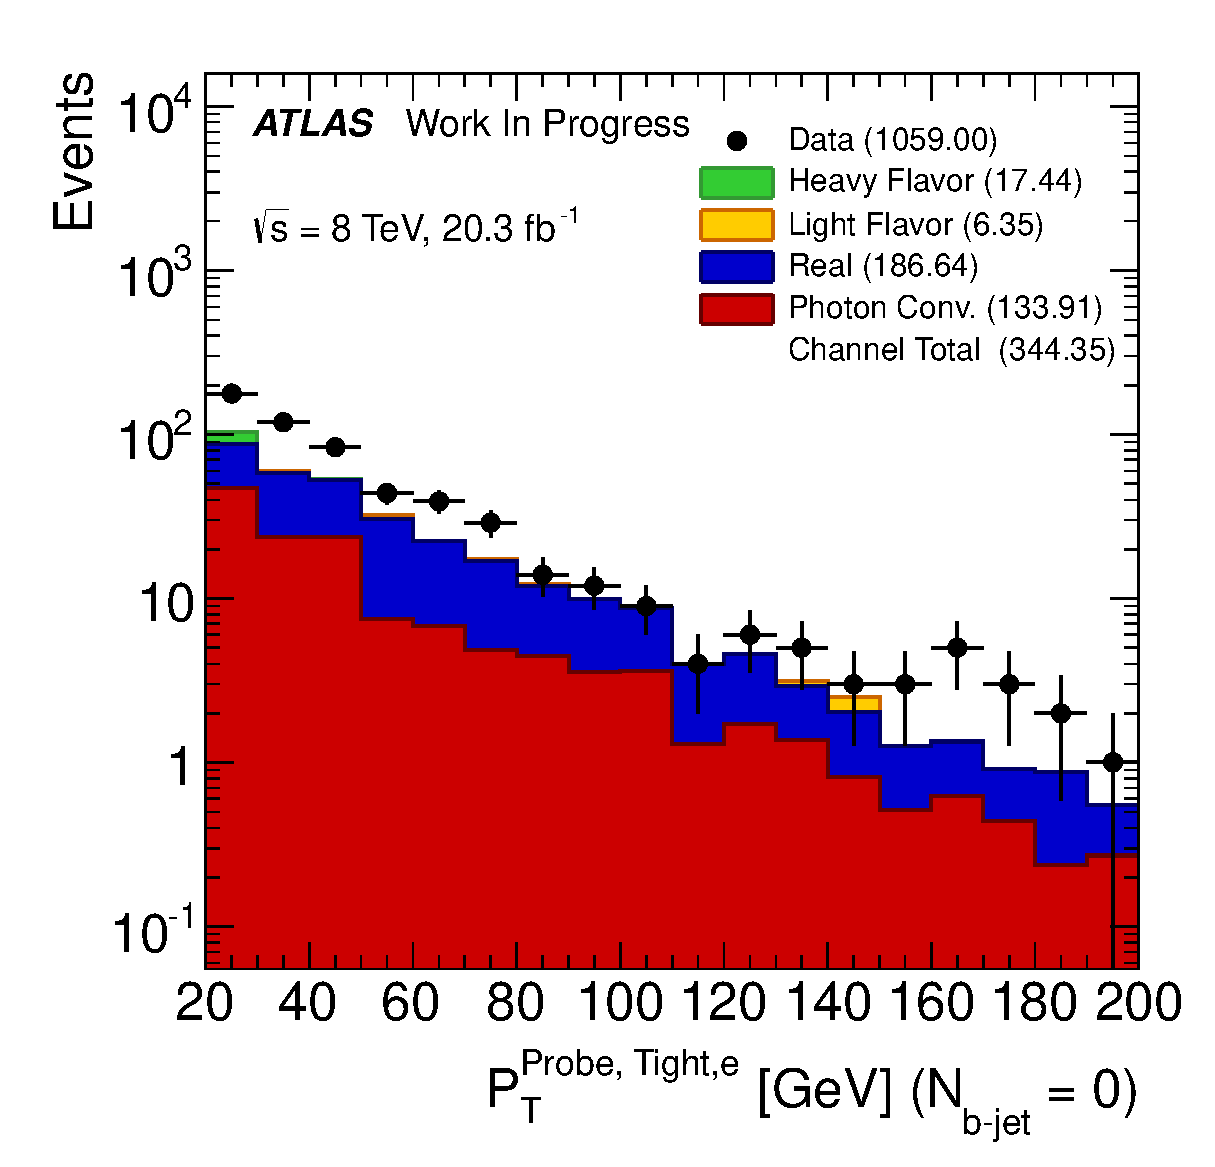
\includegraphics[width=0.3\columnwidth]{figures/fakes_bkg/CRs/SameSignElectronMuon/Stacked/ProbeTightElectronPtBJetEq0.eps}
%}
\centering
\subfigure{
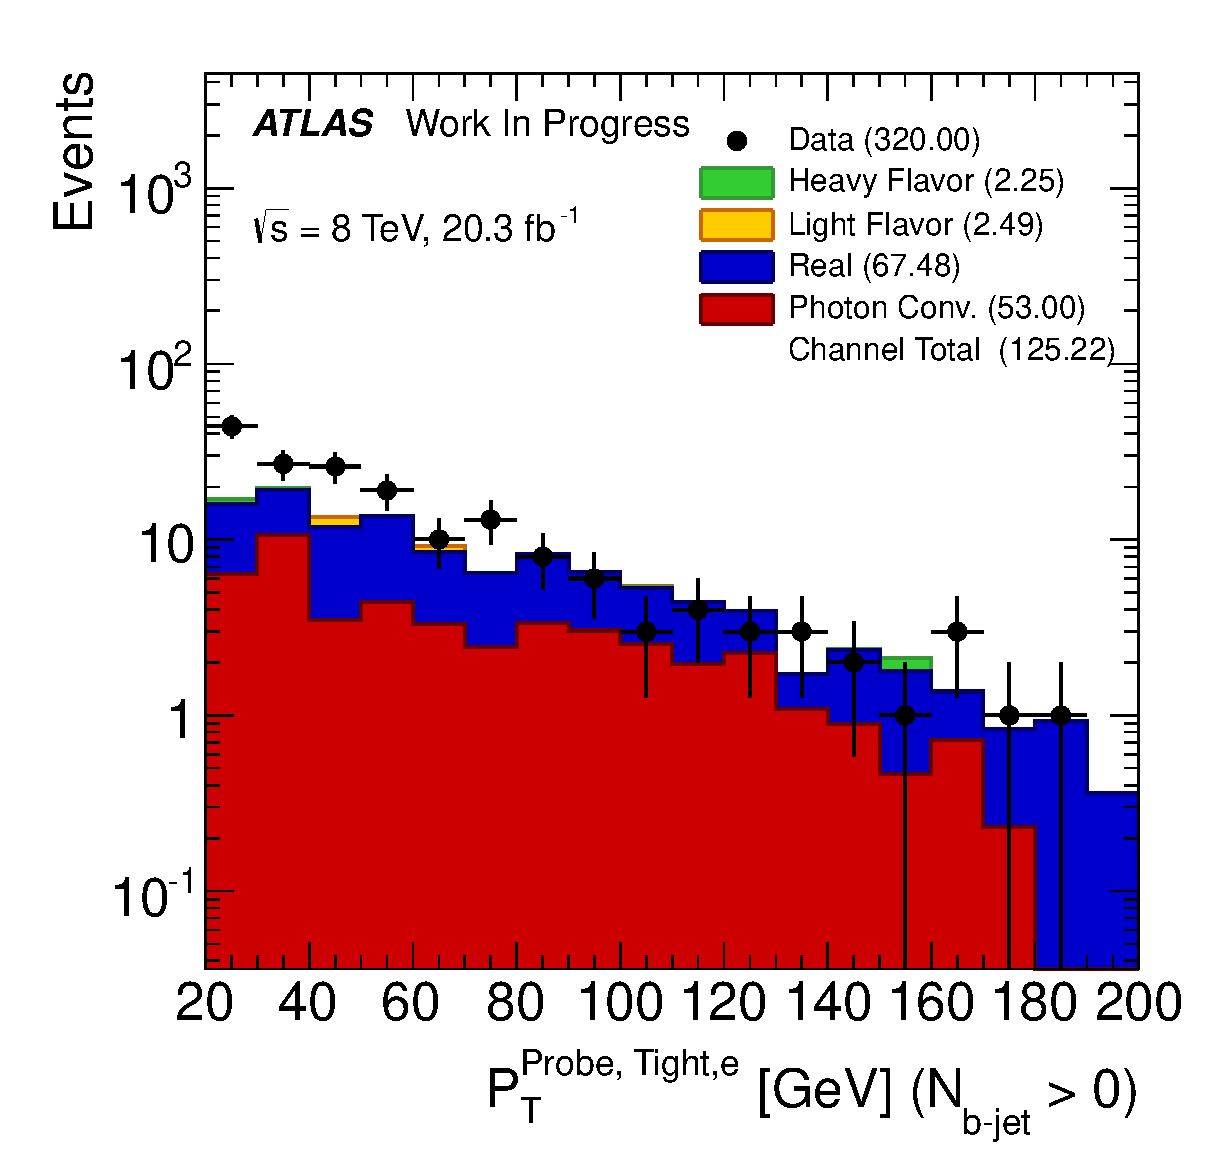
\includegraphics[width=0.45\columnwidth]{figures/fakes_bkg/CRs/SameSignElectronMuon/Stacked/ProbeTightElectronPtBJetGt0.eps}
}
\centering
\subfigure{
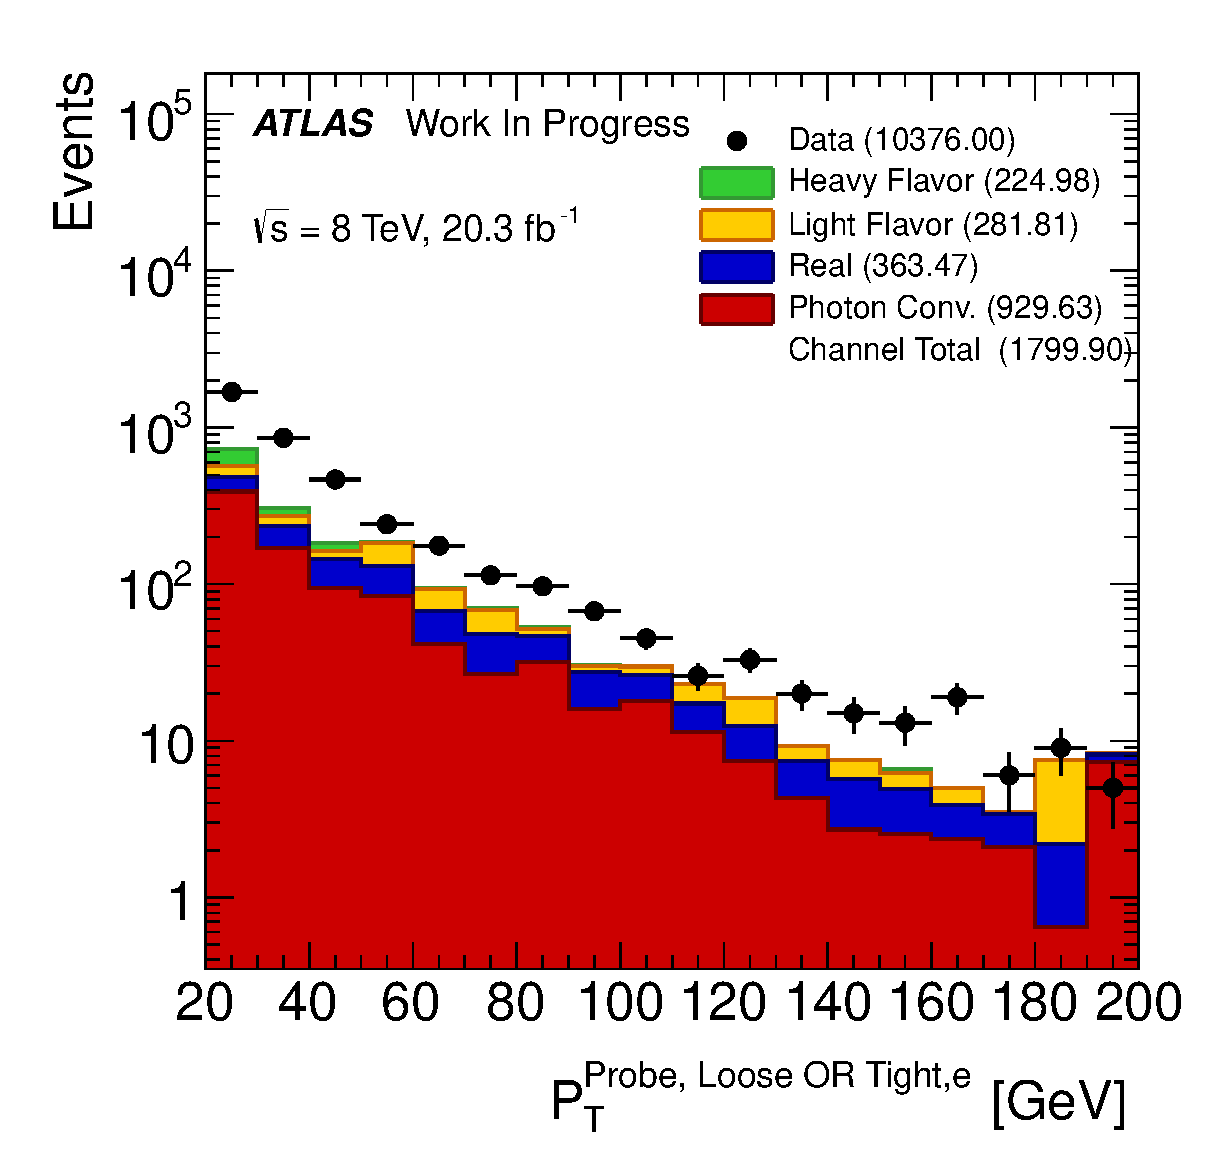
\includegraphics[width=0.45\columnwidth]{figures/fakes_bkg/CRs/SameSignElectronMuon/Stacked/ProbeLooseORTightElectronPt.eps}
}
%\centering
%\subfigure{
%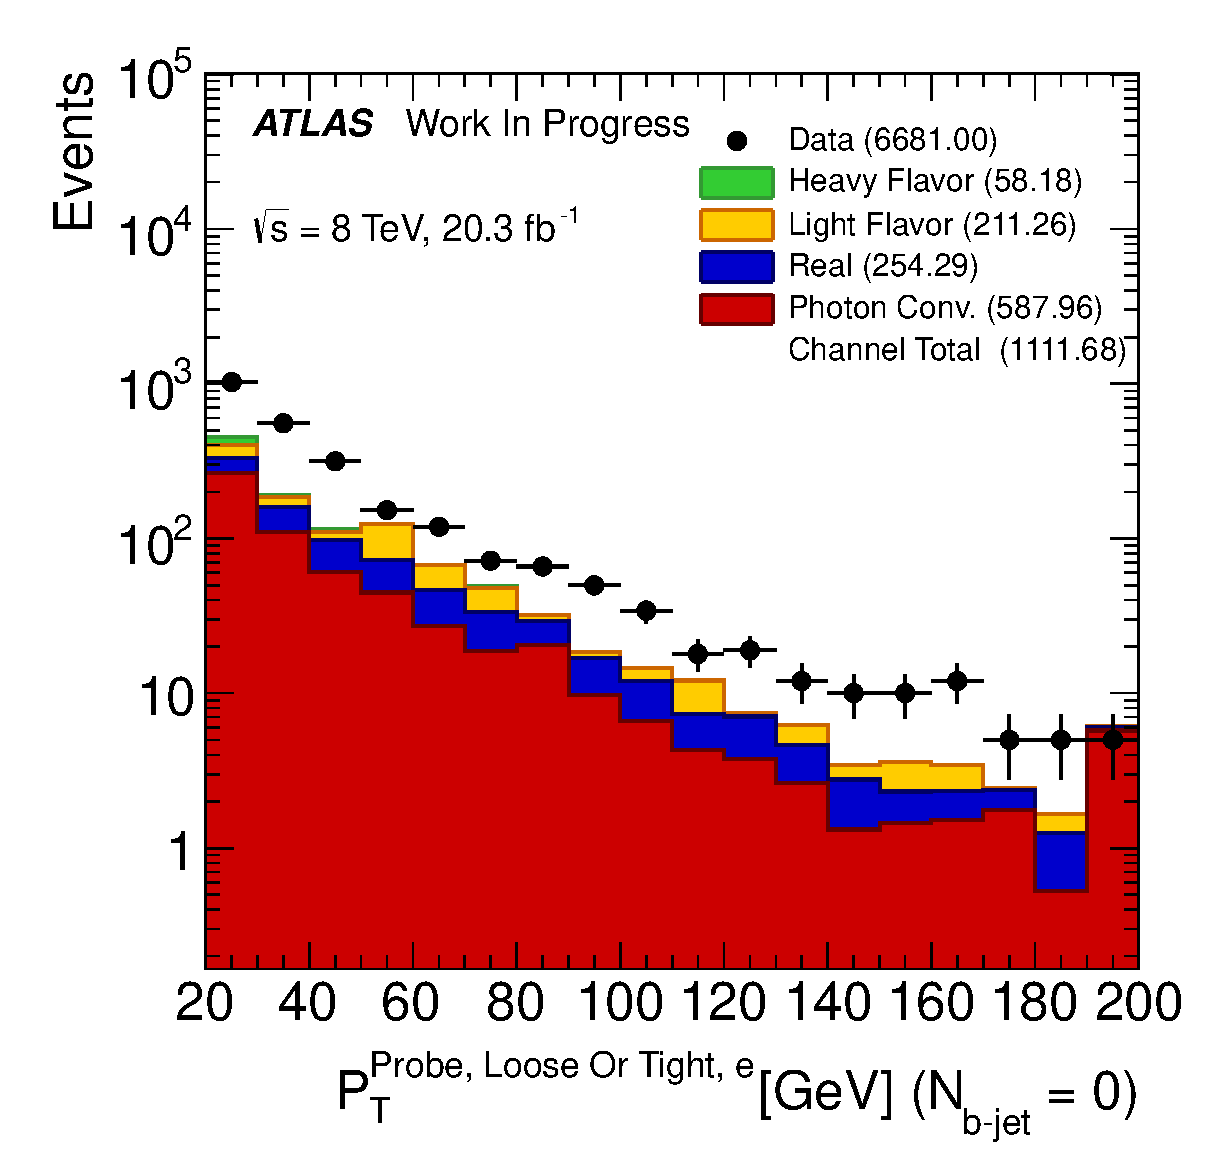
\includegraphics[width=0.3\columnwidth]{figures/fakes_bkg/CRs/SameSignElectronMuon/Stacked/ProbeLooseORTightElectronPtBJetEq0.eps}
%}
\centering
\subfigure{
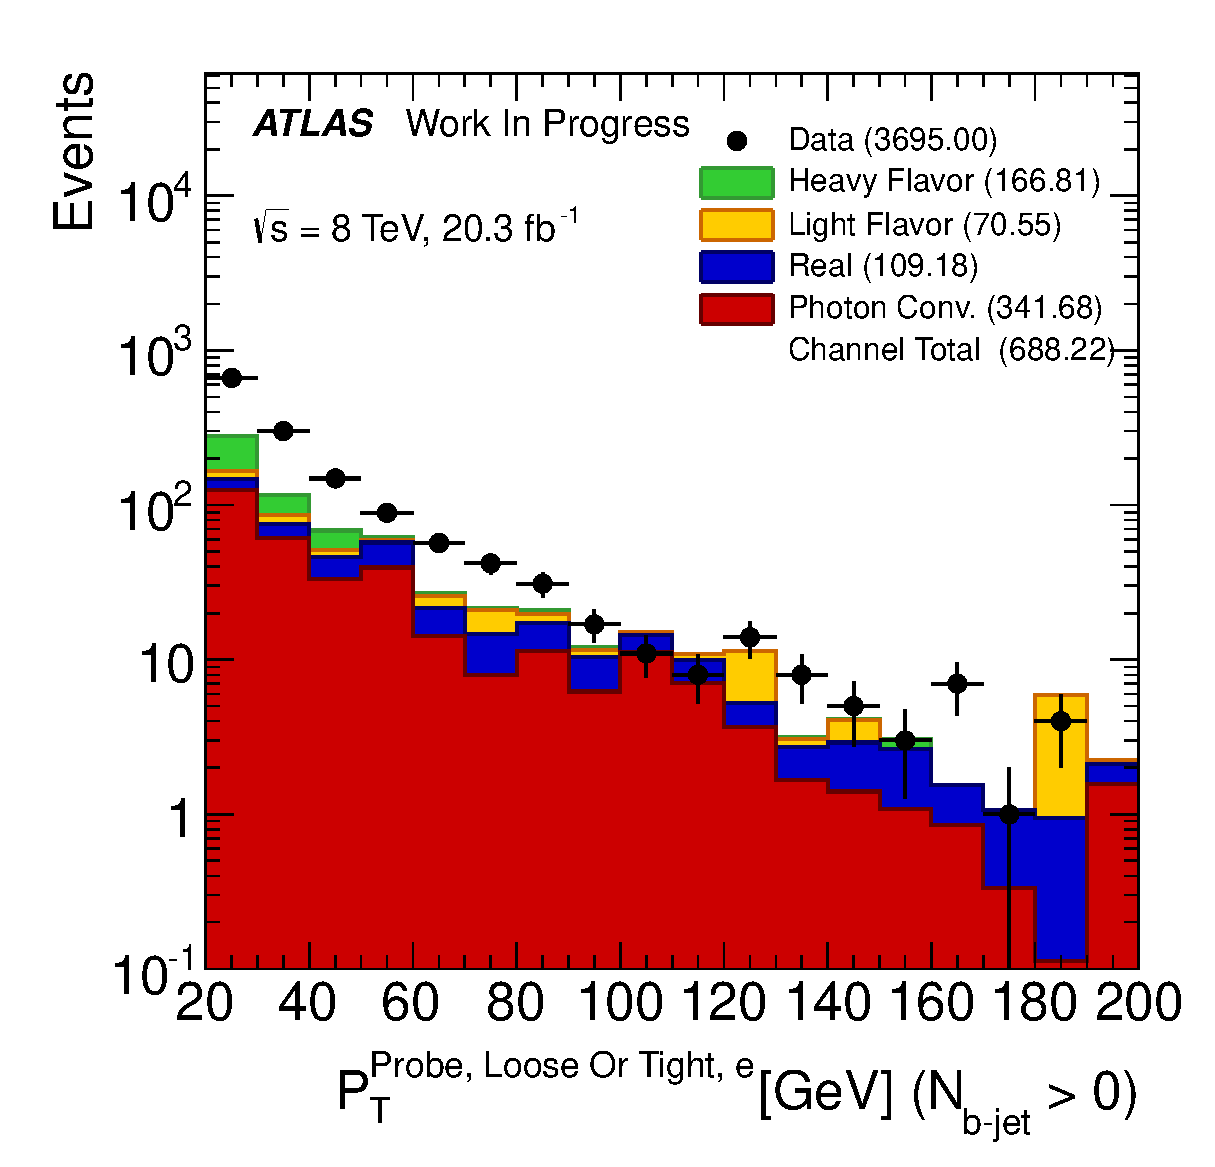
\includegraphics[width=0.45\columnwidth]{figures/fakes_bkg/CRs/SameSignElectronMuon/Stacked/ProbeLooseORTightElectronPtBJetGt0.eps}
}
%\vspace{-1mm}
\vspace{-10mm}\caption{Transverse momentum distributions \pt\ of tight probe electron (top) and loose or tight probe electrons (bottom) passing signal selection criteria in the Same-Sign $e-\mu$ control region without any additional requirement on $b$-jets in the event (left) and at least one $b$-jet (right).
The amount observed in data (black points) corresponds to $n$ (bottom) and $n_{\textrm{Tight}}$ (top) in Eq.~\ref{eq:fakerate}. 
Meanwhile, the contribution determined in MC to come from real leptons (blue), photon conversion (red), heavy flavor (green) and light
flavor (orange) are shown stacked on top of each other.
The difference between the data and MC does not effect the data-driven
fake estimate but may have an impact on the composition estimate.
}
\label{fig:fakeEff_CRs_electron_stacked}
\end{figure}

%%%%%%%%%%%scaled

%\begin{figure}[h!]
%\centering
%\subfigure{
%\includegraphics[width=0.45\columnwidth]{figures/fakes_bkg/CRs/SameSignMuonMuon/Scaled/coarse/ProbeTightMuonPtFakeRate_histratio.png}
%}
%\centering
%\subfigure{
%\includegraphics[width=0.45\columnwidth]{figures/fakes_bkg/CRs/SameSignMuonMuon/Scaled/coarse/ProbeTightMuonPtBJetGt0FakeRate_histratio.png}
%}
%\centering
%\subfigure{
%\includegraphics[width=0.45\columnwidth]{figures/fakes_bkg/CRs/SameSignMuonMuon/Scaled/coarse/ProbeLooseORTightMuonPtFakeRate_histratio.png}
%}
%\centering
%\subfigure{
%\includegraphics[width=0.45\columnwidth]{figures/fakes_bkg/CRs/SameSignMuonMuon/Scaled/coarse/ProbeLooseORTightMuonPtBJetGt0FakeRate_histratio.png}
%}
%\vspace{-10mm}\caption{Scaled....Transverse momentum distributions \pt\ of tight probe muons (top) and loose OR tight probe muons (bottom) passing signal selection criteria in the control Same-Sign $\mu-\mu$ control region without any additional requirement on $b$-jets in the event (left) and at least one $b$-jet (right). 
%The amount observed in data (black points) corresponds to $n$ (bottom) and $n_{\textrm{Tight}}$ (top) in Eq.~\ref{eq:fakerate}. 
%Meanwhile, the contribution determined in MC to come from real leptons (blue), photon conversion (red), heavy flavor (green) and light
%flavor (orange) are shown stacked on top of each other. 
%The difference between the data and MC does not effect the data-driven
%fake estimate but may have an impact on the composition estimate.
%}
%\label{fig:fakeEff_CRs_muon_stacked_scaled}
%\end{figure}

%\begin{figure}[h!]
%\centering
%\subfigure{
%\includegraphics[width=0.45\columnwidth]{figures/fakes_bkg/CRs/SameSignElectronMuon/Scaled/coarse/ProbeTightElectronPtFakeRate_histratio.png}
%}
%\centering
%\subfigure{
%\includegraphics[width=0.45\columnwidth]{figures/fakes_bkg/CRs/SameSignElectronMuon/Scaled/coarse/ProbeTightElectronPtBJetGt0FakeRate_histratio.png}
%}
%\centering
%\subfigure{
%\includegraphics[width=0.45\columnwidth]{figures/fakes_bkg/CRs/SameSignElectronMuon/Scaled/coarse/ProbeLooseORTightElectronPtFakeRate_histratio.png}
%}
%\centering
%\subfigure{
%\includegraphics[width=0.45\columnwidth]{figures/fakes_bkg/CRs/SameSignElectronMuon/Scaled/coarse/ProbeLooseORTightElectronPtBJetGt0FakeRate_histratio.png}
%}
%\vspace{-10mm}\caption{Scaled...Transverse momentum distributions \pt\ of tight probe electron (top) and loose or tight probe electrons (bottom) passing signal selection criteria in the Same-Sign $e-\mu$ control region without any additional requirement on $b$-jets in the event (left) and at least one $b$-jet (right).
%The amount observed in data (black points) corresponds to $n$ (bottom) and $n_{\textrm{Tight}}$ (top) in Eq.~\ref{eq:fakerate}. 
%Meanwhile, the contribution determined in MC to come from real leptons (blue), photon conversion (red), heavy flavor (green) and light
%flavor (orange) are shown stacked on top of each other.
%The difference between the data and MC does not effect the data-driven
%fake estimate but may have an impact on the composition estimate.
%}
%\label{fig:fakeEff_CRs_electron_stacked_scaled}
%\end{figure}


\begin{table}[ht!]
\centering
\begin{tabular}{|lc|ccc|}
    \hline
    \multicolumn{5}{|c|}{\bf{Control regions}}   \\ \hline \hline
    PC subtracted &$N_{b-jet}$  &{HF} &{PC} &{LF} \\ \hline
    yes &--- &$57\pm 4$\%  &$0$\% &$43\pm 6$\% \\
    yes &$N_{b-jet}>0$  &$75\pm 5$\% &$0$\% &$25\pm 3$\% \\ \hline
    no &--- &$22\pm 3$\% &$61\pm 13$\% &$17\pm 3$\% \\
    no &$N_{b-jet}>0$  &$43\pm 3$\% &$42\pm 6$\% &$15\pm 2$\% \\ 
    \hline
	
\end{tabular}




\caption{
Composition of fake electrons taken from  MC events in the same-sign electron-muon di-lepton control regions
used to extract electron fake rates. The composition is split as either Heavy Flavor (HF), Photon
Conversion (PC), and Light Flavor (LF) are shown. In the ``PC subtracted'' case, the PC component
has been explicitly removed.  This corresponds to the scenario ultimately used in the
fake rate estimation.
}
\label{table:CompositionElectronCR}
\end{table}

\begin{table}[ht!]
\centering
    \begin{tabular}{|l||cc|}
    \hline 
    \multicolumn{3}{|c|}{\bf{Pre-selection and signal regions}}   \\ 
    & Heavy Flavor & Light Flavor \\
    \hline \hline
    \hline

    Pre-selection &$53.7 \pm 9.4$\% & $46.3\pm 10.0$\% \\
    0 SFOS &$80.2 \pm 19.9$\% & $19.8\pm 11.8$\% \\
    1 SFOS &$52.4 \pm 12.5$\% & $47.6\pm 11.9$\% \\
    2 SFOS &$47.7 \pm 16.1$\% & $52.3\pm 23.3$\% \\
    \hline


  \end{tabular}
  








\caption{
Composition of fake electrons taken from  MC events in the event pre-selection and regions close to the signal regions used in the analysis. 
The composition is split as either Heavy Flavor (HF) or Light Flavor (LF). 
}
\label{table:CompositionElectronSR}
\end{table}


\begin{table}[ht!]
\centering
    \begin{tabular}{|lc|ccc|}
    \hline
    \multicolumn{5}{|c|}{\bf{Control regions}}   \\ \hline \hline
    PC subtracted &$N_{b-jet}$  &{HF} &{PC} &{LF} \\ \hline
    yes &--- &$89\pm 4$\% &$0$\% &$11\pm 1$\% \\
    yes &$N_{b-jet}>0$  &$95\pm 3$\% &$0$\% &$4\pm 1$\%\\ \hline
    no &--- &$89\pm 4$\% &$0$\% &$11\pm 1$\% \\
    no &$N_{b-jet}>0$  &$95\pm 3$\% &$0$\% &$4\pm 1$\%\\ 
    %\color{yellow!70!black}\met\ $>10$GeV &\color{yellow!70!black}$N_{b-jet}>1$  &\color{yellow!70!black}91\% &\color{yellow!70!black}0\% &\color{yellow!70!black}9\% \\ 
    \hline
  \end{tabular}
  

\caption{
Composition of fake muons taken from  MC events in the event pre-selection and regions close to the signal regions used in the analysis. 
The composition is split as either Heavy Flavor (HF), Photon
Conversion (PC), and Light Flavor (LF) are shown. The photon conversion component
is measured to be negligible. No PC subtraction is performed.
}
\label{table:CompositionMuonCR}
\end{table}

\begin{table}[ht!]
\centering
    \begin{tabular}{|l||cc|}
    \hline 
    \multicolumn{3}{|c|}{\bf{Pre-selection and signal regions}}   \\ 
    & Heavy Flavor & Light Flavor \\
    \hline \hline
    \hline

    Pre-selection &$78.9 \pm 10.0$\% & $21.1\pm 4.6$\% \\
    0 SFOS &$96.7 \pm 21.0$\% & $3.3\pm 3.7$\% \\
    1 SFOS &$77.4 \pm 14.1$\% & $22.6\pm 7.2$\% \\
    2 SFOS &$77.3 \pm 15.9$\% & $22.8\pm 7.1$\% \\
    \hline


  \end{tabular}
  








\caption{
Composition of fake muons taken from  MC events in the same-sign muon-muon di-lepton control regions
used to extract the muon fake rates. The composition is split into either Heavy Flavor (HF) or Light Flavor (LF). 
}
\label{table:CompositionMuonSR}
\end{table}

\clearpage
\subsubsection{Fake lepton background validation}

A Monte Carlo closure test of the generalized matrix method is performed. The fake rates are computed from MC samples in the di-lepton control regions defined in section~\ref{sec:fakecomposition}, and the method is then applied on the most important MC samples contributing to the event pre-selection: $Z$+jets and $t\bar{t}$. The event pre-selection is used for this test, because the statistics available for the MC samples containing fake leptons in the signal region is too small to be able to draw any conclusion. Figure~\ref{fig:MCFakeRatesClosure}, show the MC fake rates obtained from the CR, while figure~\ref{fig:MCClosureCheckMatrixMethod} show the MC agreement with the MC events re-weighted using the generalized matrix method in the event pre-selection region, for the third-leading lepton $\pt$ and the $\met$ distribution. As it can be seen the shape agreement and the overall normalization are pretty good, showing that the matrix method is performing well.

\begin{figure}[ht!]
\centering
\includegraphics[width=0.42\columnwidth]{figures/ClosureCheck_MatrixMethod/ElFakeRates_MC_topZjets_new.pdf}
\includegraphics[width=0.42\columnwidth]{figures/ClosureCheck_MatrixMethod/MuFakeRates_MC_topZjets_new.pdf}
\caption{Distribution of the fake rates obtained from MC samples in the di-lepton control regions. The errors shown here are statistical only. These rates are used to performed a MC closure check of the global matrix method.}
\label{fig:MCFakeRatesClosure}
\end{figure}

\begin{figure}[ht!]
\centering
\includegraphics[width=0.42\columnwidth]{figures/ClosureCheck_MatrixMethod/PtThirdLepSignal_TTT_total_new.pdf}
\includegraphics[width=0.42\columnwidth]{figures/ClosureCheck_MatrixMethod/VR_PMET_lepTTT_total_new.pdf}
\caption{Distributions of the third leading lepton $\pt$ and $\met$ in the event pre-selection region, for $Z$+jets and $t\bar{t}$, compared to events from these samples re-weighted using the global matrix method and the rates shown in Figure~\ref{fig:MCFakeRatesClosure}. Good agreement is observed}
\label{fig:MCClosureCheckMatrixMethod}
\end{figure}




The ability of the generalized matrix method just described to model accurately
the fake lepton background is tested in a control region designed to be enhanced
in the fake lepton background while maintaining orthogonality with the signal
regions described in Section~\ref{sec:signal_regions}. The control region 
starts by using the event pre-selection region described in Section~\ref{sec:preselection}. To reduce contamination in the 
control region from the $WZ$ process, it is required that none
of the three leptons selected form a Same-Flavor Opposite-Sign lepton pair.
Finally, to ensure orthogonality with the signal regions which require that no
$b$-tagged jets are present in the event, this control region requires
the presence of at least one $b$-tagged jet in the event. 

This control region
is clearly dominated by the data-driven fake lepton background as can
be seen in Fig.~\ref{fig:FakeCR} and in Table~\ref{tab:FakeCR}. 
Furthermore, Table~\ref{tab:FakeCR} shows good agreement between data
and the fake background modeling on the total event yield, which is within 
the statistical uncertainties.  One can even see from
Fig.~\ref{fig:FakeCR} that the shape description does a reasonable job,
although the statistical uncertainty is a bit too large to draw strong conclusions.
One can also see that the systematic uncertainty easily covers most
of the differences that are observed. Thus, we conclude that the fake background
description is working and may be used in our signal regions.  Especially since
the fake background is most important in the 0 SFOS region (described in more
detail in Section~\ref{sec:signal_regions}) which differs primarily from this
control region only by the $b$-veto requirement.




\begin{figure}[ht!]
\centering
\includegraphics[width=0.3\columnwidth]{figures/Fake_CR/LeadingLeptonPt_histratio.eps}
\includegraphics[width=0.3\columnwidth]{figures/Fake_CR/SubleadingLeptonPt_histratio.eps}
\includegraphics[width=0.3\columnwidth]{figures/Fake_CR/MinimumLeptonPt_histratio.eps}
\includegraphics[width=0.3\columnwidth]{figures/Fake_CR/MET_Et_histratio.eps}
\includegraphics[width=0.3\columnwidth]{figures/Fake_CR/NBTaggedJets_histratio.eps}
\includegraphics[width=0.3\columnwidth]{figures/Fake_CR/NJets_histratio.eps}
\includegraphics[width=0.3\columnwidth]{figures/Fake_CR/NMuons_histratio.eps}
\caption{Distributions in a control region designed to study the data-driven fake lepton background estimate.  The selection used is as follows: Event pre-selection + 0 SFOS + at least 1 $b$-jet.  Good agreement is observed}
\label{fig:FakeCR}
\end{figure}

\begin{table}[ht!]
\centering
\begin{tabular}{|c||c|c|c|c|}
\hline
 & Event Yield\\ 
\hline\hline
$WZ$ &  $0.338 \pm 0.021$\\ 
$ZZ$ &  $0.0747 \pm 0.0064$\\ 
$Z\gamma$ &  $0.0058 \pm 0.0058$\\ 
$ZWW+ZZZ$ &  $0.026 \pm 0.005$\\ 
$t\bar{t}+V$ &  $3.228 \pm 0.039$\\ 
Fake (data-driven) &  $10.91 \pm 0.73$\\ 
$WWW$ &  $0.1431 \pm 0.0052$\\ 
\hline
Expected Background &  $14.58 \pm 0.73$\\ 
Expected Signal + Background &  $14.72 \pm 0.73$\\ 
\hline
Observed Data &  $18.0 \pm 4.2$\\ 
\hline
\end{tabular}

\caption{Expected and observed yields for the fake lepton control region.}
\label{tab:FakeCR}
\end{table}




